\documentclass[12pt,a4paper]{report}

\usepackage{array}
\usepackage{makecell}
\usepackage{fancyhdr}
\usepackage{microtype}
\usepackage{tabto}
\newcolumntype{L}[1]{>{\raggedright\let\newline\\\arraybackslash\hspace{0pt}}m{#1}}
\newcolumntype{C}[1]{>{\centering\let\newline\\\arraybackslash\hspace{0pt}}m{#1}}
\newcolumntype{R}[1]{>{\raggedleft\let\newline\\\arraybackslash\hspace{0pt}}m{#1}}

\usepackage{mathptmx}
\usepackage{graphicx} % Required for inserting images
\graphicspath{{img/}}
\usepackage{multirow}
\usepackage{caption}
\usepackage{longtable}

\usepackage{geometry}
\geometry{
	top=4cm,
	right=3cm,
	left=4cm,
	bottom=3cm,	
}

\usepackage{pdflscape}
\usepackage{everypage}
\usepackage{tabularray}
\usepackage{listings}
\lstset{
    basicstyle=\fontsize{10}{12}\selectfont\ttfamily,
    linewidth=\dimexpr\linewidth-2cm\relax,
    breaklines=true, % Margin bingkai kanan % Atur ukuran font dan jenis huruf
}
\usepackage[table]{xcolor}
\usepackage{setspace}
\doublespacing


\renewcommand{\thechapter}{\centering \Roman{chapter}}
\renewcommand{\thesection}{\arabic{chapter}.\arabic{section}}

\def\contentsname{DAFTAR ISI}
\renewcommand\bibname{DAFTAR PUSTAKA}
\def\chaptername{BAB}
\usepackage{amsmath}
\usepackage{booktabs}
\usepackage{titlesec}
\titleformat{\chapter}[display]{\normalfont\bfseries\centering}{\MakeUppercase{\chaptertitlename}~\thechapter}{0pt}{}
\titlespacing*{\chapter}{0pt}{-2pt}{16pt}

\renewcommand{\arraystretch}{1.5}

\renewcommand\thechapter{\Roman{chapter}}
\newcommand{\arabicchapter}{\arabic{chapter}}
\renewcommand\thesection{\arabic{section}}
\def\thesection{\arabic{chapter}.\arabic{section}}
\def\thetable{\arabic{table}}


\titleformat{\section}[block]{\bf\normalsize}{\thesection}{0.6em}{}
\titlespacing*{\section}{0pt}{5pt}{0pt}
\titleformat{\subsection}[block]{\bf\normalsize}{\thesubsection}{0.6em}{}
\titlespacing*{\subsection}{0pt}{5pt}{0pt}

\usepackage{setspace}
%\singlespacing
\doublespacing
%\doublespacing
%\setstretch{1.1}
\renewcommand{\tablename}{Tabel}
\renewcommand{\figurename}{Gambar}
\renewcommand{\thefigure}{\arabicchapter.\arabic{figure}}
\renewcommand{\thetable}{\arabicchapter.\arabic{table}}
\usepackage[breaklinks]{hyperref}
\renewcommand{\listfigurename}{DAFTAR GAMBAR}
\renewcommand{\listtablename}{DAFTAR TABEL}

\hyphenation{me-la-in-kan}

\newcommand{\nim}{1990343064}							% NIM Mahasiswa 
\newcommand{\mahasiswa}{Ahlul Mukhramin}	% Nama Mahasiswa
\newcommand{\judulId}{Rancang Bangun Game Online FPS (Jak Meuprang) 3D Menggunakan Photon Unity Networking }
\newcommand{\judulEn}{Thesis Title}
\newcommand{\jurusan}{Jurusan Teknologi Informasi dan Komputer}
\newcommand{\prodi}{Teknologi Rekayasa Komputer Jaringan}
\newcommand{\institusi}{Politeknik Negeri Lhokseumawe}
\newcommand{\pembimbingUtama}{Atthariq, S.ST, MT}
\newcommand{\nipPembimbingUtama}{19780724 200112 1 001}
\newcommand{\pembimbingPendamping}{Hari Toha Hidayat, S.Si., M.Cs}
\newcommand{\nipPembimbingPendamping}{19851014 201404 1 001}
\newcommand{\kajur}{Muhammad Arhami, S.Si., M,Kom}
\newcommand{\nipKajur}{19741029 200003 2 001}
\newcommand{\kaprodi}{Fachri Yanuar Rudi F, SST, MT}
\newcommand{\nipKaprodi}{19880106 201803 1 001}
\newcommand{\ketua}{Aswandi, S.Kom., M.Kom.}
\newcommand{\nipKetua}{19720924 201012 1 001}
\newcommand{\sekretaris}{Afla Nevrisa, S.Kom., M.Kom.}
\newcommand{\nipSekretaris}{19921117 202203 2 007}
\newcommand{\pembahaskedua}{Mursyidah, M.T.}
\newcommand{\nipPembahaskedua}{19730105 199903 2 003}
\newcommand{\resetkem}{KEMENTERIAN PENDIDIKAN, KEBUDAYAAN, RISET, DAN TEKNOLOGI}



\begin{document}
\singlespacing
\begin{center}
    \thispagestyle{empty}
\vfill
\normalsize
\MakeUppercase{\textbf{\judulId}}
    
\vfill
\normalsize
\MakeUppercase{\textbf{skripsi}}

\vfill
\normalsize
Diajukan sebagai salah satu syarat untuk menyelesaikan \\
Pendidikan Jenjang Sarjana Terapan\\
Pada Politeknik Negeri Lhokseumawe.

\vfill
\begin{figure}[h]
\centering
\includegraphics[width=4cm]{logo-pnl}
\end{figure}

\vfill
Oleh: \\
\MakeUppercase{\textbf{\mahasiswa}} \\~\\
\begin{tabular}{ll}
    NIM & : \nim \\
    Program Studi & : \prodi \\
    Jurusan & : \jurusan
\end{tabular}

\vfill
\MakeUppercase{
\textbf{
\resetkem \\
\institusi \\
\the\year{}
}}

\end{center}
\clearpage
\pagenumbering{roman}
\onehalfspacing
\chapter*{PENGESAHAN PEMBIMBING}
\addcontentsline{toc}{chapter}{PENGESAHAN PEMBIMBING}
Skripsi yang berjudul "\judulId", disusun oleh \mahasiswa, NIM \nim, Program Studi Teknologi Rekayasa Komputer Jaringan, Jurusan Teknologi Informasi dan Komputer Politeknik Negeri Lhokseumawe telah memenuhi syarat untuk dipertanggung jawabkan didepan dewan penguji.


\vspace*{1cm}
\noindent 
\tabto{7.84cm}Buket Rata, 02 Agustus 2023\\
\noindent \begin{minipage}[t]{0.45\linewidth}
\noindent
Pembimbing I
  
\vspace*{2cm}
\textbf{\pembimbingUtama} \\
NIP: \nipPembimbingUtama
\end{minipage}
\hspace{0.1\linewidth}
\begin{minipage}[t]{0.45\linewidth}
  \noindent
  Pembimbing II
  
  \vspace*{2cm}
  \textbf{\pembimbingPendamping} \\
  NIP: \nipPembimbingPendamping
\end{minipage}

\vspace*{1cm}
\noindent 
\tabto{5.8cm}Mengetahui,\\
\\
\noindent \begin{minipage}[t]{0.45\linewidth}
\noindent
Ketua Jurusan\\
Teknologi Informasi dan Komputer
  
\vspace*{2cm}
\textbf{\kajur} \\
NIP: \nipKajur
\end{minipage}
\hspace{0.1\linewidth}
\begin{minipage}[t]{0.60\linewidth}
    \noindent
    Ketua Program Studi\\
    \raggedright Teknologi Rekayasa Komputer Jaringan
    
    \vspace*{2cm}
    \textbf{\kaprodi} \\
    NIP: \nipKaprodi
  \end{minipage}
  
  


\chapter*{PENGESAHAN PENGUJI}
\addcontentsline{toc}{chapter}{PENGESAHAN PENGUJI}
\begin{sloppypar}
\noindent
Skripsi yang berjudul "\judulId", disusun oleh \mahasiswa, NIM \nim, Program Studi Teknologi Rekayasa Komputer Jaringan, Jurusan Teknologi Informasi dan Komputer Politeknik Negeri Lhokseumawe telah memenuhi syarat untuk dipertanggung jawabkan didepan dewan penguji dan dinyatakan lulus pada tanggal.
\end{sloppypar}

\vspace*{1cm}
\noindent 
\tabto{5.8cm}Dewan Penguji,\\
\noindent \begin{minipage}[t]{0.45\linewidth}
\noindent
Ketua
  
\vspace*{2cm}
\textbf{\ketua} \\
NIP: \nipKetua
\end{minipage}
\hspace{0.1\linewidth}
\begin{minipage}[t]{0.45\linewidth}
  \noindent
  Sekretaris
  
  \vspace*{2cm}
  \textbf{\sekretaris} \\
  NIP: \nipSekretaris
\end{minipage}

\vspace*{1cm}
\noindent \begin{minipage}[t]{0.43\linewidth}
\noindent
Penguji I,
  
\vspace*{2cm}
\raggedright \textbf{\kaprodi} \\
NIP: \nipKaprodi
\end{minipage}
\begin{minipage}[t]{0.345\linewidth}
  \noindent
  Penguji II,
  
  \vspace*{2cm}
  \textbf{\pembahaskedua} \\
  NIP: \nipPembahaskedua
\end{minipage}
\hspace{0.01\linewidth}
\begin{minipage}[t]{0.35\linewidth}
  \noindent
  Penguji III,
  
  \vspace*{2cm}
  \textbf{\ketua} \\
  NIP: \nipKetua
\end{minipage}


\vspace*{1cm}
\noindent 
\tabto{5.8cm}Mengetahui,\\
\\
\noindent \begin{minipage}[t]{0.45\linewidth}
\noindent
Ketua Jurusan\\
Teknologi Informasi dan Komputer
  
\vspace*{2cm}
\textbf{\kajur} \\
NIP: \nipKajur
\end{minipage}
\hspace{0.1\linewidth}
\begin{minipage}[t]{0.60\linewidth}
    \noindent
    Ketua Program Studi\\
    \raggedright Teknologi Rekayasa Komputer Jaringan
    
    \vspace*{2cm}
    \textbf{\kaprodi} \\
    NIP: \nipKaprodi
  \end{minipage}
  
  


\doublespacing
\tableofcontents
\addcontentsline{toc}{chapter}{DAFTAR ISI}

\singlespacing
\listoftables
\addcontentsline{toc}{chapter}{\listtablename}

\listoffigures
\addcontentsline{toc}{chapter}{\listfigurename}


\singlespacing
\chapter*{ABSTRAK}
\addcontentsline{toc}{chapter}{ABSTRAK}
\noindent
Perkembangan teknologi game pada software dan hardware, khususnya di android, terus
berkembang pesat setiap tahunnya. Kini, aplikasi game dalam skala 3D dapat
dijalankan dengan lancar pada android, dan integrasi antara software dan hardware semakin sem-
purna. Kinerja optimal menciptakan pengalaman bermain yang bervariasi bagi peng-
guna. Dalam peningkatan pengalaman bermain game, bermain secara bersamaan
dengan pemain lain menjadi salah satu cara untuk meningkatkan keseruan. skripsi ini merancang sebuah game bergenre FPS dengan gameplay interaktif yang memungkinkan para pemain mengendalikan karakter yang beraksi dalam dunia game. Selain itu, implementasi synchronous multiplayer memungkinkan pemain bermain secara bersamaan dalam waktu nyata, menciptakan pengalaman yang lebih mendalam dan menyenangkan.
Hasil dari pengujian rancangan game ”Jak Meuprang” menunjukkan bahwa para
pemain berhasil bermain bersama secara realtime, dari pengujian performa dan gui pada masing-masing device sesuai dengan yang dirancang. Pengujian jaringan menggunakan
teknologi Photon juga menunjukkan koneksi yang stabil pada delay, memastikan pengalaman
bermain dalam mode multiplayer dapat dinikmati tanpa hambatan.
\newline
\noindent \textbf{Kata Kunci}: FPS \textit{Multiplayer}, Online \textit{Multiplayer}, \textit{Photon Unity Networking}.
\chapter*{ABSTRACT}
\addcontentsline{toc}{chapter}{ABSTRACT}
\noindent
The development of game technology in software and hardware, especially in PCs, continues
growing rapidly every year. Now, game applications in 3D scale can
run smoothly, and the integration between software and hardware is getting better
full. Optimal performance creates a varied gaming experience for users
To use. In enhancing the gaming experience, play simultaneously
with other players is one way to increase the excitement. This thesis designs an FPS genre game with interactive gameplay that allows players to control characters that act in the game world. In addition, the implementation of synchronous multiplayer allows players to play simultaneously in real time, creating a more immersive and enjoyable experience.
The test results for the game design "Jak Meuprang" show that para
players managed to play together in realtime, and the blackbox test did not
indication of a problem on the game interface. Network testing using
Photon technology also shows a stable connection on delay, ensuring the best experience
playing in multiplayer mode can be enjoyed without a hitch.
\newline
\noindent \textbf{Keywords}: FPS \textit{Multiplayer}, Online \textit{Multiplayer}, \textit{Photon Unity Networking}.
\clearpage
\doublespacing
\pagestyle{myheadings}
\makeatletter
\renewcommand{\sectionmark}[1]{\markboth{}{\bfseries}}
\pagenumbering{arabic}
% \setcounter{page}{1}
\chapter{PENDAHULUAN}
\section{Latar Belakang Masalah}
\noindent

\textit{Game} atau permainan adalah aktivitas yang dilakukan untuk tujuan hiburan atau kompetisi, dengan aturan yang telah ditentukan dan biasanya memiliki elemen interaktif yang melibatkan satu atau lebih peserta. \textit{Game} sering kali melibatkan strategi, kecepatan, keterampilan, atau ketangkasan fisik, tergantung pada jenisnya. Tujuan dari \textit{game} adalah untuk mencapai kemenangan, skor tinggi, atau hanya untuk kesenangan semata. \textit{Game} bisa dimainkan secara individu atau dalam kelompok, dan dapat berupa permainan fisik seperti sepak bola, permainan papan seperti catur atau permainan video seperti Mario Bros\cite{fps}.

\textit{First Person Shooter} merupakan sebuah permainan peperangan menggunakan senjata api dengan sudut pandang orang pertama dan hanya menampilkan senjata yang digunakan.
Dalam permainan FPS, pemain biasanya melawan musuh secara langsung dalam pertempuran yang cepat dan intens\cite{fps}. Senjata api menjadi alat utama pemain dalam memerangi musuh.
Agar \textit{game} \textit{First Person Shooter} (FPS) lebih menarik dimainkan, peniliti menambahkan fitur \textit{multiplayer} agar dapat dimainkan bersama sama secara online yang dapat terhubung dimana saja dengan menggunakan koneksi internet. Untuk membuat fitur \textit{multiplayer} peniliti menggunakan \textit{game} engine unity dan framework photon unity networking.

Sistem \textit{multiplayer} pada sebuah \textit{\textit{game}} membuat \textit{\textit{game}} tersebut menjadi lebih interaktif dan menarik untuk dimainkan. Dalam sebuah gim jika pemain memilih untuk single player maka pemain tersebut akan berhadapan dengan lawan NPC (Non Playable Character) sedangkan jika \textit{multiplayer} maka pemain tersebut akan berhadapan dengan pemain lain \cite{Sarwodi}.


Penelitian ini mengusulkan sebuah \textit{\textit{game}} dengan memanfaatkan koneksi via internet yang dapat memainkan \textit{\textit{game}} bertema \textit{first person shooter}, dimana pemain bersaing secara real (nyata) dan lebih menantang di mana minimal ada 2 pemain yang akan bertemu dalam satu room.
Berdasarkan penjabaran diatas, maka diusulkan sebuah judul skripsi yang mengimplementasikan koneksi internet menggunakan photon unity asset pada \textit{\textit{game}} \textit{first person shooter} 3D yang dapat dimainkan menggunakan perangkat laptop/pc dengan judul "Rancang Bangun Game Multiplayer Online First Person Shooter(FPS) 3D Menggunakan Photon Unity Networking".
\textit{\textit{game}} ini akan dibuat \textit{multiplayer} menggunakan fitur dari unity \textit{\textit{game}} engine yaitu photon unity networking.

\section{Rumusan Masalah}
\noindent

Berdasarkan latar belakang masalah yang telah diuraikan, maka didapat perumusan masalah sebagai berikut :
\begin{enumerate}
	\item Bagaimana merancang skenario game fps jak meuprang ?
	\item Bagaimana cara kerja fitur sinkronisasi \textit{multiplayer} online secara \textit{realtime} dengan menggunakan Photon Unity Networking dan data apa saja yang perlu disinkronisasi?
	\item Bagaimana mekanisme alur kerja \textit{first person shooter}(fps) \textit{multiplayer} dari proses persiapan bermain, mulai bermain sampai menyelesaikan permainan?
	\item Berapa persen tingkat keberhasilan pengukuran performa jaringan pada saat game dimainkan?
\end{enumerate}

\section{Batasan Masalah}
\noindent

Pada penelitian ini terdapat batasan masalah dengan maksud untuk mempermudah penulis, adapun batasan masalah pada penelitian ini sebagai berikut:
\begin{enumerate}
	\item Pembuatan \textit{\textit{game}} ini akan menggunakan IDE Unity dan bahasa pemrograman C\#.
	\item Total maksimum CCU (\textit{Concurent Users}) yang dapat terhubung ke Photon Cloud yaitu 5 CCU.
	\item Hanya dapat dimainkan diplatform Android.
	\item Hanya dapat dimainkan jika perangkat terhubung dengan koneksi internet.
	\item Tersedia sound.
	\item Tersedia senjata sebanyak 3 jenis yaitu \textit{rifle}, pistol dan pisau.
	\item Menggunakan assets open source.
	\item Tersedia Map.
	\item Terdapat dua karakter berbeda saat dimainkan.
\end{enumerate}

\section{Tujuan Penelitian}
\noindent

Adapun tujuan dari penelitian ini sebagai berikut :
\begin{enumerate}
	\item Untuk menghasilkan skenario game \textit{deathmatch} pada game fps jak meuprang.
	\item Untuk mengetahui apa saja yang disinkronisasikan pada game tersebut.
	\item Untuk mengetahui \textit{gameplay game} jak meuprang.
	\item Untuk mengetahui ke-stabilan kinerja jaringan, latensi, penggunaan bandwidth, dan lainnya. 
\end{enumerate}

% \section{\textit{Rood Map}}
% \noindent

% Penelitian pertama diambil dari jurnal dengan judul "Pengembangan Game Indonesia Untuk Permainan First Person Shooter (FPS) 3D Multiplayer “CODE TO SHOOT” Menggunakan UNITY NETWORK (UNET) Berbasis Mobile".
% Penilitian ini bertujuan untuk merancang game multiplayer bergenre fps yang dapat dimainkan tanpa harus memasukan alamat ip dan game ini hanya dapat dimainkan diandroid dan tidak dapat dimainkan di laptop/pc\cite{fps}.

% Penelitian kedua diambil dari jurnal dengan judul "Penerapan Multiplayer Pada Gim Tower Defense Menggunakan Photon Unity". Penilitian ini bertujuan merancang game multiplayer bergenre strategi, yang bertujuan untuk mempertahankan wilayah atau harta benda pemain. Hasil penilitian ini berhasil menciptakan game bergenre strategi yang dapat dimainkan secara multiplayer dengan menggunakan photon unity\cite{Sarwodi}.

% Penilitian ketiga diambil dari jurnal dengan judul "Pembuatan Multiplayer Game Ucing Beling Menggunakan Asset 
% Store Mirror". Penilitian ini bertujuan merancang game multiplayer tradisional yang berasal dari jawa barat menggunakan \textit{Asset Store Mirror}. Hasil penilitan penulis menciptakan game menggunakan \textit{Asset Store Mirror}\cite{Ansori}.

% Penelitian keempat diambil dari jurnal dengan judul "Pengembangan Game Multiplayer Pengenalan 
% Budaya Gebug Ende Seraya Karangsem Berbasis 
% Android". Penilitian ini bertujuan merancang game sebagai media pengetahuan berbasis budaya yang dapat membantu masyarakat untuk lebih mengenal budaya khususnya Gebug Ende Seraya Karangsem. Hasil penilitian ini berhasil mencipatkan game yang dapat dimainkan secara multiplayer\cite{Gebug}.

% Penilitian kelima diambil dari jurnal dengan judul "Pembangunan \textit{Game} Mulitiplayer Edukasi GO GREEN 3D
% Berbasu Android". Penilitian ini bertujuan untuk merancang game dengan tema kebersihan yang dapat dimainkan secara multiplayer menggunakan Google Play Games Realtime Multiplayer. Dari jurnal ini terdapat perbedaan yaitu penulis menggunakan google play realtime multiplayer\cite{gogreen}.

\section{Manfaat Penelitian}
Manfaat dari penilitian ini antara lain adalah : 
\begin{enumerate}
	\item Memberikan hiburan dan melatih ketangkasan bermain 
	kepada pengguna.
	\item Untuk mengetahui performa jaringan photon cloud yang dimiliki photon unity networking.
	\item Sebagai bentuk implementasi konsep photon unity networking pada \textit{\textit{game}} first person shooter(fps).
\end{enumerate}

\section{Sistematika Penulisan}
\noindent

Dalam penyusunan skripsi ini, penulis memiliki sistematika penulisan agar 
penulisan skripsi ini terarah dan jelas. Adapun sistematika penulisan laporan yang 
penulis buat adalah sebagai berikut:

\vspace*{1cm}
\noindent\begin{minipage}[t]{0.2\linewidth}
	\noindent \textbf{BAB I}
\end{minipage}
\begin{minipage}[t]{0.8\linewidth}
  \noindent
  \textbf{PENDAHULUAN}\\
  Dalam bab ini menjelaskan tentang latar belakang, rumusan 
  masalah, batasan masalah, tujuan penelitian, Rood Map, manfaat 
  penelitian dan sistematika penelitian.
\end{minipage}
\\
\\
\begin{minipage}[t]{0.2\linewidth}
	\noindent \textbf{BAB II}
\end{minipage}
\begin{minipage}[t]{0.8\linewidth}
  \noindent
  \textbf{TINJAUAN PUSTAKA}\\
  Dalam bab ini menjelaskan tentang pengertian game, \textit{First Person Shooter (FPS)}, Multiplayer, Photon Unity Networking Dan \emph{Quality Of Services (QOS).}
\end{minipage}
\\
\\
\begin{minipage}[t]{0.2\linewidth}
	\noindent \textbf{BAB III}
\end{minipage}
\begin{minipage}[t]{0.8\linewidth}
  \noindent
  \textbf{METODE PENELITIAN}\\
  Dalam bab ini menjelaskan tentang rancangan dan proses yang 
  dilakukan penulis, bagian ini berisikan data dan pengumpulan data, 
  analisa, rancangan sistem (software/hardware), rancangan Use Case 
  Diagram, Story Board dan Teknik Pengujian.
\end{minipage}
\\
\\
\begin{minipage}[t]{0.2\linewidth}
	\noindent \textbf{BAB IV}
\end{minipage}
\begin{minipage}[t]{0.8\linewidth}
  \noindent
  \textbf{HASIL DAN PEMBAHASAN}\\
  Dalam bab ini menjelaskan hasil dari penelitian yang dilakukan 
  penulis, bagian ini berisikan tentang hasil, pembahasan, online dan 
  hasil pengujian.
\end{minipage}
\\
\\
\begin{minipage}[t]{0.2\linewidth}
	\noindent \textbf{BAB V}
\end{minipage}
\begin{minipage}[t]{0.8\linewidth}
  \noindent
  \textbf{PENUTUP}\\
  Bab ini akan menguraikan tentang kesimpulan dan saran dari 
penelitian ini.
\end{minipage}



\chapter{TINJAUAN PUSTAKA}

\section{\textit{State of the Art}}
\noindent

\textit{State of the Art} Dalam penyusunan penilitian ini, peniliti mengambil beberapa referensi terdahulu sebagai panduan penulis untuk penilitian yang dilakukan, yang kemudian  akan menjadi acuan dan perbedaan dari penilitian yang akan dilakukan dengan penilitian sebelumnya. Pemaparan \textit{State of the Art} dapat dilihat pada tabel \ref{tab:stateofart} berikut.

Ada lima penelitian terdahulu yang dianggap sebagai state of the art dalam penelitian ini. Penelitian-penelitian ini dijadikan sebagai dasar acuan yang membantu dalam mengidentifikasi persamaan dan perbedaan antara penelitian ini dan penelitian sebelumnya yang terkait. Judul penelitian ini adalah "\judulId"

\begin{landscape}
	\pagestyle{empty}
    \small % Mengurangi ukuran teks menjadi kecil
    \singlespacing
    \begin{longtable}{|p{1cm}|p{3cm}|p{4cm}|p{2cm}|p{5cm}|p{2.5cm}|p{2.5cm}|}
        \caption{State of the Art}
        \label{tab:stateofart}\\
        \hline
        No & Penulis/Tahun & Judul Artikel & Metode yang digunakan & Hasil yang diperoleh & Persamaan & Perbedaan \\ \hline
        \endfirsthead
        %
        \endhead
        %
        1 & Ibnu Ramadhan, Agung Purwanto, dan Nurahman (2020) & Pengembangan Teknologi Game Indonesia Untuk Permainan FPS 3D Multiplayer “CODE TO SHOOT” Menggunakan Unity Network (UNET) Berbasis Mobile & Unity Network & Game ini dapat dimainkan secara multiplayer tanpa perlu memasukan alamat IP karena fitur uNet dapat bekerja dengan baik. Selain itu game ini juga sudah dapat dimainkan menggunakan platform mobile (Android) & Pembuatan Game Bergenre FPS & Perbedaan Jaringan yang digunakan \\ \hline
        2 & Shena Star Sarwodi, Wibisono Sukmo Wardhono, Muhammad Aminul Akbar (2020) & Penerapan Multiplayer Pada Gim Tower Defense Menggunakan Photon Unity & Photon Unity Networking & Dengan menerapkan Photon Unity Networking pada gim tower defense maka dapat diimplem entasikan sebuah fitur yang dapat meningkatk an interaktivitas dan ketertarikan pemain pada gim yaitu fitur multiplayer. & Menggunakan Photon Unity Networking & Perbedaan diterapkan pada game yang berbeda \\ \hline
        3 & Ryan Nanda Pratama, Anton Siswo Raharjo Ansori, Ashri Dinimaharawati (2021) & Pembuatan Multiplayer Game Ucing Beling Menggunakan Asset Store Mirror & Asset Mirror & Pada multiplayer game Ucing Beling dapat dimainkan secara realtime dan berjalan dengan sesuai yang diharapkan. & Dimainkan secara realtime dan multiplayer & Peneliti menggunakan asset mirror \\ \hline
		4 & I Kadek Budi Suartama, I Gede Mahendra Darmawiguna, dan I Made Putrama (2020) & Pengembangan Game Multiplayer Pengenalan Budaya Gebug Ende Seraya Karangasem Berbasis Android & Metode pengembangan dalam penelitian ini menggunakan GDLC (Game Development Life Cycle) & pengujian blackbox mendapatkan hasil bahwa semua fungsi dan fitur-fitur yang ada dapat berjalan dengan baik dan sebagaimana mestinya. & Persamaannya yaitu menggunakan game engine unity & Perbedaannya terdapat pada metode yang digunakan. \\ \hline
		5 & Muhammad Faisal Fathurrohman Dan Iskandar Ikbal (2018) & PEMBANGUNAN GAME MULTIPLAYER EDUKASI GO GREEN 3D BERBASIS ANDROID & Google Play Games Realtime Multiplayer & Dapat terhubung secara multiplayer menggunakan google play games realtime multiplayer & ersamaannya yaitu sama sama base multiplayer & Perbedaannya terdapat pada google play games realtime multiplayer. \\ \hline
	\end{longtable}
\end{landscape}

\doublespacing
\begin{sloppypar}
\subsection{Penelitian Terdahulu Pertama}
\noindent

Penelitian terdahulu pertama diambil dari jurnal dengan judul "Pengembangan Teknologi Game Indonesia Untuk Permainan FPS 3D Multiplayeer "Code To Shoot" Menggunakan Unity Network (UNET) Berbasis Mobile". Penelitian ini bertujuan untuk membuat game FPS Dengan membawakan tema lokal dari daerah Kalimantan Tengah. Pada pengujian ini peneliti melakukan bermain secara online yang dimana dengan fiture dari UNET sendiri bisa langsung dimainkan tanpa harus memasukan alamat IP.

Perbedaan penelitian ini dengan penelitian yang akan dilakukan terdapat pada penggunaaan \textit{framework}-nya, Penelitian ini menggunakan UNET (Unity Network) sedangkan penelitian yang akan dilakukan menggunakan PUN (Photon Unity Networking).

Persamaan penelitian ini dengan penelitian yang akan dilakukan adalah sama sama \textit{game} bergenre FPS dan \textit{platform} Android.

\subsection{Penelitian Terdahulu Kedua}
\noindent

Penelitian terdahulu kedua diambil dari jurnal dengan judul  "Penerapan Multiplayer Pada Gim Tower Defense Menggunakan Photon Unity". Pada penelitian ini pengujian yang dilakukan yaitu \textit{Exprience Questioner (QEQ)} untuk mengetahui perbedaan pengalaman bermain antara perempuan dan laki-laki, permupan cenderung lebih memiliki perasaan empati dan negatif terhadap lawan bermain, sedangkan pemain jenis laki laki cenderung melibatkan perilaku terhadap lawannya.

Perbedaan penelitian ini dengan penelitian yang akan dilakukan terdapat pada game yang diterapkan, pada penelitian ini game yang diterapkan yaitu game 2D dengan genre Tower Of Defense, sedangkan penelitian yang akan dilakukan yaitu game 3D bergenre FPS.

Persamaan penelitian ini dengan penelitian yang akan dilakukan adalah sama sama menggunakan PUN (Photon Unity Networking).

\subsection{Penelitian Terdahulu Ketiga}
\noindent

Penelitian terdahulu ketiga diambil dari jurnal dengan judul "Pembuatan Multiplayer Game Ucing Beling Menggunakan Asset Store Mirror". Pada penelitian ini pengujian yang dilakukan yaitu dimainkan secara bersama sama apakah permainan dimainkan secara realtime atau secara \textit{server side to side}, dari pengujian yang dilakukan permainan dapat dimainkan secara realtime dan berjalan sesuai dengan yang diharapkan.

Perbedaan penelitian ini dengan penelitian yang akan dilakukan yaitu terhadap framework yang digunakan, pada penelitian ini framework yang digunakan yaitu asset mirror.

Persamaan dari penelitian ini dengan penelitian yang akan dilakukan yaitu sama sama dapat dimainkan secara realtime.

\subsection{Penelitian Terdahulu Keempat}
\noindent

Penelitian terdahulu keempat diambil dari jurnal dengan judul "Pengembangan Game Multiplayer Pengenalan Budaya Gebug Ende Seraya Karangasem Berbasis Android". Pada penelitian ini pengujian yang dilakukan yaitu blackboxnya saja, sebagai pengujian dari penggunaan metode GDLC (\textit{Game Development Life Cycle}) untuk memastikan apakah fitur-fitur yang telah dirancang dapat berjalan dengan semestinya.

Perbedaan penelitian ini dengan penelitian yang akan dilakukan yaitu pada \textit{game} yang dirancang, pada penelitian ini hanya sebatas merancang game sesuai metode GDLC (\textit{Game Development Life Cycle}).

Persamaan dari penelitian ini dengan penelitian yang akan dilakukan yaitu sama sama menggunakan \textit{engine} yang sama yaitu Unity, dan metode yang sama yaitu GDLC(\textit{Game Development Life Cycle}).

\subsection{Penelitian Terdahulu Kelima}
\noindent

Penelitian terdahulu kelima diambil dari jurnal dengan judul "Pembangunan Game Multiplayer Edukasi Go Green 3D Berbasis Android". Pada pengujian yang dilakukan pada penelitian yaitu untuk menguji multiplayer pada game tersebut, pada pengujian yang dilakukan multiplayer berhasil dimainkan secara realtime.

Perbedaan penelitian ini dengan penelitian yang dilakukan yaitu perbeedaan \textit{framework}, pada penelitian ini menggunakan \textit{Google Play Games Realtime Multiplayer}.

Persamaan penelitian ini dengan penelitian yang akan dilakukan sama sama base game multiplayer.
\section{Tinjauan Pustaka}
\subsection{Unity}
\noindent

Unity merupakan salah satu \textit{game} engine paling populer saat ini. Penggunaan Unity dapat digunakan untuk mengembangkan konten interaktif seperti video \textit{game}, 
visualisasi arsitektur, dan real-time 3D animasi. Unity menggunakan bahasa pemograman JavaScript dan 
C\# \parencite{Ansori}. Unity juga merupakan perangkat lunak yang digunakan untuk mengembangkan \textit{game} \textit{multiplatform} yang didesain secara user \textit{friendly} 
(Iman, 2017). Keunggulan Unity adalah Unity 
dapat dengan mudah mengontrol objek-objek 
dalam gim atau aplikasi. Unity terdapat 2 jenis 
lisensi yaitu \textit{personal edition} yang dapat diakses 
secara gratis dan \textit{professional edition} yang 
diharuskan untuk membayar perbulan untuk 
mengaksesnya dengan beberapa fitur tambahan 
yang tidak terdapat di \textit{personal edition} \parencite{Sarwodi}. 

\subsection{\textit{Multiplayer}}
\noindent

\textit{Multiplayer} merupakan fitur pada \textit{game} dimana pemain bermain dengan lebih dari 1 orang yang bermain 
di lingkungan \textit{game} yang sama dan waktu yang bersamaan. \textit{Game} \textit{Multiplayer} biasanya memberikan pilihan pada 
pemain untuk berbagi sumber daya sistem \textit{game} atau menggunakan internet untuk bermain bersama dalam jarak 
jauh. \textit{Game} \textit{Multiplayer} yang terhubung dengan internet melibatkan pemain yang saling terhubung melalui server. 
Sedangkan \textit{Game} \textit{Multiplayer} dengan koneksi lokal yaitu, pemain saling terhubung secara langsung dengan 
pemain lainnya, pemain terkoneksi menggunakan jaringan peer to peer. Pada \textit{Game} \textit{Multiplayer} online memiliki 
beberapa jenis kategori diantaranya adalah \textit{Massively} \textit{Multiplayer} Online \textit{game} (MMO), \textit{Massively} \textit{Multiplayer} 
Online \textit{First-person Shooter} \textit{Game} (MMOFPS), \textit{Massively} \textit{Multiplayer} online \textit{Real-time Strategy} \textit{Game}
(MMORTS), \textit{Massively} \textit{Multiplayer} Online Role-playing \textit{Game}s (MMORPG), \textit{Multiplayer} Online Battle Arena
(MOBA)\parencite{Ansori}. 

\subsection{Photon Unity Networking (PUN)}
\noindent

Photon adalah sebuah framework pengembangan \textit{game} \textit{multiplayer} \textit{real-time} yang cepat, ringan, dan fleksibel. Photon terdiri dari server dan beberapa SDK klien untuk platform utama.
Photon Unity Network (PUN) adalah solusi khusus Unity yang dihadirkan dengan tingkat yang lebih tinggi: matchmaking, panggilan balik yang mudah digunakan, komponen untuk sinkronisasi \textit{Game}Objects, Remote Procedure Calls (RPCs), dan fitur serupa yang memberikan awal yang baik. Di luar itu, terdapat API yang solid dan luas untuk kontrol yang lebih canggih \parencite{pun}.
Berikut gambaran 
integrasi aplikasi dengan Photon Unity Networking pada Gambar \ref{fig:photonni}
\newpage
\begin{figure}[h]
	\centering
	\includegraphics[width=10cm]{arsitektur-photon.png}
	\caption{Fitur Photon Unity Networking}
	\label{fig:photonni}
\end{figure}
\subsection{\textit{First Person Shooter}(FPS)}
\noindent

\textit{First Person Shooter} (FPS) adalah salah satu jenis \textit{game} yang saat ini sangat digemari terutama kalangan \textit{game}rs muda. FPS merupakan \textit{game} yang menggunakan sudut pandang orang pertama dimana pemain akan dibuat seolah-olah menjadi karakter utama dalam \textit{game} dengan tampilan yang berpusat pada permainan disekitar senjata atau alat yang sedang digunakan \parencite{fps}.

\textit{First person shooter} merupakan jenis 3D \textit{game} shooter yang menampilkan sudut pandang orang pertama dengan 
pemain yang melihat aksi melalui mata karakter permain. Tidak seperti orang ketiga yang terlihat dari bagian 
belakang atau samping, yang memungkinkan \textit{game}r untuk melihat karakter secara keseluruhan\parencite{fps}.

FPS dikembangkan pada tahun 1973 melalui permainan ruang yang belum sempurna yaitu flight simulator, yang 
menampilkan sudut pandang orang pertama dengan mengarah lebih rinci ke simulator pesawat tempur, dikembangkan untuk pasukan AS pada akhir tahun 1970-an. Permainan ini tidak lagi tersedia untuk konsumen \parencite{fps}.

\subsection{C\#}
\noindent

C\# (C-sharp) adalah salah satu bahasa pemograman yang menggunakan Framework .NET. Sama seperti 
bahasa lainnya, C\# memiliki aturan pada syntax dan kode-kode yang bisa digunakan dalam pembuatan aplikasi. 
C\# cocok untuk dipelajari untuk pemula karena aturan syntax-nya lebih sederhana dibandingkan bahasa 
pemograman lainnya \parencite{Ansori}.

\subsection{Wireshark}
\noindent

Wireshark merupakan sebuah \textit{software} penganalisa jaringan yang paling dikenal. \textit{Software} ini 
sangat berguna dalam menyediakan jaringan dan protokol serta memberikan informasi tentang 
data yang tertangkap pada jaringan. Software wireshark dapat menganalisa transmisi paket data 
dalam jaringan, proses koneksi dan transmisi data antar komputer\parencite{wireshark}.

\subsection{\textit{Quality Of Service (QoS)}}
\noindent

QoS (Quality Of Service) adalah parameter-parameter yang menjadi indicator bagus atau
tidaknya performansi dari suatu jaringan. Parameter
yang menjadi indikator dalam QoS ini meliputi 
Bandwidth, Troughput, dan \textit{Packet Loss}, delay, dan
jitter \parencite{qos}. Untuk itu dilakukan analisis Quality Of
Service (QoS) pada jaringan photon cloud .Adapun 
standar pengkuran performansi dalam suatu jaringan 
yaitu TIPHON (Telecommunicationsand Internet 
Protocol Harmonization Over Networks) yang 
mengkategorikan beberapa performansi dalam 
perhintungan tertentu.

\begin{enumerate}
	\item \textit{\textit{Throughput}} \\
	\textit{Throughput} merupakan parameter QoS yang 
menunjukkan suatu kecepatan rata-rata bandwidth
yang sebenarnya, diukur dengan satuan waktu 
tertentu pada kondisi jaringan tertentu untuk 
melakukan pengiriman paket dengan ukuran tertentu 
juga. Hasil \textit{throughput} diambil dari jumlah paket 
data yang dikirim dibagi dengan jumlah waktu yang 
diperlukan saat pengiriman paket data.
	\item \textit{Packet Loss} \\
	\textit{Packet Loss} merupakan suatu parameter QoS 
yang menunjukkan suatu jumlah total keseluruhan 
paket hilang atau tidak sampai ke destinasi, 
dikarenakan adanya overload atau congestion pada 
jaringan. Dalam suatu jaringan, \textit{packet loss}
diwajibkan mempunyai persentase yang kecil sesuai 
dengan standar. 
\item \textit{Delay} \\
\textit{Delay} merupakan suatu parameter QoS yang 
menunjukkan jumlah waktu yang diperlukan paket 
untuk mencapai jarak dari source ke destination. 
Berberapa hal yang mempengaruhi delay adalah 
jarak, perangkat keras dan congestion. 
\item \textit{Jitter}\\
\textit{Jitter} merupakan suatu parameter QoS yang 
menunjukkan jumlah dari variasi-variasi delay pada 
transmisi paket pada jaringan. Hal ini disebabkan 
banyaknya variasi panjang antrian paket dalam 
waktu proses paket dan waktu penghimpunan ulang 
paket-paket.

\end{enumerate}

\subsection{\textit{Use Case}}
\noindent

Use Case atau diagram Use Case merupakan 
pemodelan untuk melakukan (Behavior) sistem 
informasi yang akan dibuat. Use Case
mendiskripsikan sebuah interaksi antara satu 
atau lebih aktor dengan sistem informasi yang 
akan dibuat. Secara kasar, Use Case digunakan 
untuk mengetahui fungsi apa saja yang ada di 
dalam sebuah sistem informasi dan siapa saja 
yang berhak menggunakan fungsi – fungsi itu. 
Syarat penamaan pada Use Case adalah nama 
didefinisikan sesimpel mungkin dan dapat 
dipahami\parencite{mandiri2013pembuatan}. 

\subsection{\textit{Activity Diagram}}
\noindent

Diagram aktifitas atau activity diagram
menggambarkan workflow (aliran kerja) atau 
aktifitas dari sebuah sistem atau proses bisnis. 
Yang perlu diperhatikan disini adalah bahwa 
diagram aktivitas menggambarkan aktifitas 
sistem bukan apa yang dilakukan aktor, jadi 
aktivitas yang dapat dilakukan oleh sistem\parencite{mandiri2013pembuatan}.

\end{sloppypar}






\chapter{METODOLOGI PENELITIAN}
\noindent

Pada bagian ini peniliti menggunakan dua jenis data yaitu data primer dan data sekunder. Data primer adalah data yang diperoleh dari hasil kuisoner dan data sekunder yang diperoleh dari hasil penilitian sebelumnya.

\section{Data dan Pengumpulan Data}
\noindent

Penulis menggunakan beberapa tahap atau metode dalam melakukan penilitian untuk menyusul proposal skripsi, yaitu :

\begin{enumerate}
    \item Studi Pustaka \\ Peneliti mengumpulkan data dengan cara mencari dari internet dan jurnal yang menyangkut atau jurnal yang membahas photon unity networking dalam pembuatan \textit{game} multiplayer.
    \item Observasi \\ Peniliti mengumpulkan data dengan cara memainkan sekaligus mengamati secara langsung permainan sejenis yang sudah ada.
\end{enumerate}

\section{Rancangan Sistem(software/hardware)}
\noindent

    Pada penilitian ini membutuhkan \textit{software} dan perangkat keras untuk melakukan pembuatan \textit{game} first person shooter. Berikut ini spesifikasi rancangan sistem penilitian yang dijabarkan pada Tabel \ref{tb:tabel-spesifikasi}
    
    \begin{table}[h]
        \centering
        \caption{Tabel spesifikasi}
        \label{tb:tabel-spesifikasi}
        \begin{tabular}{|ll|lll}
        \cline{1-2}
        \multicolumn{2}{|c|}{Software}                                                &  &  &  \\ \cline{1-2}
        \multicolumn{1}{|l|}{Sistem Operasi} & Windows 11                             &  &  &  \\ \cline{1-2}
        \multicolumn{1}{|l|}{Tools}          & Unity 3D                                 &  &  &  \\ \cline{1-2}
        \multicolumn{2}{|c|}{Perangkat Keras}                                         &  &  &  \\ \cline{1-2}
        \multicolumn{1}{|l|}{Processor}      & Amd Ryzen 5 5400H With Radeon Graphics &  &  &  \\ \cline{1-2}
        \multicolumn{1}{|l|}{Memory}         & 8192MB Ram                             &  &  &  \\ \cline{1-2}
        \multicolumn{1}{|l|}{Video Card}     & Nvidia GeForce RTX 3050                &  &  &  \\ \cline{1-2}
        \multicolumn{1}{|l|}{SSD}            & 460GB                                  &  &  &  \\ \cline{1-2}
        \end{tabular}
        \end{table}

\subsection{Rancangan Use Case Diagram}
\begin{enumerate}
    \item \textit{Use Case Diagram}
    \\ Tahapan ini memiliki satu aktor yaitu pemain, penjelasan mengenai tahap ini diilustrasikan pada gambar \ref{fig:case-diagram}
    \begin{figure}[h]
        \centering
        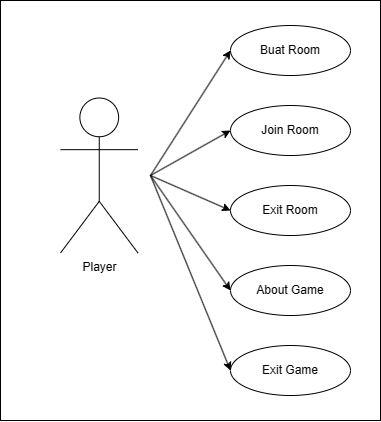
\includegraphics[width=10cm]{case-diagram.png}
        \caption{Use Case Diagram}
        \label{fig:case-diagram}
    \end{figure}

    Gambar \ref{fig:case-diagram} menjelaskan tentang \textit{Use Case Diagram} dimana terdapat satu aktor yaitu pemain, serta 5 \textit{Use Case} yaitu \textit{Buat Room, Join Room, Exit Room, About Game, Exit Game}.
    Pemain dapat menjadi server jika pemain melakukan \textit{use case} buat room dan pemain juga bisa menjadi client jika pemain menggunakan \textit{use case join room}, tetapi jika tidak adanya pemain yang menggunakan \textit{use case} buat room, maka \textit{use case} join room tidak dapat digunakan oleh pemain yang menjadi client.
    \textit{use case exit room} dapat dilakukan oleh pemain yang menjadi server maupun menjadi client, dan hal itu akan menghapus sesi room yang sudah dibuat jika semua pemain menggunakan \textit{use case exit room}. \textit{Use case about game} dapat dilakukan oleh pemain untuk mengetahui tentang \textit{game} yang dimainkan, dan yang terakhir jika pemain ingin meninggalkam \textit{game}, pemain mengunakan \textit{Use case Exit Game.}
    \textit{Activity diagram} adalah diagram yang memodelkan aliran aktivitas pada sistem.
    \item Activity Diagram
    \begin{enumerate}
        \item \textit{Activity Diagram} buat \textit{Room}
        \begin{figure}[h]
           \centering
           \includegraphics[width=10cm]{room-diagram.png}
           \caption{Activity Diagram Create Room}
           \label{fig:croom-case}
       \end{figure}
       \\ Gambar \ref{fig:croom-case} merupakan \textit{Activity Diagram Create Room}. Diawali dengan pemain membuka \textit{game}, sistem akan menampilkan menu \textit{game}, player menekan tombol buat room untuk membuat room yang belum tersedia sebagai server atau pemilk room.
       Pada \textit{activity waiting player} pemilik room akan menunggu player/\textit{client} untuk memasukan room dan memulai \textit{game}.
       \newpage
    \item \textit{Activty Diagram} join \textit{Room}
    \begin{figure}[h]
        \centering
        \includegraphics[width=10cm]{joinroom-diagram.png}
        \caption{Activity Diagram Join Room}
        \label{fig:jroom-case}
    \end{figure}
    \\ Gambar \ref{fig:jroom-case} merupakan \textit{activity diagram join room}. Diawali dengan pemain membuka \textit{game}, kemudian sistem akan menampilkan menu dari \textit{game}, player menekan tombol join room, photon unity akan mencarikan room yang tersedia yang sudah dibuat oleh pemain lain atau bisa mengetikan manual custom port yang terdapat pada pembuat room. Pemain akan terhubung ke server atau room yang tersedia jika room valid.
    \newpage
    \item  \textit{Activity Diagram Exit Room}
    \begin{figure}[h]
        \centering
        \includegraphics[width=10cm]{exitroom-diagram.png}
        \caption{Activity Diagram Exit Room}
        \label{fig:eroom-case}
    \end{figure}
    \\ Gambar \ref{fig:eroom-case} merupakan \textit{activity diagram exit room}. Diawali dengan pemain menekan tombol exit room, sistem akan menampilkan menu utama pada \textit{game}.    
    \item \textit{Activity Diagram About Room}
     \begin{figure}[h]
        \centering
        \includegraphics[width=10cm]{aboutcase-diagram.png}
        \caption{Activity Diagram About Room}
        \label{fig:aroom-case}
    \end{figure}
    \\ Gambar \ref{fig:aroom-case} merupakan \textit{activity diagram about room}. Diawali dengan pemain menekan tombol \textit{about room}. Sistem akan menampulkan isi tentang \textit{game} yang dimainkan.
    \item  \textit{Activity Diagram Exit Game}
    \begin{figure}[h]
        \centering
        \includegraphics[width=10cm]{exitgame-diagram.png}
        \caption{Activity Diagram Exit \textit{game}}
        \label{fig:egame-case}
    \end{figure}
    \\ Gambar \ref{fig:egame-case} merupakan \textit{activity diagram exit game}. Diawali dengan pemain menekan tombol \textit{exit game}. Sistem akan mengeluarkan pemain dari game yang sedang dimainkan.
\end{enumerate}
\end{enumerate}



\subsection{Rancangan \textit{Class Diagram Multiplayer Photon}}
\begin{figure}[h]
   \centering
   \includegraphics[width=10cm]{class-diagram-perancangan.png}
    \caption{Rancangan \textit{class diagram} multiplayer photon}
    \label{fig:class-diagram-game}
\end{figure}

Pada gambar \ref{fig:class-diagram-game} merupakan perancangan sistem multiplayer yang akan diterapkan pada gim.
Class PhotonNetwork dan PunClasses merupakan class yang ada pada library photon.
Class PhotonManager merupakan class yang menampung fungsi untuk menyambungkan ke server, membuat \textit{room} dan bergabung pada \textit{room} yang ada.
Class menu sendiri berfungsi sebagai \textit{interface} pada main menu gim, semua aksi yang ada pada main menu ditampung pada class menu.
CreateObjectP merupakan kelas yang berfungsi untuk membuat map atau \textit{game} object yang diinisialisasi.
PlayerM merupakan kelas yang berfungsi untuk menampung semua pergerakan player seperti pergerakan,darah,menembak, dan kamera.
GameplayMultiP merupakan class yang berfungsi sebagai \textit{gameplay} yang akan dimainkan seperti player, point pada \textit{game} dan respawn pemain saat mati.
Dan KarakterPlayer merupakan class yang berfungsi sebagai inisialisasi player utama.

\subsection{Rancangan \textit{Blok} Diagram Alur \textit{Game} Jak Meuprang}
\begin{figure}[h]
    \centering
    \includegraphics[width=10cm]{blok-diagram-game.png}
    \caption{\textit{Blok Diagram } Jak Meuprang}
    \label{fig:aclass-diagram-game}
\end{figure}

Dapat dilihat pada gambar \ref{fig:aclass-diagram-game} digambarkan alur kerja atau aktivitas sebuah sistem \textit{game} yang dimulai \textit{start game} untuk memulai permainan kemudian menunggu \textit{loading} untuk memasuki permainan, sistem akan menginisialisasi objectnya terlebih dahulu seperti map, senjata dan point.
Jika inisialisasi sudah selesai \textit{game} akan dimulai dan pemain spawn pada saat \textit{game} dimulai, jika pemain bertemu pemain lain dan bertempur akan ditemukan dua kondisi, jika mati pemain akan \textit{respawn} ulang dengan waktu 5 detik, jika pemain memenangkan pertempuran maka pemain mendapatkan point.
Ketika \textit{game} sudah habis waktu makan \textit{game} sudah berakhir dan akan mamasukin akhir \textit{game} permainan.

\newpage
\section{Metode Penelitian}
\noindent

Photon memiliki fitur dan metode sendiri dalam mengelola sebuah \textit{game} multiplayer yang menggunakan \textit{framework}-nya. Untuk mengelola metode yang telah disediakan oleh photon, peniliti mengimplementasikan metode matchmaking pada \textit{game} \textit{multiplayer first person shooter}(fps) untuk mencari roomlist atau create room pada \textit{game} \textit{first person shooter}.
        \begin{figure}[h]
         \centering
         \includegraphics[width=10cm]{flowchart-matchmaking}
         \caption{Flowchart Algoritma Matchmaking}
         \label{fig:algoritmamatmaching}
         \end{figure}

Mengacu pada gambar \ref{fig:algoritmamatmaching}, algoritma membutuhkan daftar \textit{room} yang didapatkan dari \textit{interface} photon \textit{Behavior}. Jika belum ada \textit{room} yang tersedia pada daftar \textit{room}, maka dilakukan fungsi detil dari algoritma matchmaking yaitu SearchRoomMatchmaking(). 


        \section{Teknik Pengujian}
        \subsection{Blackbox}
Teknik pengujian yang digunakan yaitu blackbox. Pengujian Black Box pada fungsional sistem yang terdapat pada aplikasi permainan \textit{first person shooter}.

    \begin{table}[h]
    \centering
    \caption{Tabel Pengujian Black Box}
    \label{lab:tabel-pengujian}
    \begin{tabular}{|l|l|l|l|}
    \hline
    \multicolumn{1}{|c|}{NO} & \multicolumn{1}{c|}{Aktivitas Pengujian} & \multicolumn{1}{c|}{Hasil yang diharapkan} & \multicolumn{1}{c|}{Kesimpulan} \\ \hline
    1                        & Tombol Buat Room                         & Membuka panel "Room Panel"                 &                                 \\ \hline
    2                        & Tombol Cari Room                         & Membuka panel "Lobby Panel"                &                                 \\ \hline
    3                        & Tombol Exit Room                         & Kembali ke menu utama                      &                                 \\ \hline
    4                        & Tombol About Game                        & Menampilkan popup about game               &                                 \\ \hline
    5                        & Tombol exit game                         & Keluar dari aplikasi game                  &                                 \\ \hline
    \end{tabular}
    \end{table}
\newpage        
% \subsection{Pengujian performa jaringan}
% Teknik pengujian performa untuk melakukan pengujian jaringan pada photon cloud menggunakan wireshark qos untuk mengukur troughput, delay dan packet loss.
\section{Hasil yang diharapkan}
Hasil yang diharapkan pada penilitian ini antara lain :
\begin{enumerate}
    \item Keberhasilan dalam mengetahui kelayakan aplikasi \textit{game} dengan metode \textit{blackbox testing}, dan pengujian performa jaringan.
    \item Keberhasilan \textit{game} terhubung dengan unity python networking yang dapat dimainkan secara multiplayer online.
    \item Laporan tugas akhir mahasiswa jurusan Teknologi Informasi Dan Komputer.
\end{enumerate}
\chapter{HASIL DAN PEMBAHASAN}
\section{Hasil}
\noindent

Tahapan ini merupakan tahapan yang berisi tentang penjelasan bagaimana game ini dapat bekerja sesuai dengan yang diharapkan dan dapat berjalan dengan baik. Tahapan ini meliputi perancangan perangkat lunak, bagian program yang penting dan implementasi sehingga dapat dipahami dengan baik dan mengetahui cara menggunakannya.

\subsection{Desain Perangkat Lunak}

\begin{enumerate}
    \item Tampilan \textit{Connecting Network} \\
    Tampilan \textit{connecting network} adalah tampilan awal disaat game dibuka, pada tampilan ini akan menghubungkan player ke jaringan photon .
    \begin{figure}[h]
        \centering
        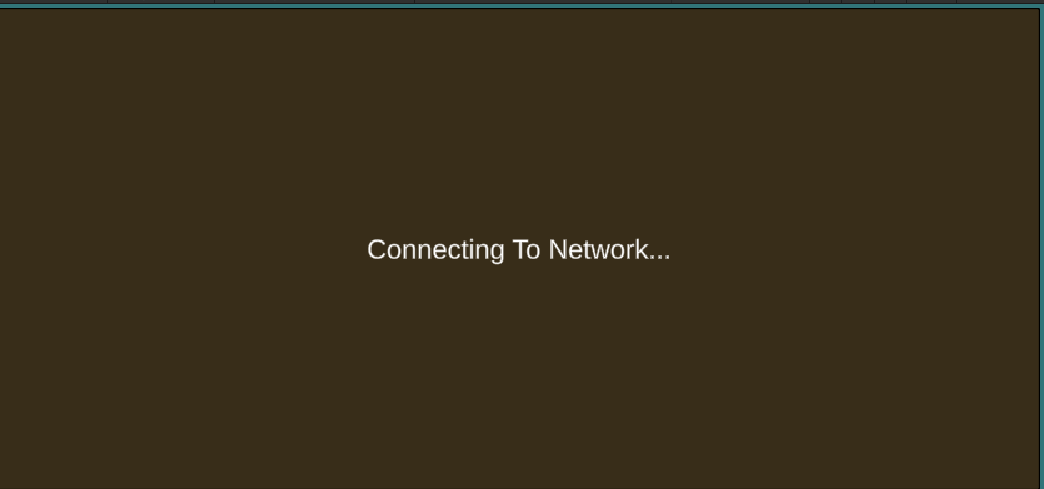
\includegraphics[width=10cm]{connecting.png}
        \caption{Tampilan \textit{Connecting Network}}
        \label{fig:connecting}
    \end{figure}
    \item Tampilan Set \textit{Nickname} \\
    Set \textit{nickname menu} merupakan letak dimana player harus mengisikan nama untuk memberikan identitas nama dari player. 
    \newpage
    \begin{figure}[h]
        \centering
        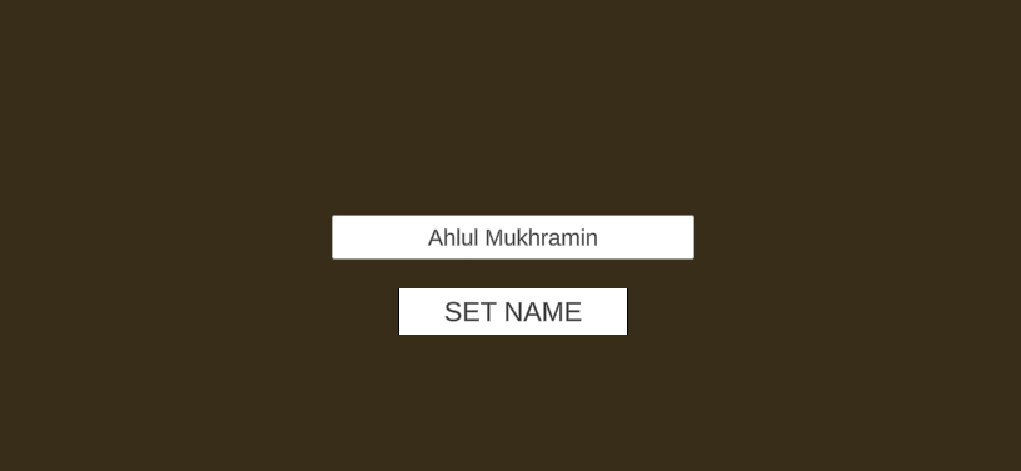
\includegraphics[width=10cm]{setnama.png}
        \caption{Tampilan Mengatur Nama}
        \label{fig:setnama}
    \end{figure}
    \item Tampilan Menu Utama\\
    Tampilan menu utama adalah tampilan menu yang terdapat button "cari room" untuk mencari room yang tersedia, "buat room" untuk membuat room sebagai master room,  "thanks to" untuk melihat \textit{credit} asset yang digunakan dan "Keluar" untuk menutup game.
    \begin{figure}[h]
        \centering
        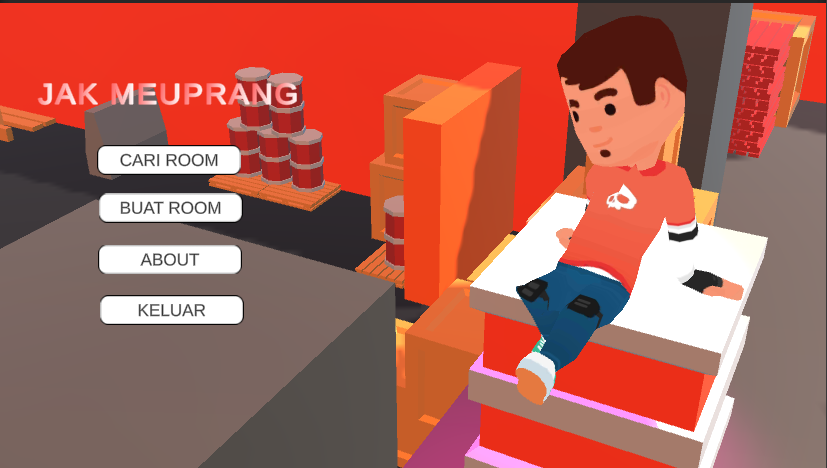
\includegraphics[width=10cm]{menuutama.png}
        \caption{Tampilan Menu Utama}
        \label{fig:menutama}
    \end{figure}
    \item Tampilan Pencarian Room\\
    Pencarian room merupakan menu untuk mencari room yang tersedia yang dibuat oleh player lain untuk memainkan game bersama.
    \newpage
    \begin{figure}[h]
        \centering
        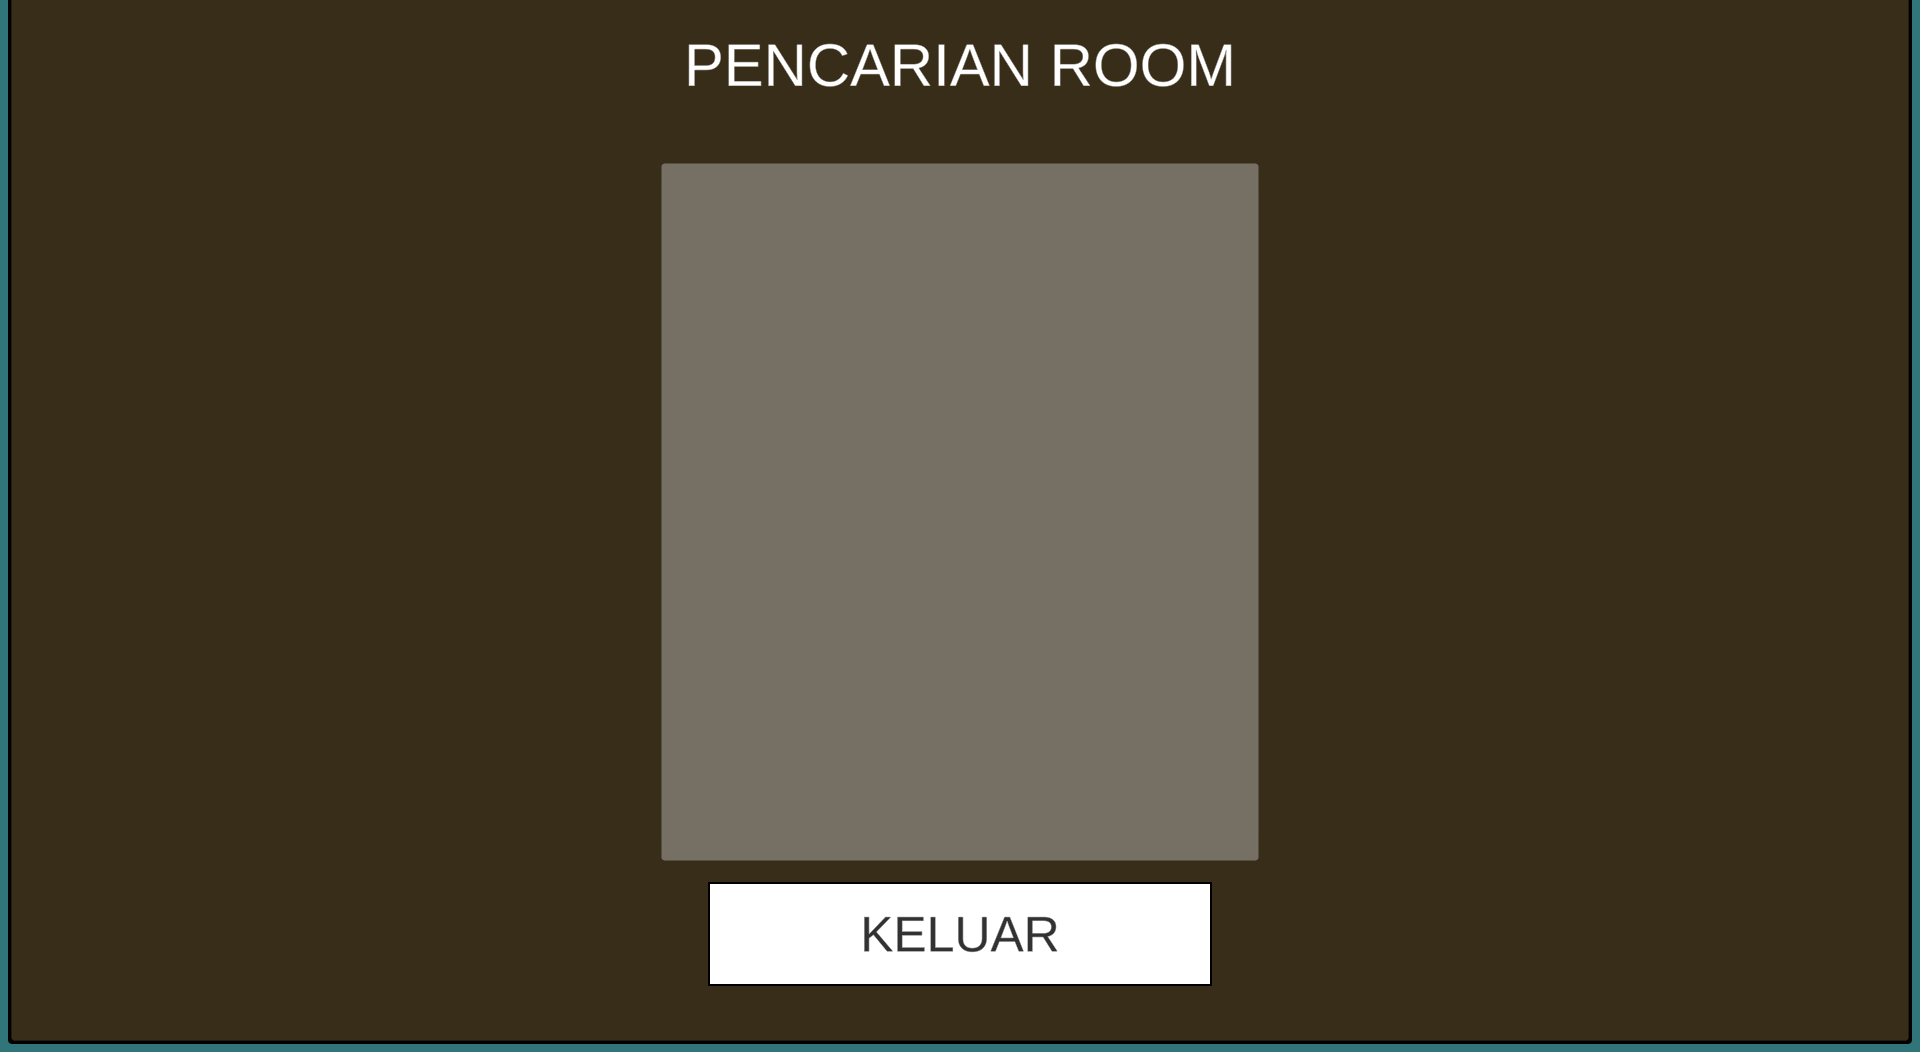
\includegraphics[width=10cm]{pencarian.png}
        \caption{Tampilan Pencarian}
        \label{fig:pencarian}
    \end{figure}
    \item Tampilan Buat Room \\
    Buat room merupakan menu untuk membuat room bagi player ingin menjadi host pada room tersebut, pada menu buat room ini player harus mengisikan nama room terlebih dahulul seperti gambar \ref{fig:namaroom}.
    \begin{figure}[h]
        \centering
        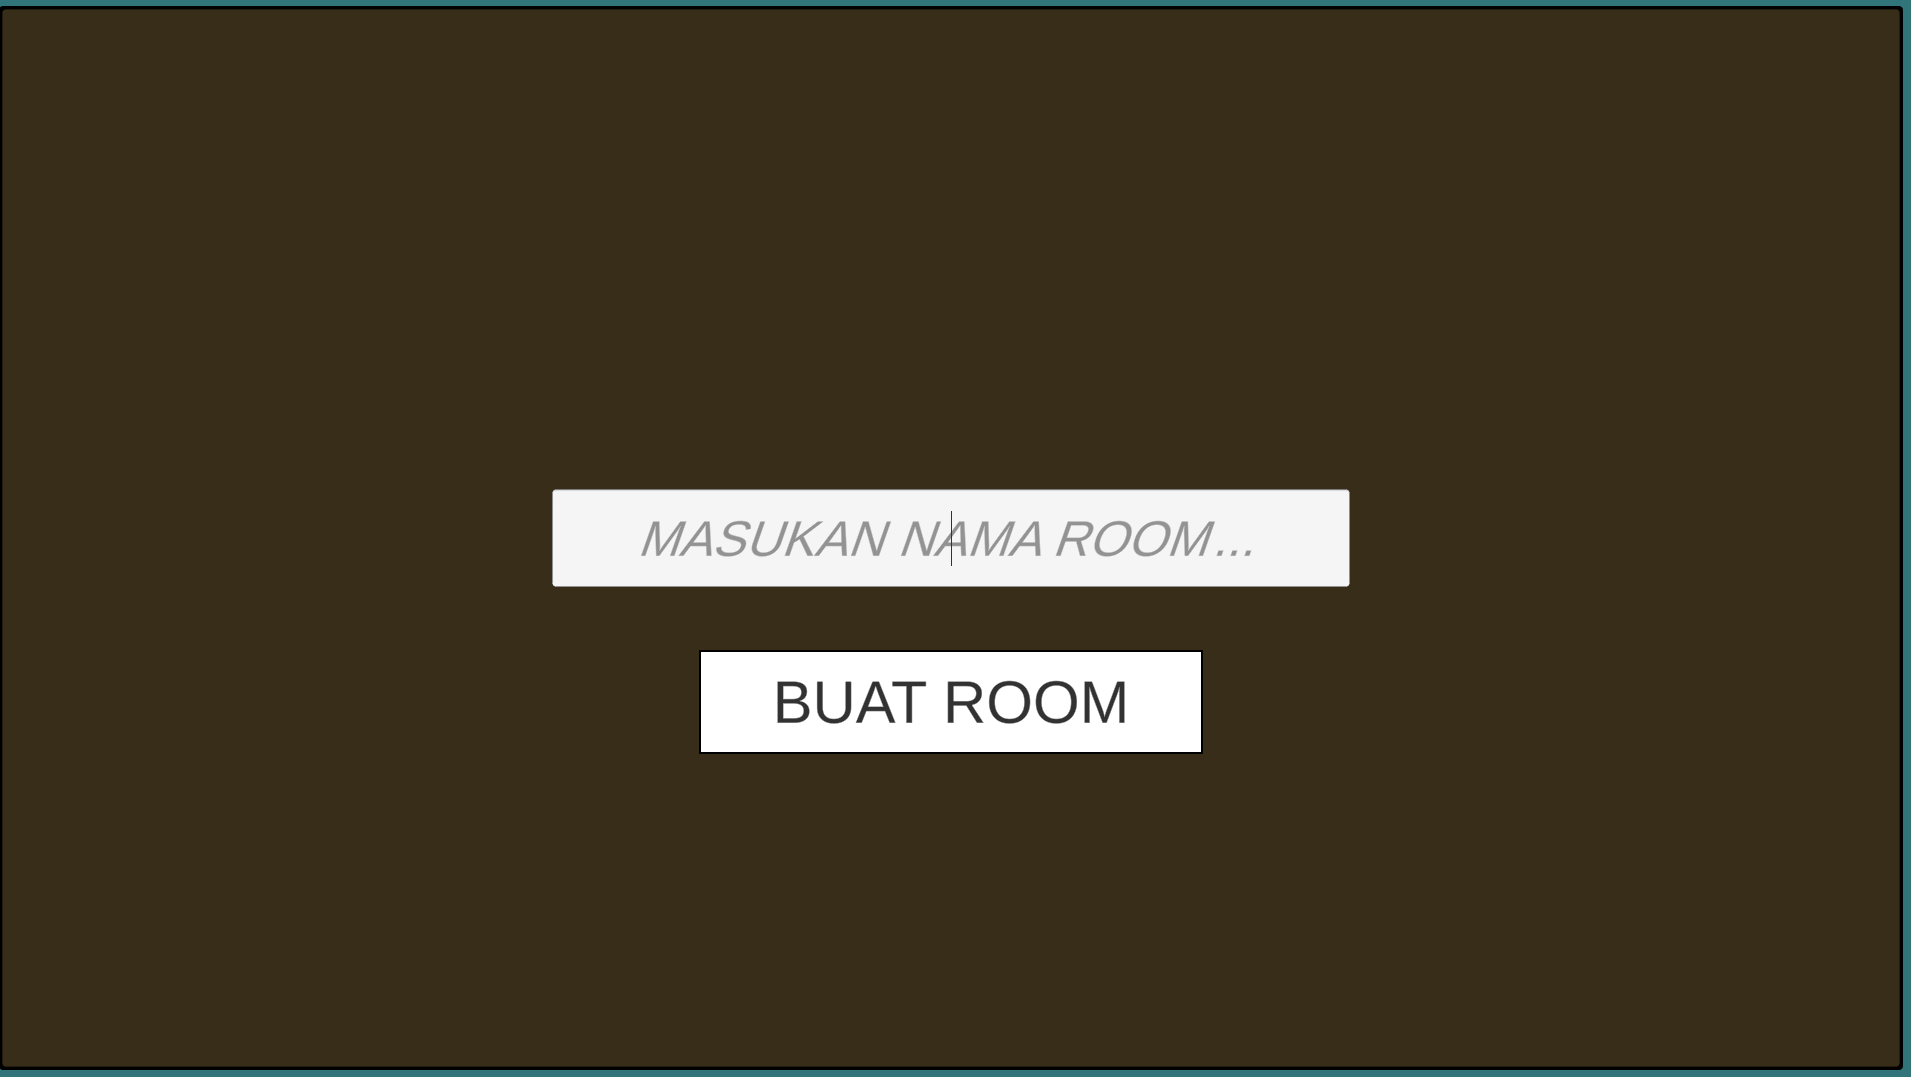
\includegraphics[width=10cm]{namaroom.png}
        \caption{Tampilan Buat Nama Room}
        \label{fig:namaroom}
    \end{figure}
    \\ setelah player telah mengisikan nama room maka akan menampilkan \textit{instance} baru yang berisi player player pada room tersebut, dan hanya host room yang dapat memulai permainannya.
    \newpage
    \begin{figure}[h]
        \centering
        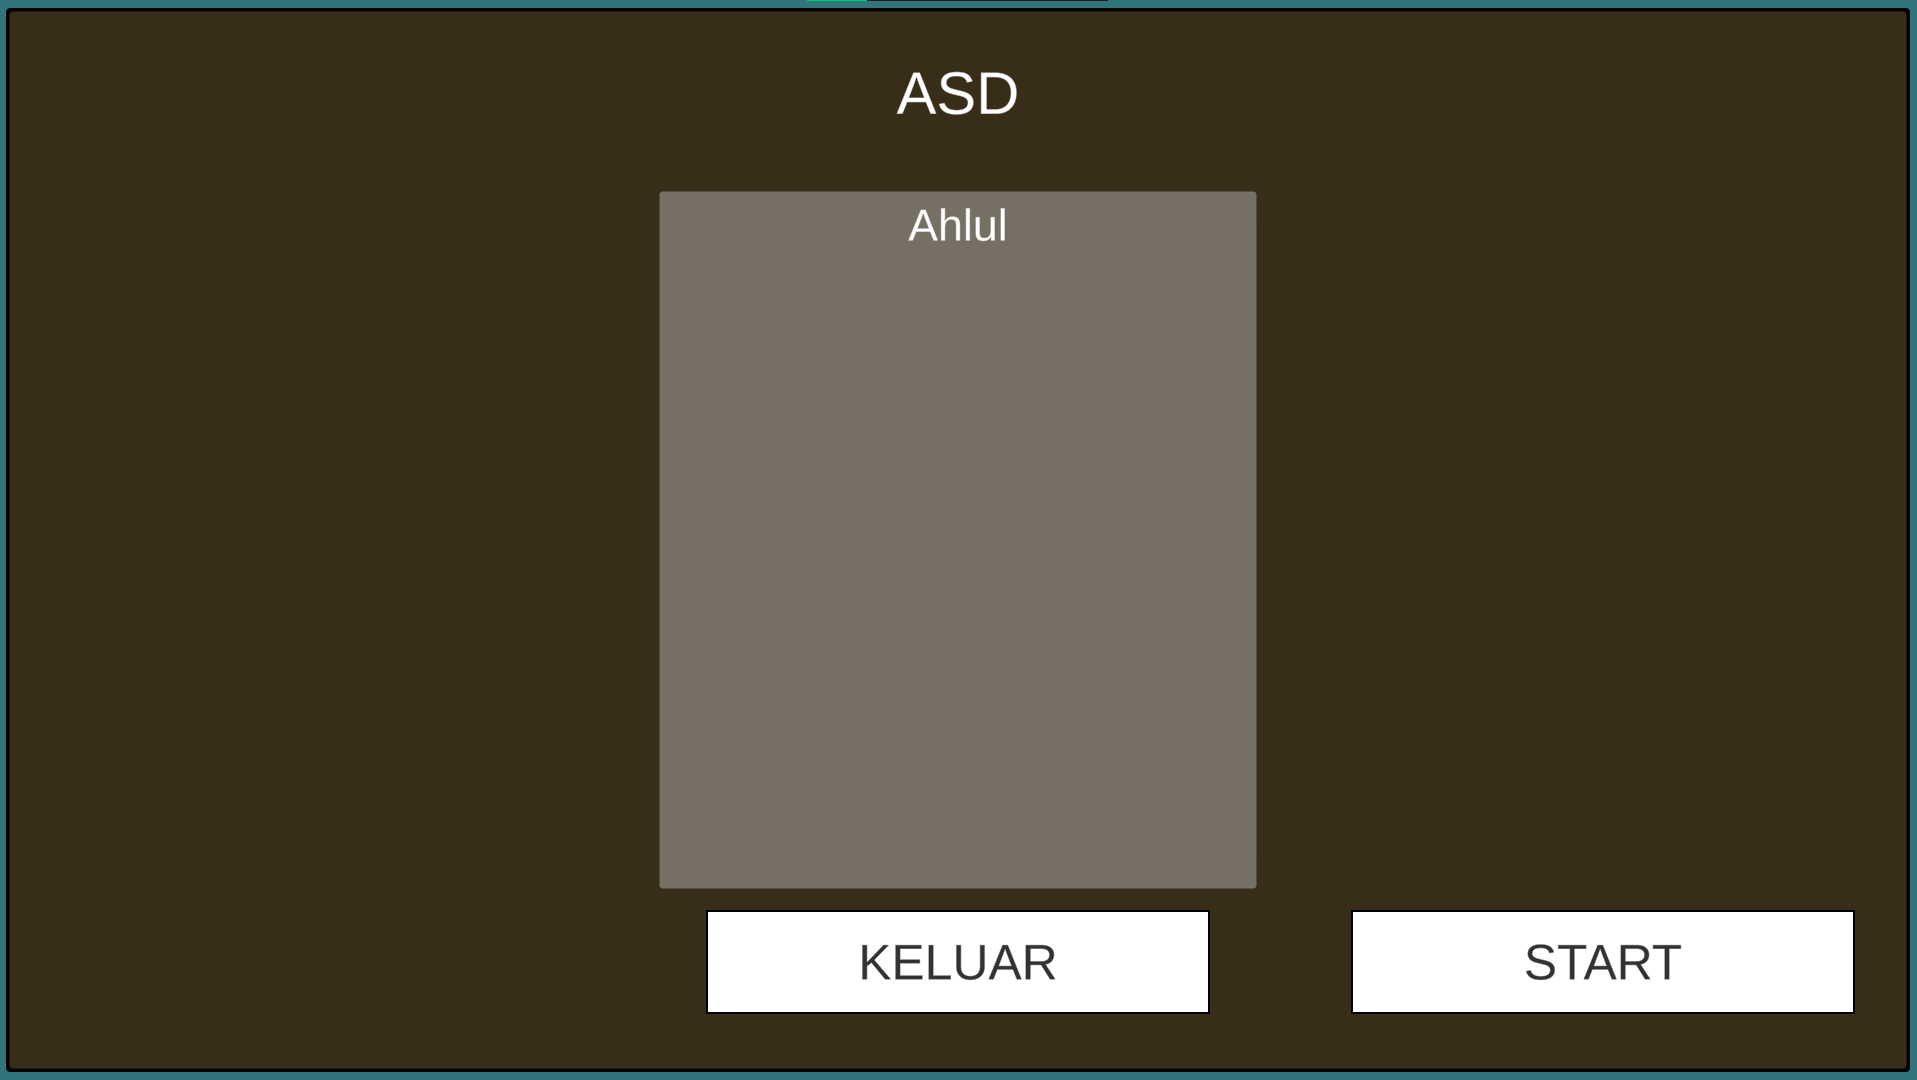
\includegraphics[width=10cm]{roomdone.png}
        \caption{Tampilan Room Telah Dibuat}
        \label{fig:roomdone}
    \end{figure}
    \item Tampilan Credit/About \\
    Tampilan ini merupakan tampilan informasi dari asset asset mana saja yang digunakan sebagai informasi.
    \begin{figure}[h]
        \centering
        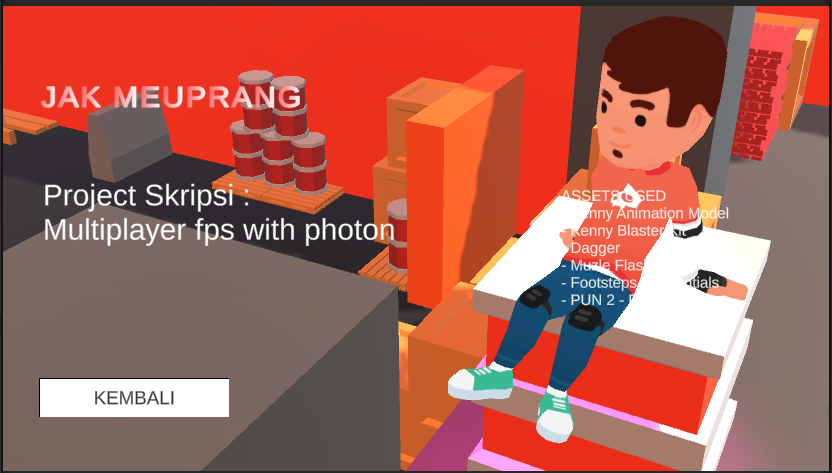
\includegraphics[width=10cm]{thanksto.png}
        \caption{Tampilan About}
        \label{fig:thanksto}
    \end{figure}
    \item Tampilan Gameplay \\
    Tampilan gameplay berisi permainan yang merupakan bagian area gameplay, pada tampilan gameplay ini menampilkan \textit{head up display} (HUD) seperti tampilan health, weapon overheat, player lain dan leaderboard.
    \newpage
    \begin{figure}[h]
        \centering
        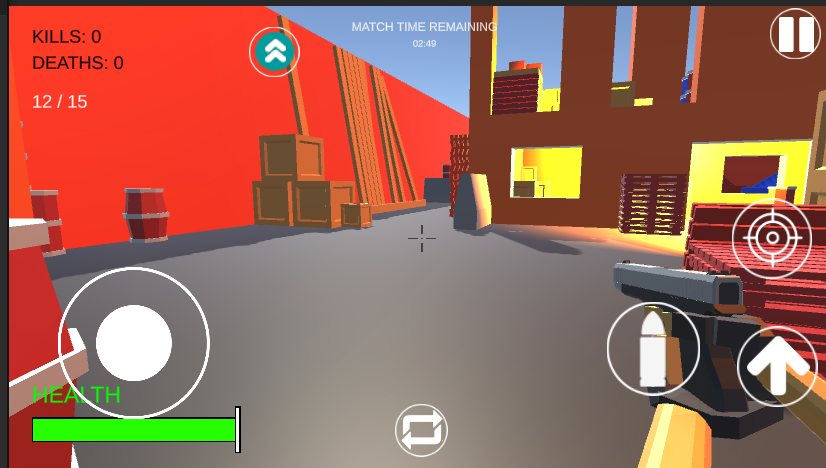
\includegraphics[width=10cm]{gameplay.png}
        \caption{Tampilan Gameplay}
        \label{fig:gameplay}
    \end{figure}
    \item Tampilan Round Over \\
    Tampilan ini ditampilkan jika waktu yang sudah ditentukan habis maka permainan telah berakhir dan player harus keluar untuk membuat room baru.
    \begin{figure}[h]
        \centering
        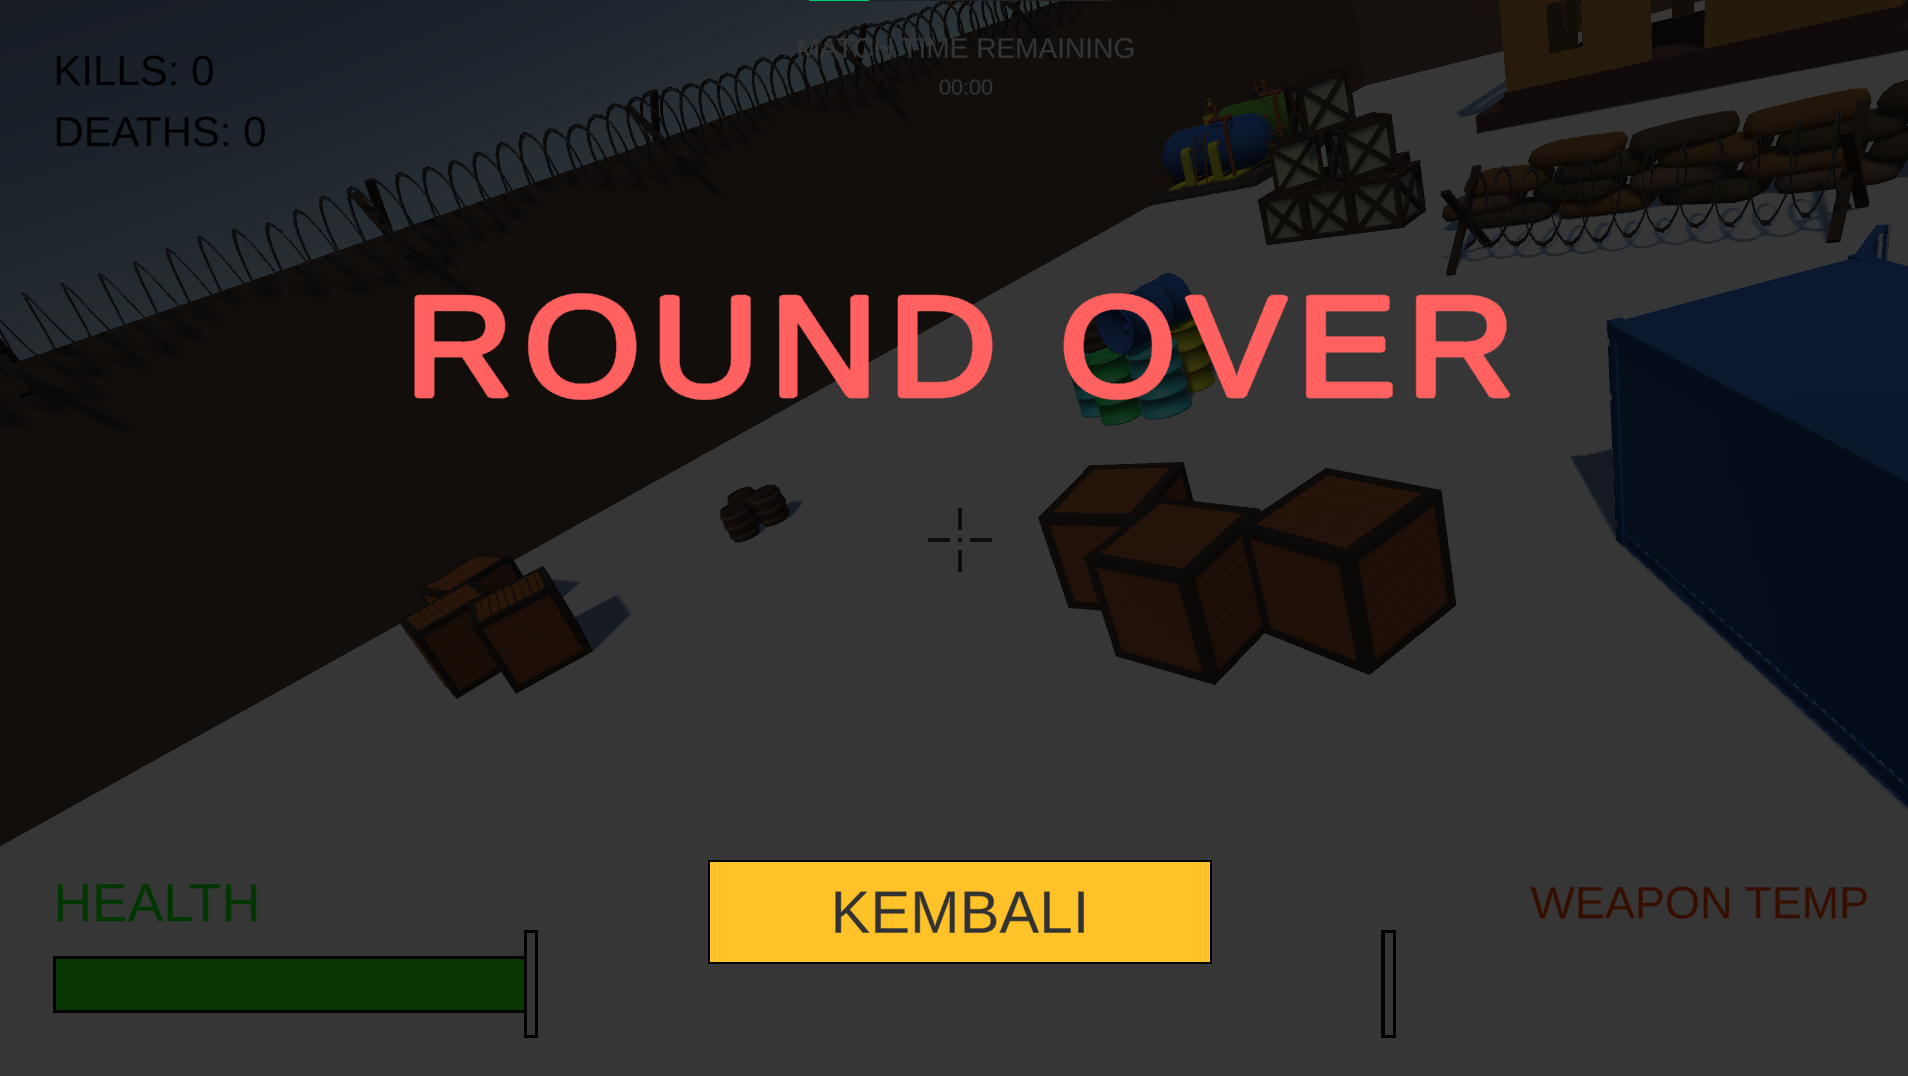
\includegraphics[width=10cm]{roundover.png}
        \caption{Tampilan Round Over}
        \label{fig:roundover}
    \end{figure}
\end{enumerate}

\subsection{\textit{Asset}}
\noindent

Sebuah permainan tidak luput dari berbagai asset karena asset ini adalah bahan bahan yang digunakan pada dalam pembuatan game ini untuk memperbagus tampilan dari game itu sendiri. Asset yang digunakan disini adalah asset gratis dari beberapa platform yang disediakan gratis. Berikut adalah beberapa asset utama yang digunakan dalam pembuatan game "JakMeuprang".

\begin{enumerate}
    \item Karakter \\
    Adapun karakter yang digunakan dalam pembuatan game ini memiliki dua karakter yang memiliki animasi yang sama.
    
    \begin{longtblr}[caption = {\textit{Karakter}}]{
        colspec={Q[valign=b]Q[valign=b]Q[valign=h]},
        row{1}={halign=c},
        vlines,
        hlines,
      }
      No & Gambar & Nama \\
      1 & 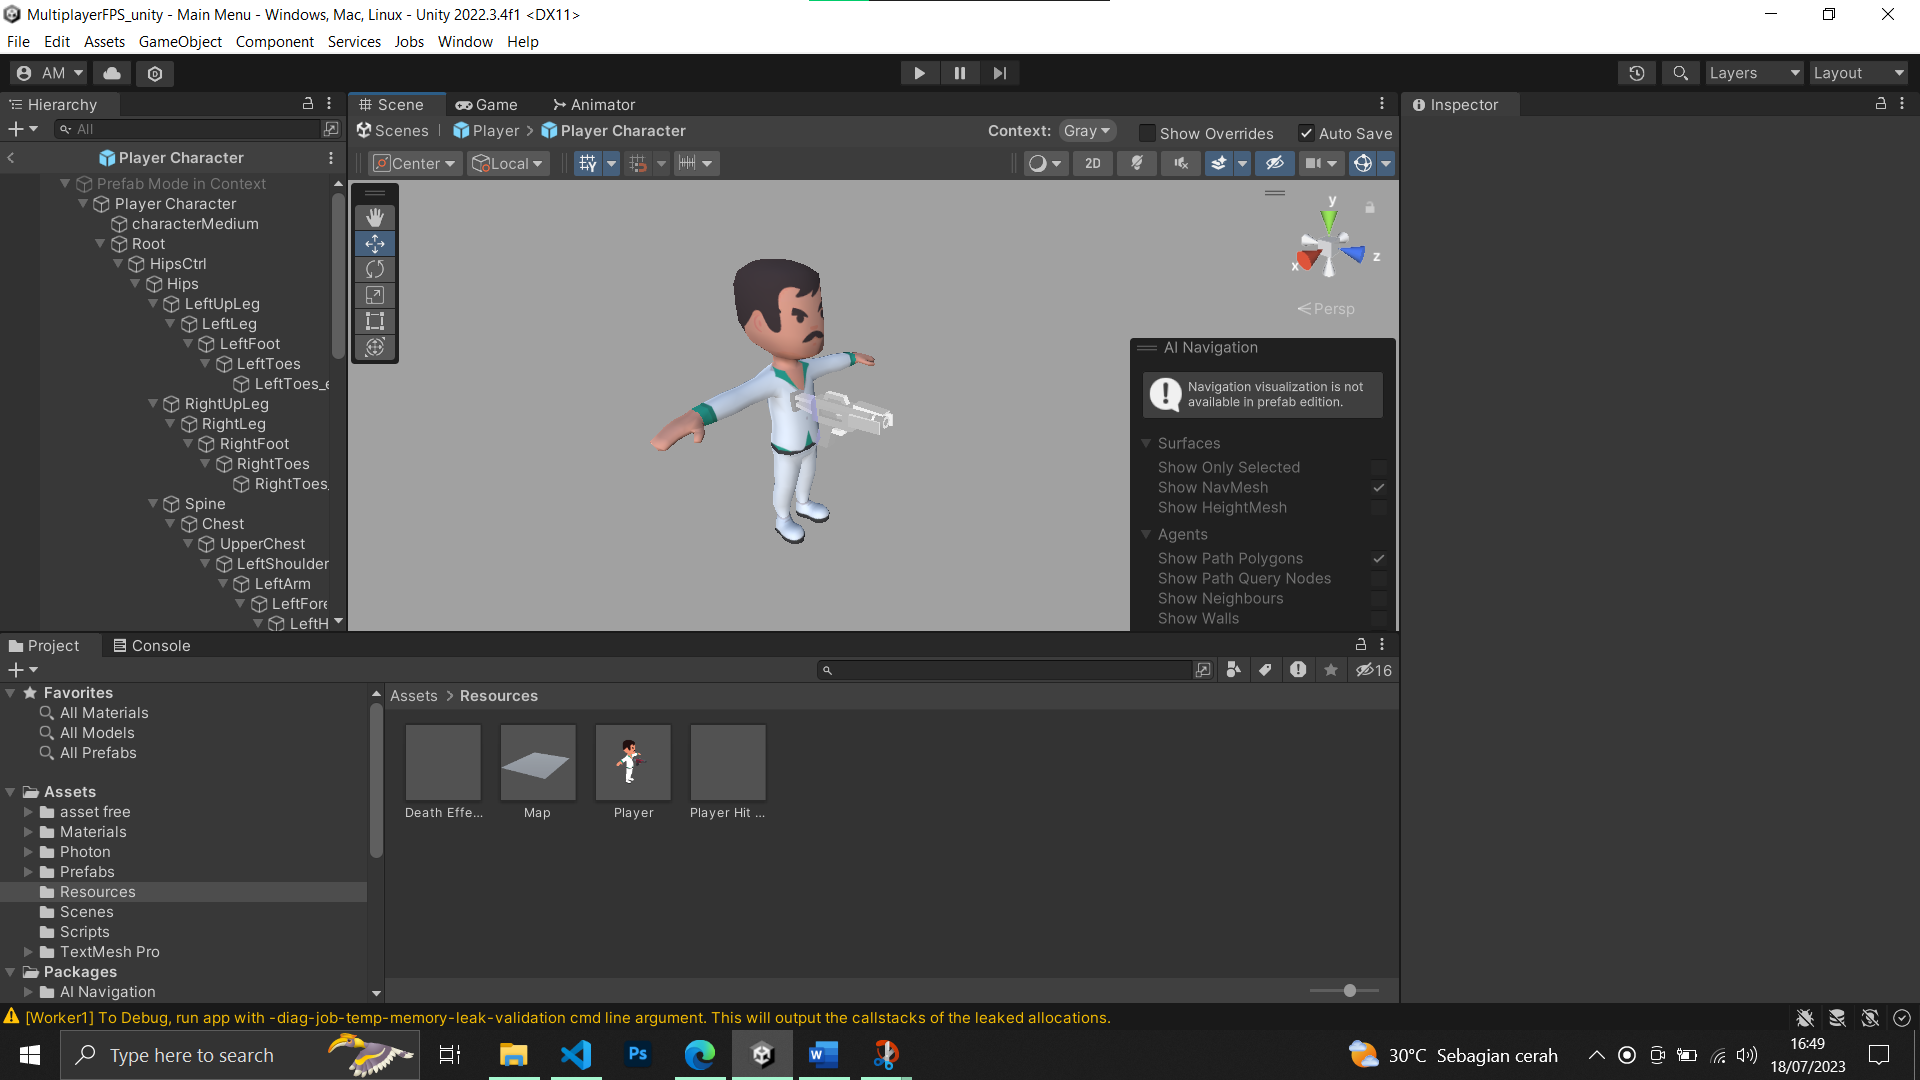
\includegraphics[scale=0.15]{karakter1} & Criminal Karakter \\
      2 & 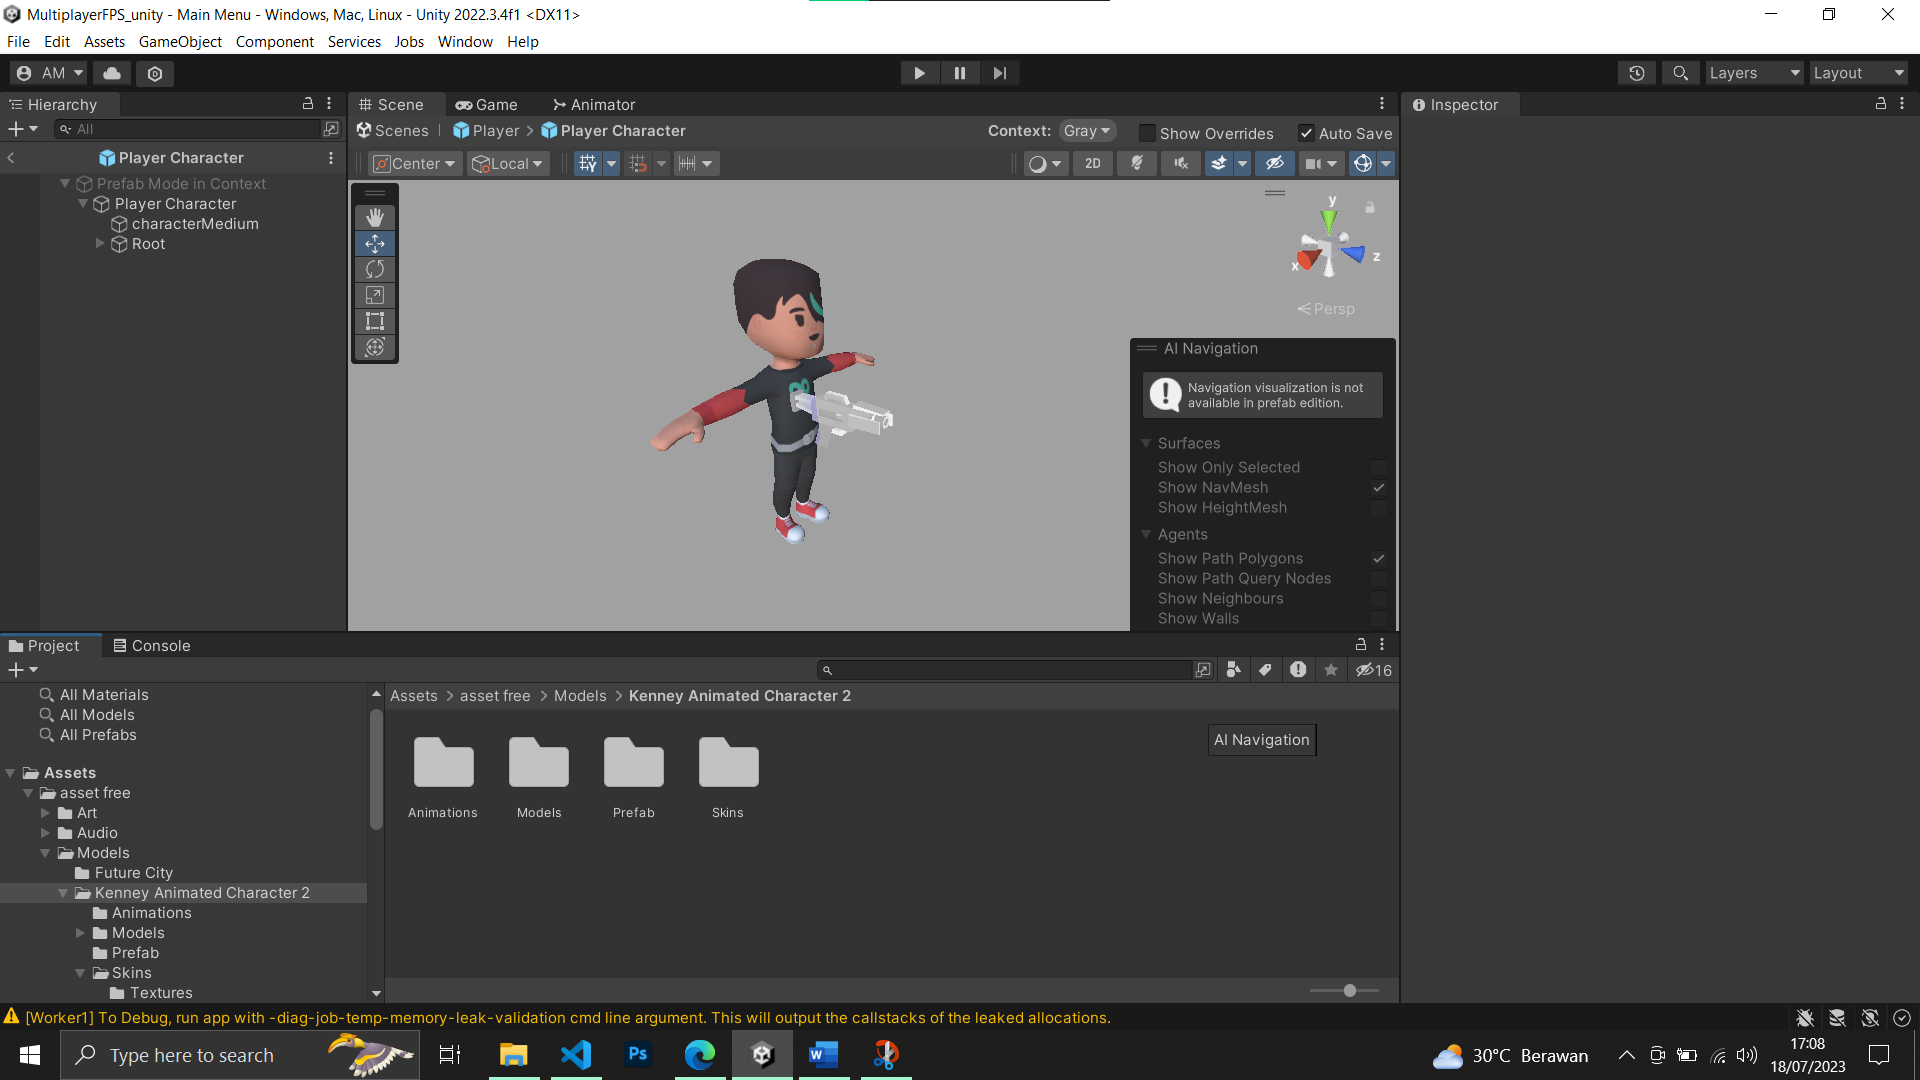
\includegraphics[scale=0.15]{karakter2} & Skater Karakter \\
    \end{longtblr}

    \newpage
    \item Weapon \\
    \begin{longtblr}[caption = {\textit{Karakter}}]{
        colspec={Q[valign=b]Q[valign=b]Q[valign=h]},
        row{1}={halign=c},
        vlines,
        hlines,
      }
      No & Gambar & Nama \\
      1 & 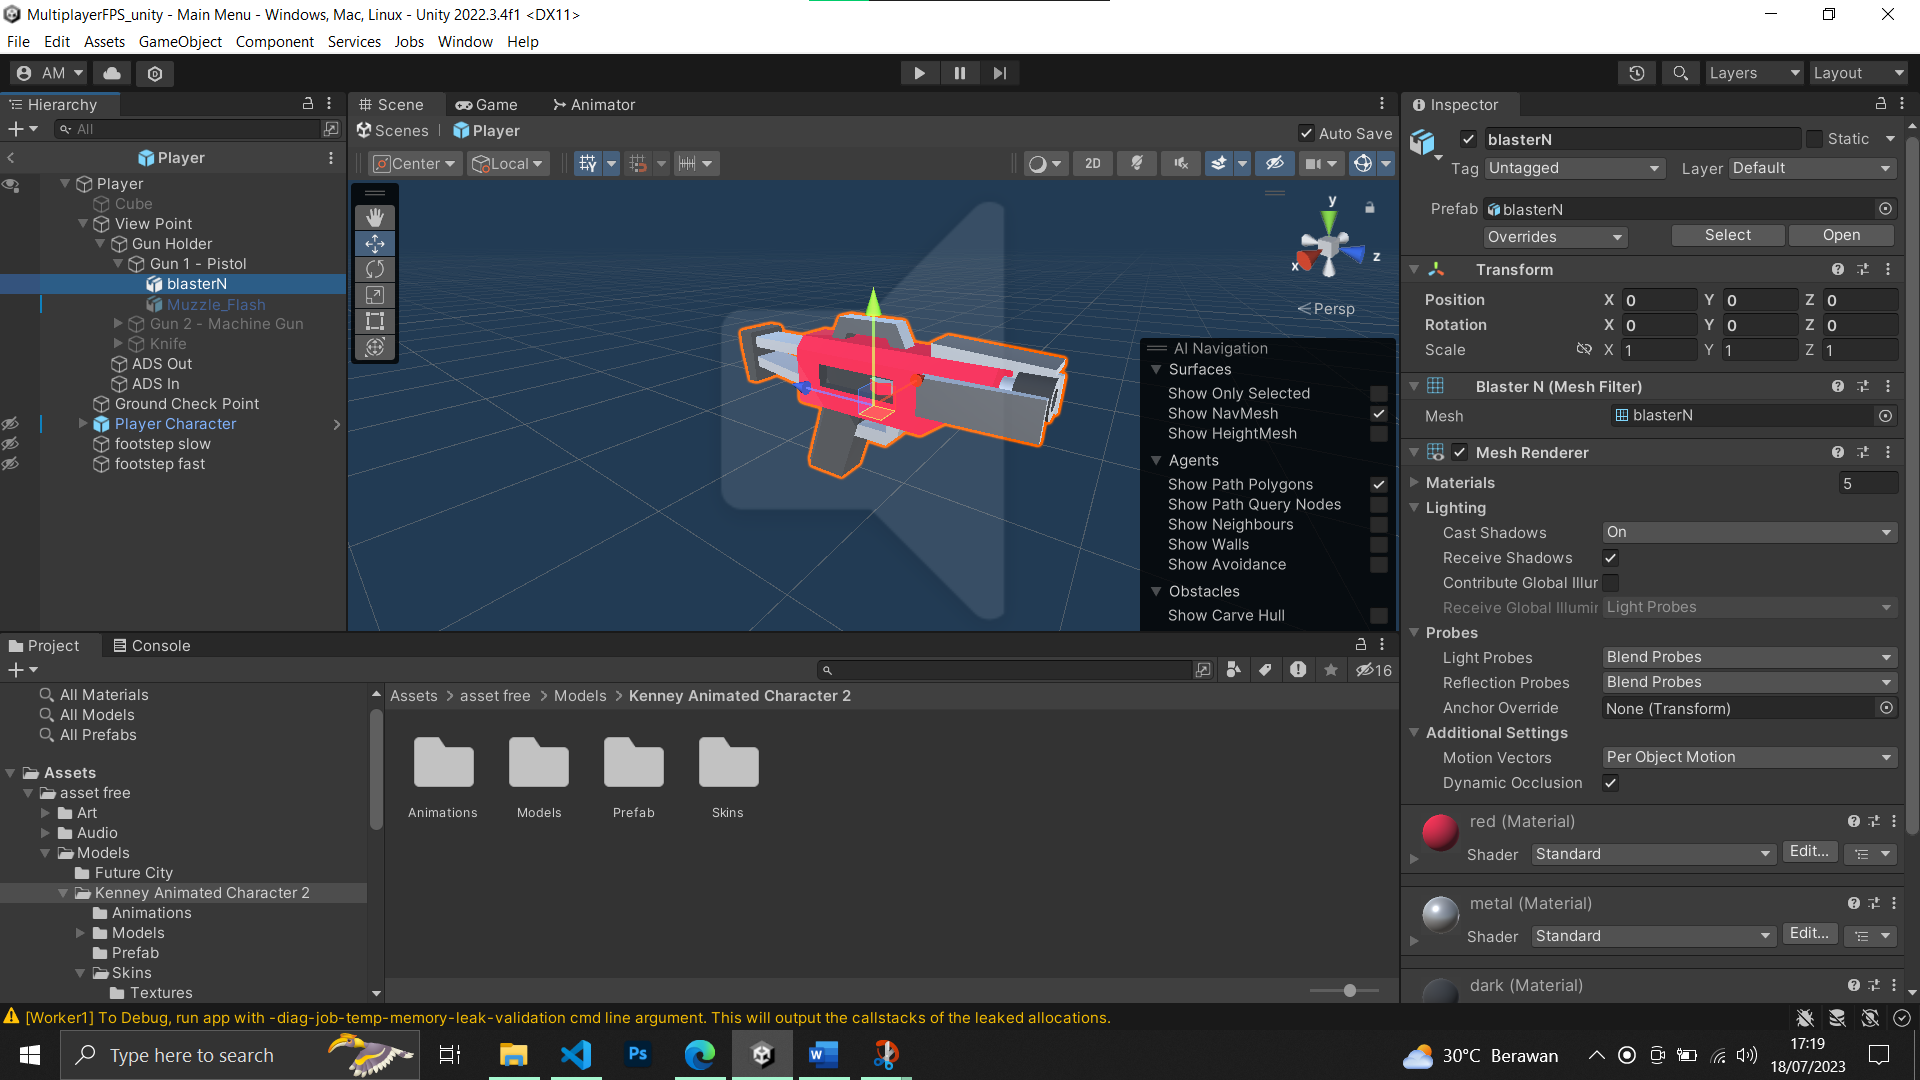
\includegraphics[scale=0.15]{weapon1} & Pistol \\
      2 & 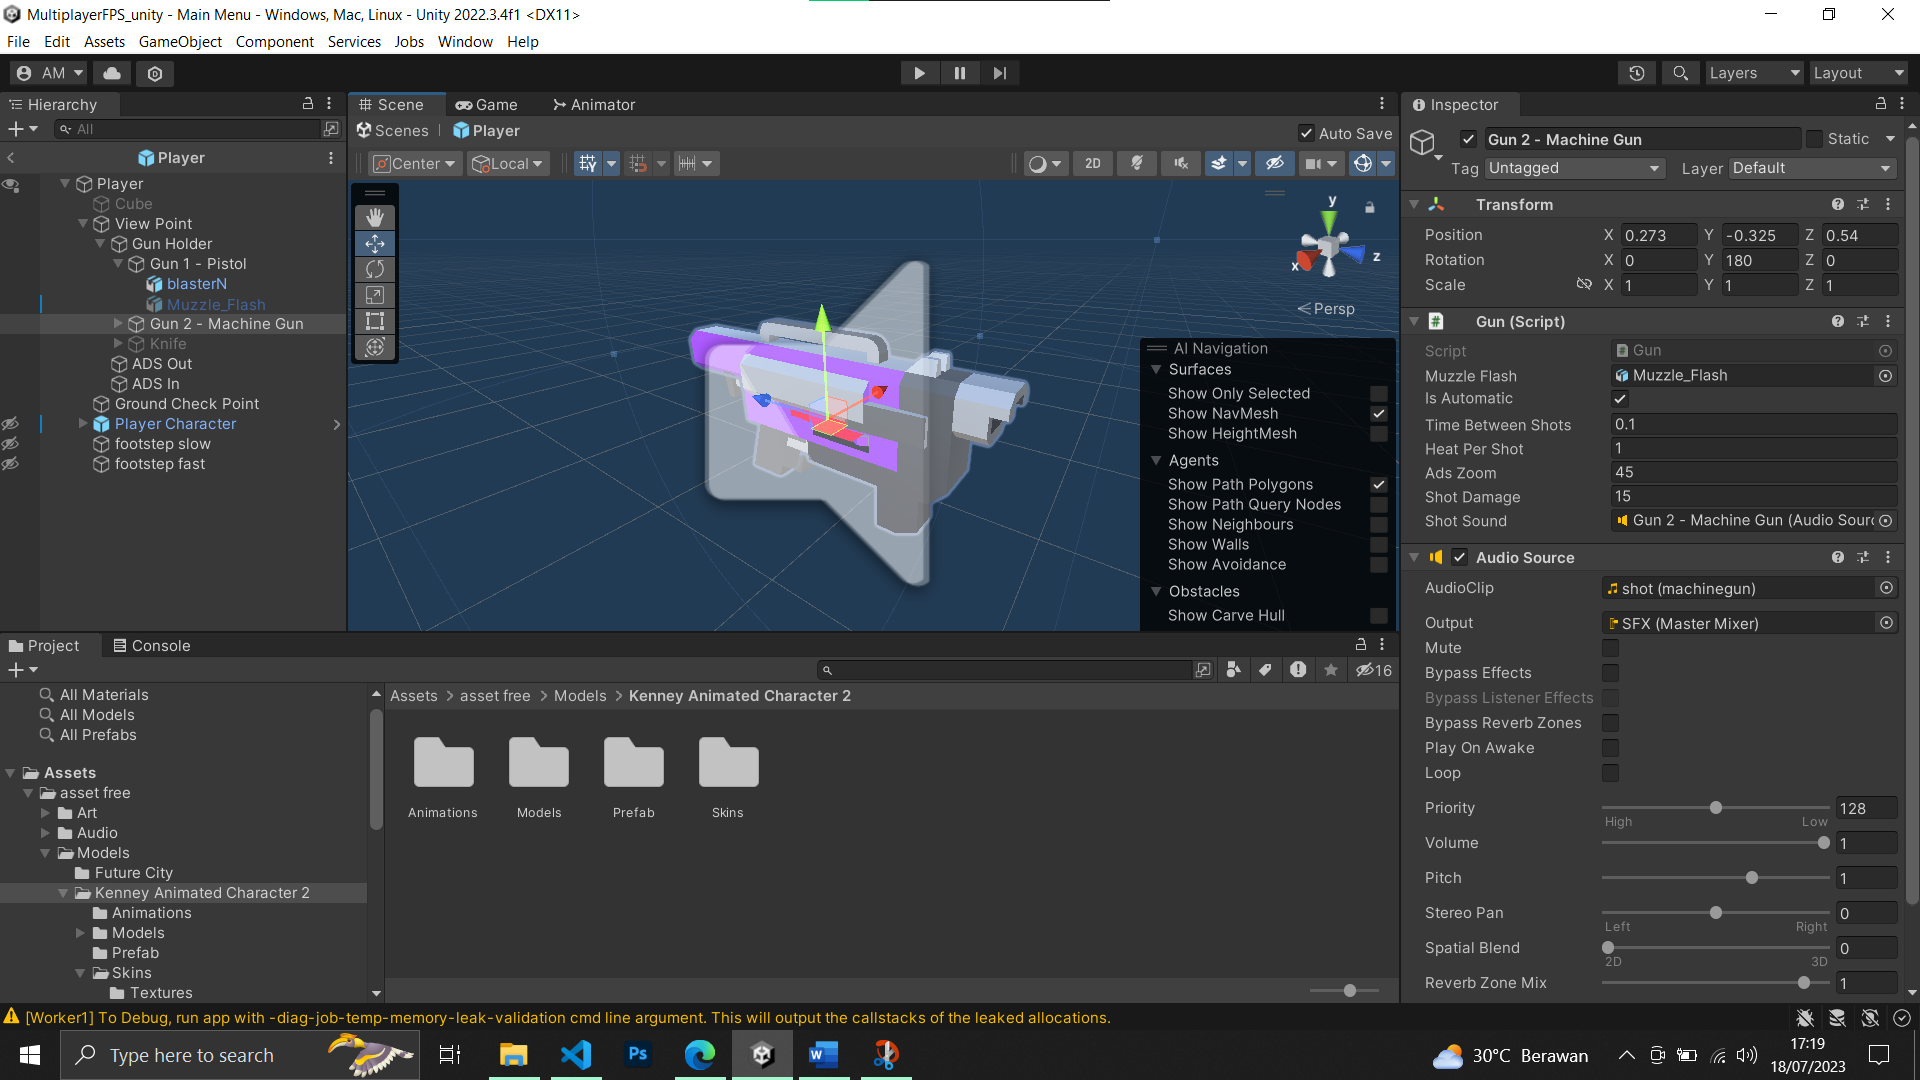
\includegraphics[scale=0.15]{weapon2} & Rifle \\
      2 & 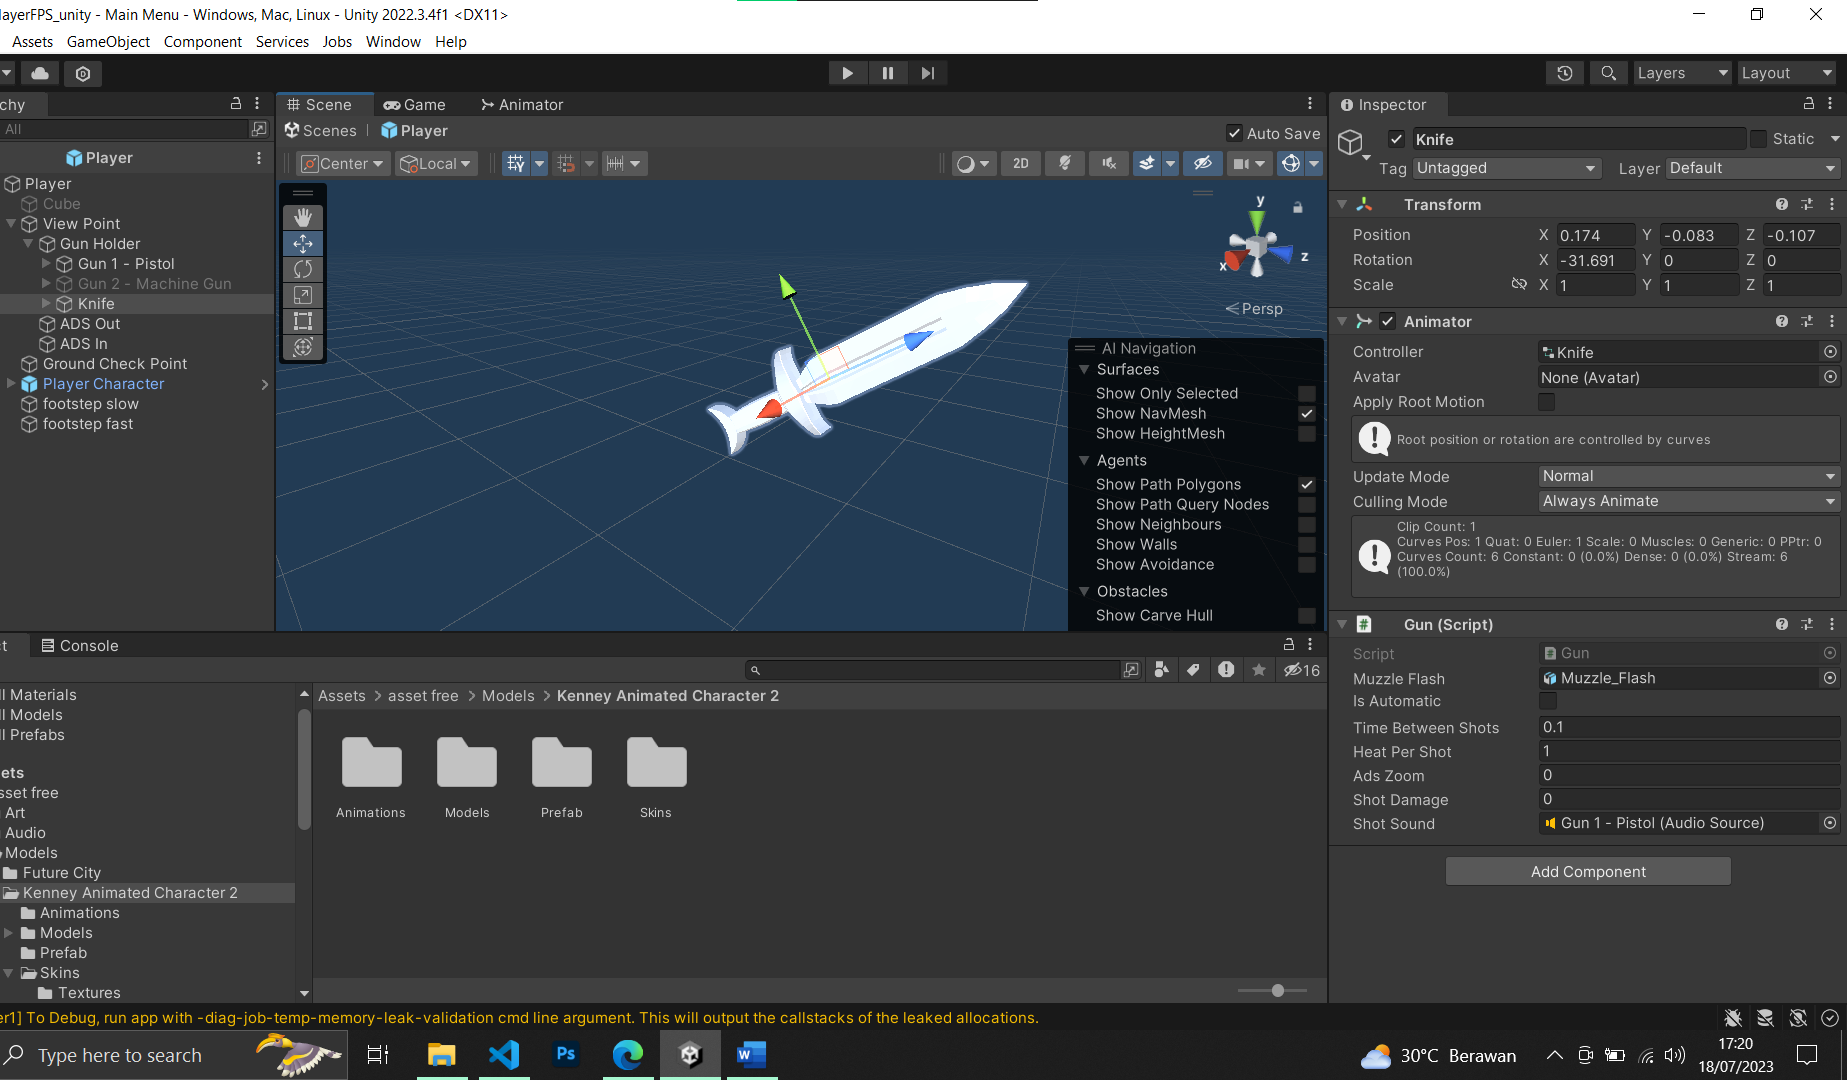
\includegraphics[scale=0.15]{weapon3} & Knife \\
    \end{longtblr}
\end{enumerate}

\section{Pembahasan}
\noindent

Tahap ini merupakan tahap yang berisi penjelasan bagaimana proses game ini dapat bekerja sebagaimana yang diharapkan dan dapat berjalan sesuai rancangan yang telah dibuat. Pada tahap ini meliputi Proses pembuatan game, implementasi photon, gameplay, menu, karakter dan program.
\newpage
\subsection{Proses Pembuatan Game}
\begin{enumerate}
    \item Pembuatan Menu\\
    Tahap pertama adalah membuat menu dimana menu ini akan berinteraksi dengan player.
    \begin{figure}[h]
        \centering
        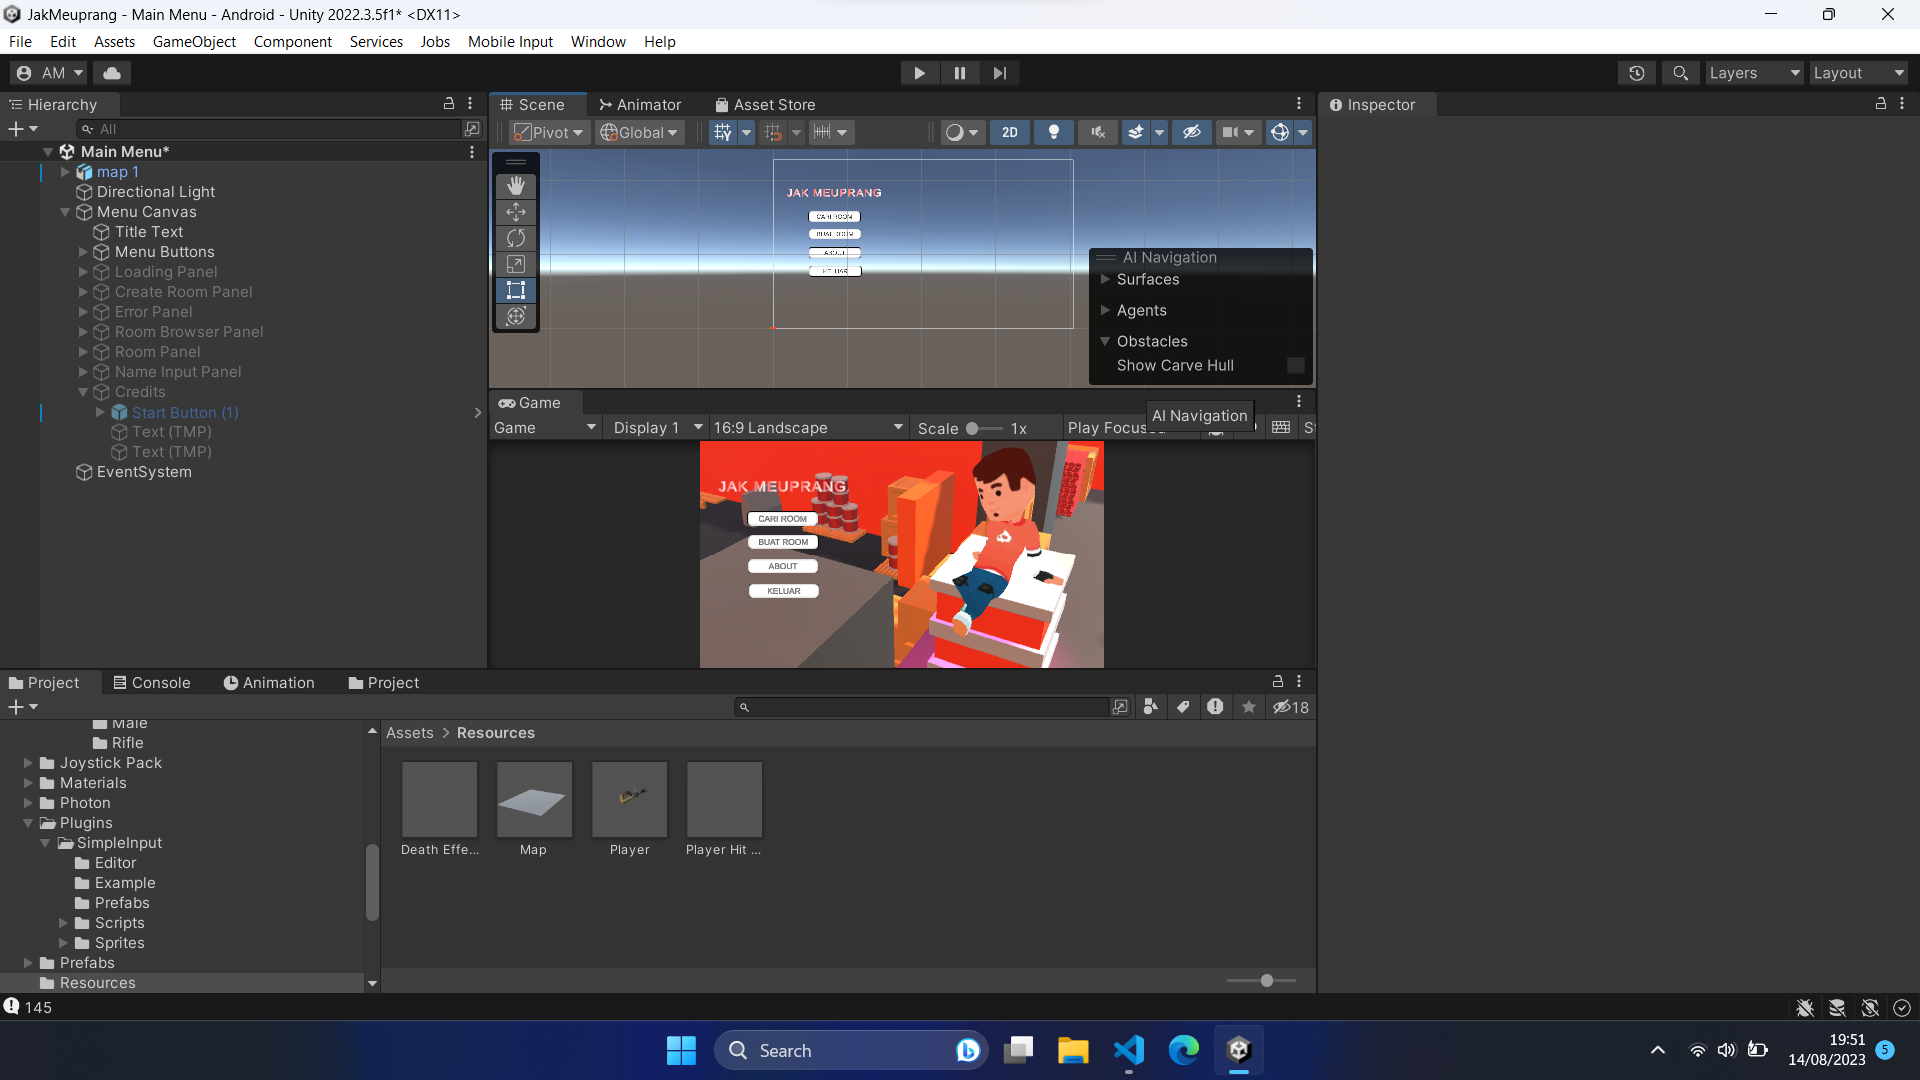
\includegraphics[width=10cm]{pembuatanmenu.png}
        \caption{Tampilan Pembuatan Menu}
        \label{fig:pembuatanmenu}
    \end{figure}
    \item Pembuatan Player Prefabs \\
    Tahap pembuatan player prefabs ini adalah untuk memberikan player dengan karakter yang disediakan menggunakan asset gratis agar dapat digunakan saat bermain.
    \newpage
    \begin{figure}[h]
        \centering
        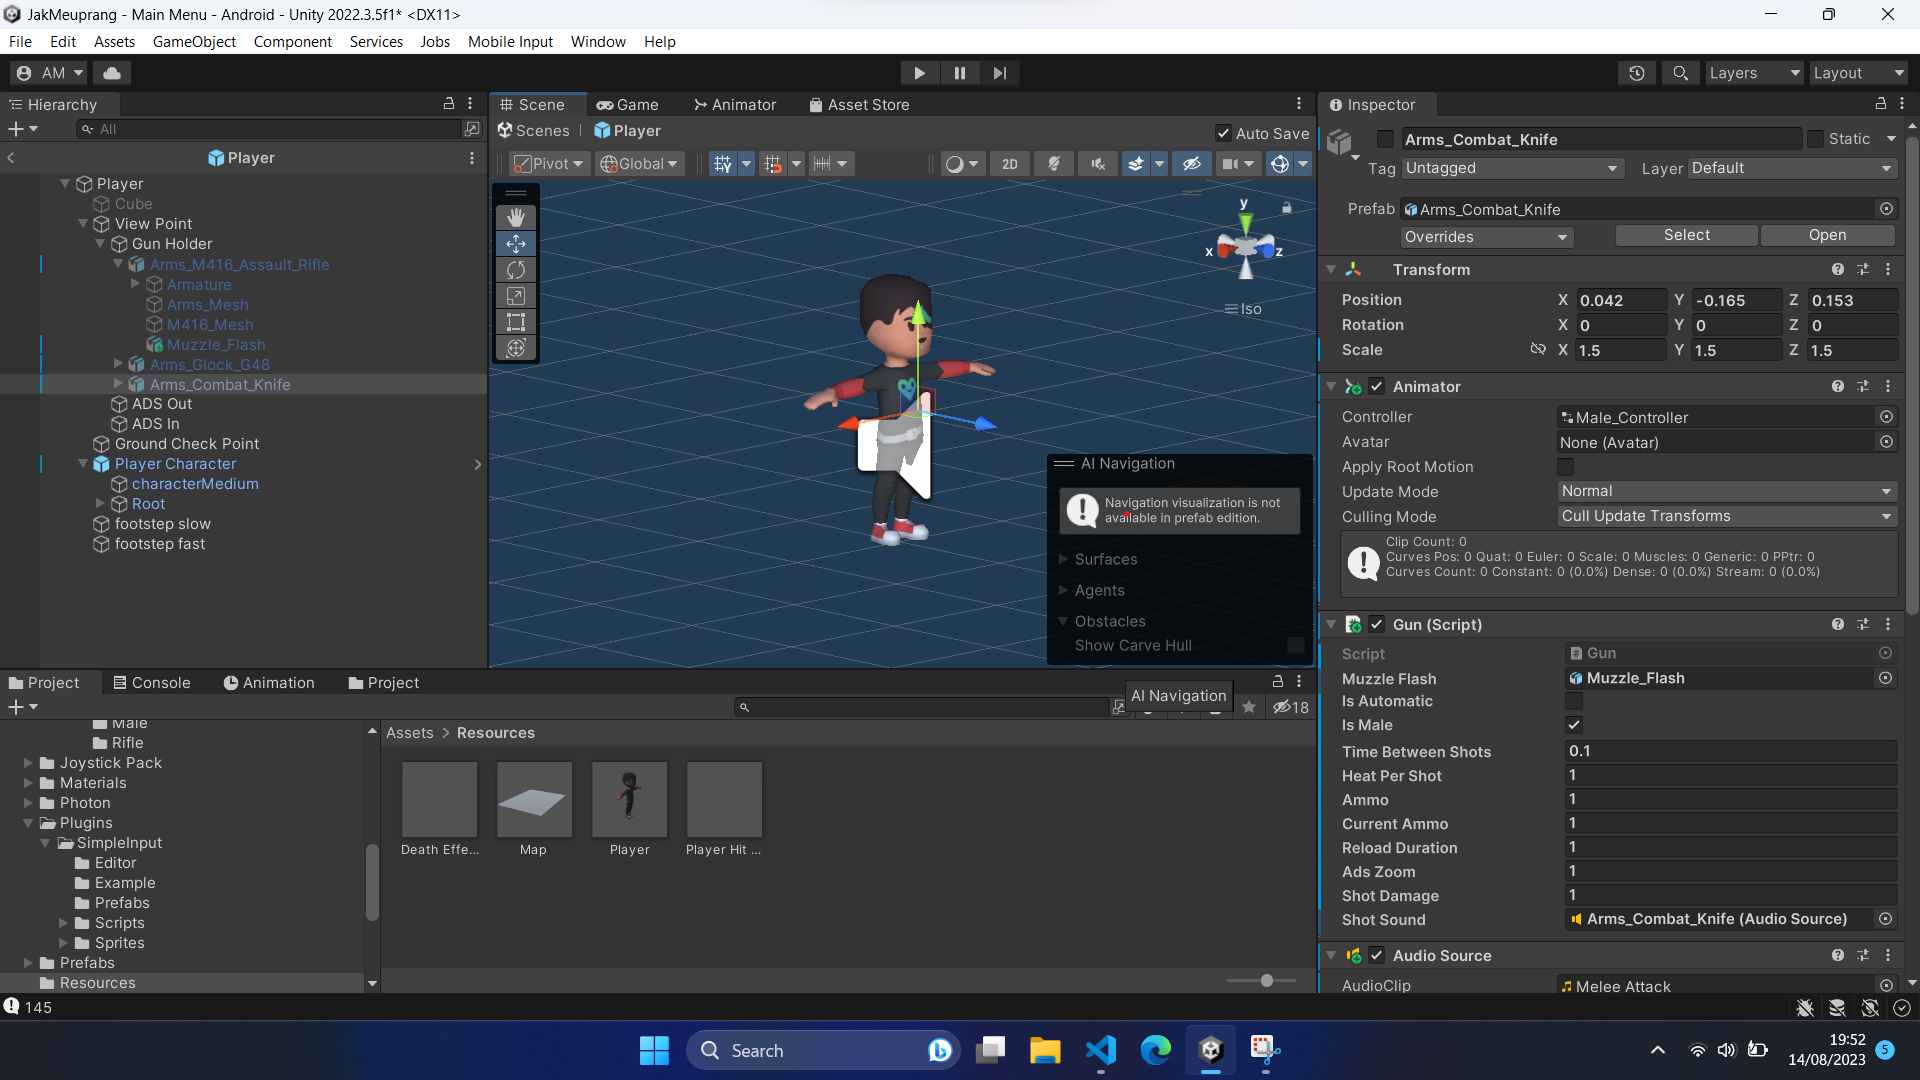
\includegraphics[width=10cm]{pembuatanplayer.png}
        \caption{Tampilan Pembuatan Player}
        \label{fig:pembuatanplayer}
    \end{figure}
    \item Pembuatan Animasi Karakter \\
    Pada tahap ini untuk membuat animasi dari karakter yang disediakan, dari gerakan idle dimana karakter berdiam, walking dimana saat karakter digerakan akan ada animasi berjalan, dan berlari jika inputan dari user terdeteksi berlari akan melakukan animasi berlari.
    \begin{figure}[h]
        \centering
        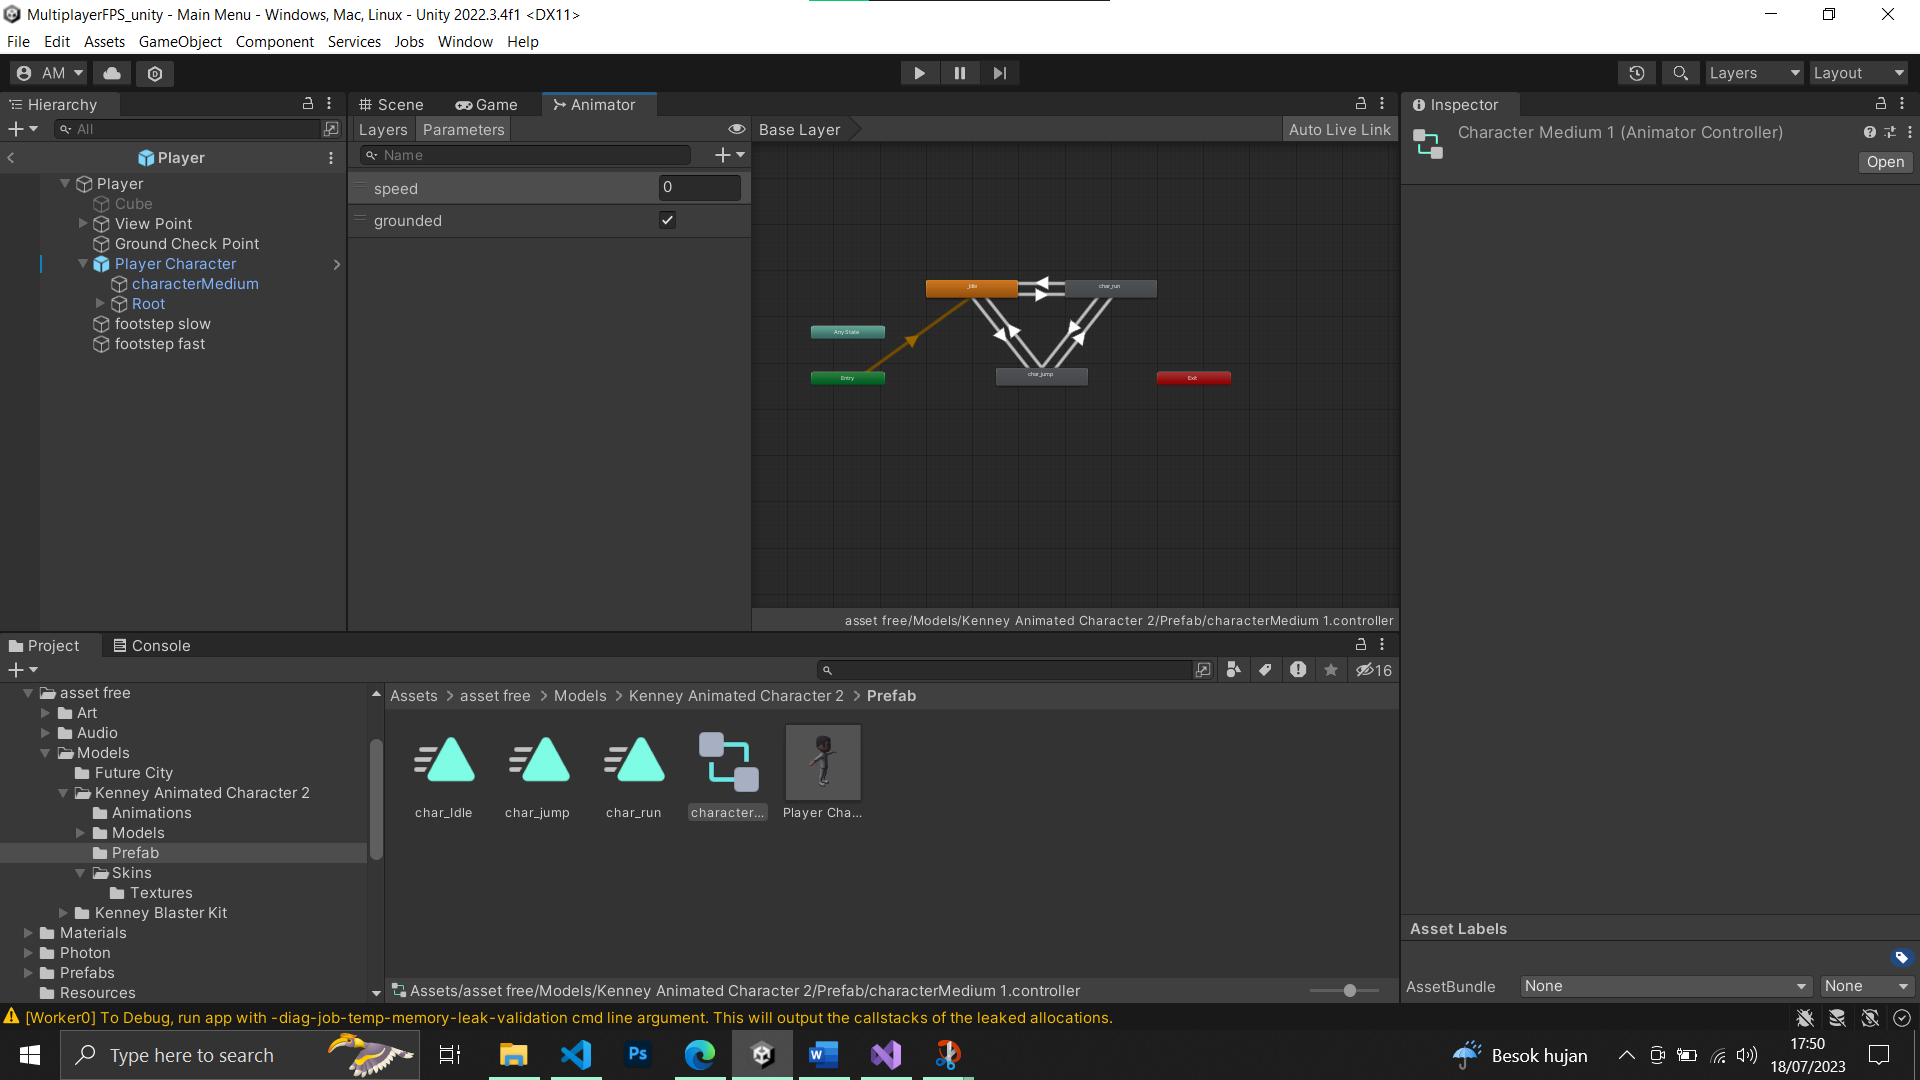
\includegraphics[width=10cm]{pembuatananimasi.png}
        \caption{Tampilan Pembuatan Animasi}
        \label{fig:pembuatananimasi}
    \end{figure}
    \item Objek didalam game \\ 
    Pada tahap ini menjelaskan objek objek yang terdapat saat didalam permainan
    \begin{enumerate}
        \item Weapon\\
        Player mendapatkan 3 senjata yaitu pistol, rifle, pisau.
        \item Health \\
        Player diberikan darah , jika darah berkurang makan player akan terdestroy objectnya.
        \item Weapon Ammo \\
        Player diberikan ammo saat menembak, jika ammo telah habis maka ammo akan auto reload.
    \end{enumerate}
    \item Sound \\
    Pada tahap ini memberikan sound pada beberapa object yaitu :
    \begin{enumerate}
        \item Foot Step Low \\ 
        Memberikan sound saat player sedang berjalan maka menggunakan sound foot step low.
        \item Foot Step Fast \\
        Memberikan sound saat player berlari maka menggunakan sound foot step fast.
        \item Memberikan Sound Senjata \\ 
        Dengan memberikan sound masing masing pada senjata yang digunakan.
    \end{enumerate}
    \item Pembuatan \textit{Mobile Input} \\
    Tahap ini adalah tahap pembuatan \textit{Mobile input} yang berfungsi untuk menerima inputan \textit{button} dari user yang terdapat pada layar user. Inputannya berupa \textit{Shoot}, \textit{Aiming}, \textit{change weapon}, \textit{pause}, \textit{Move player} dan \textit{LeaderBoard input}.
    \newpage
    \begin{figure}[h]
        \centering
        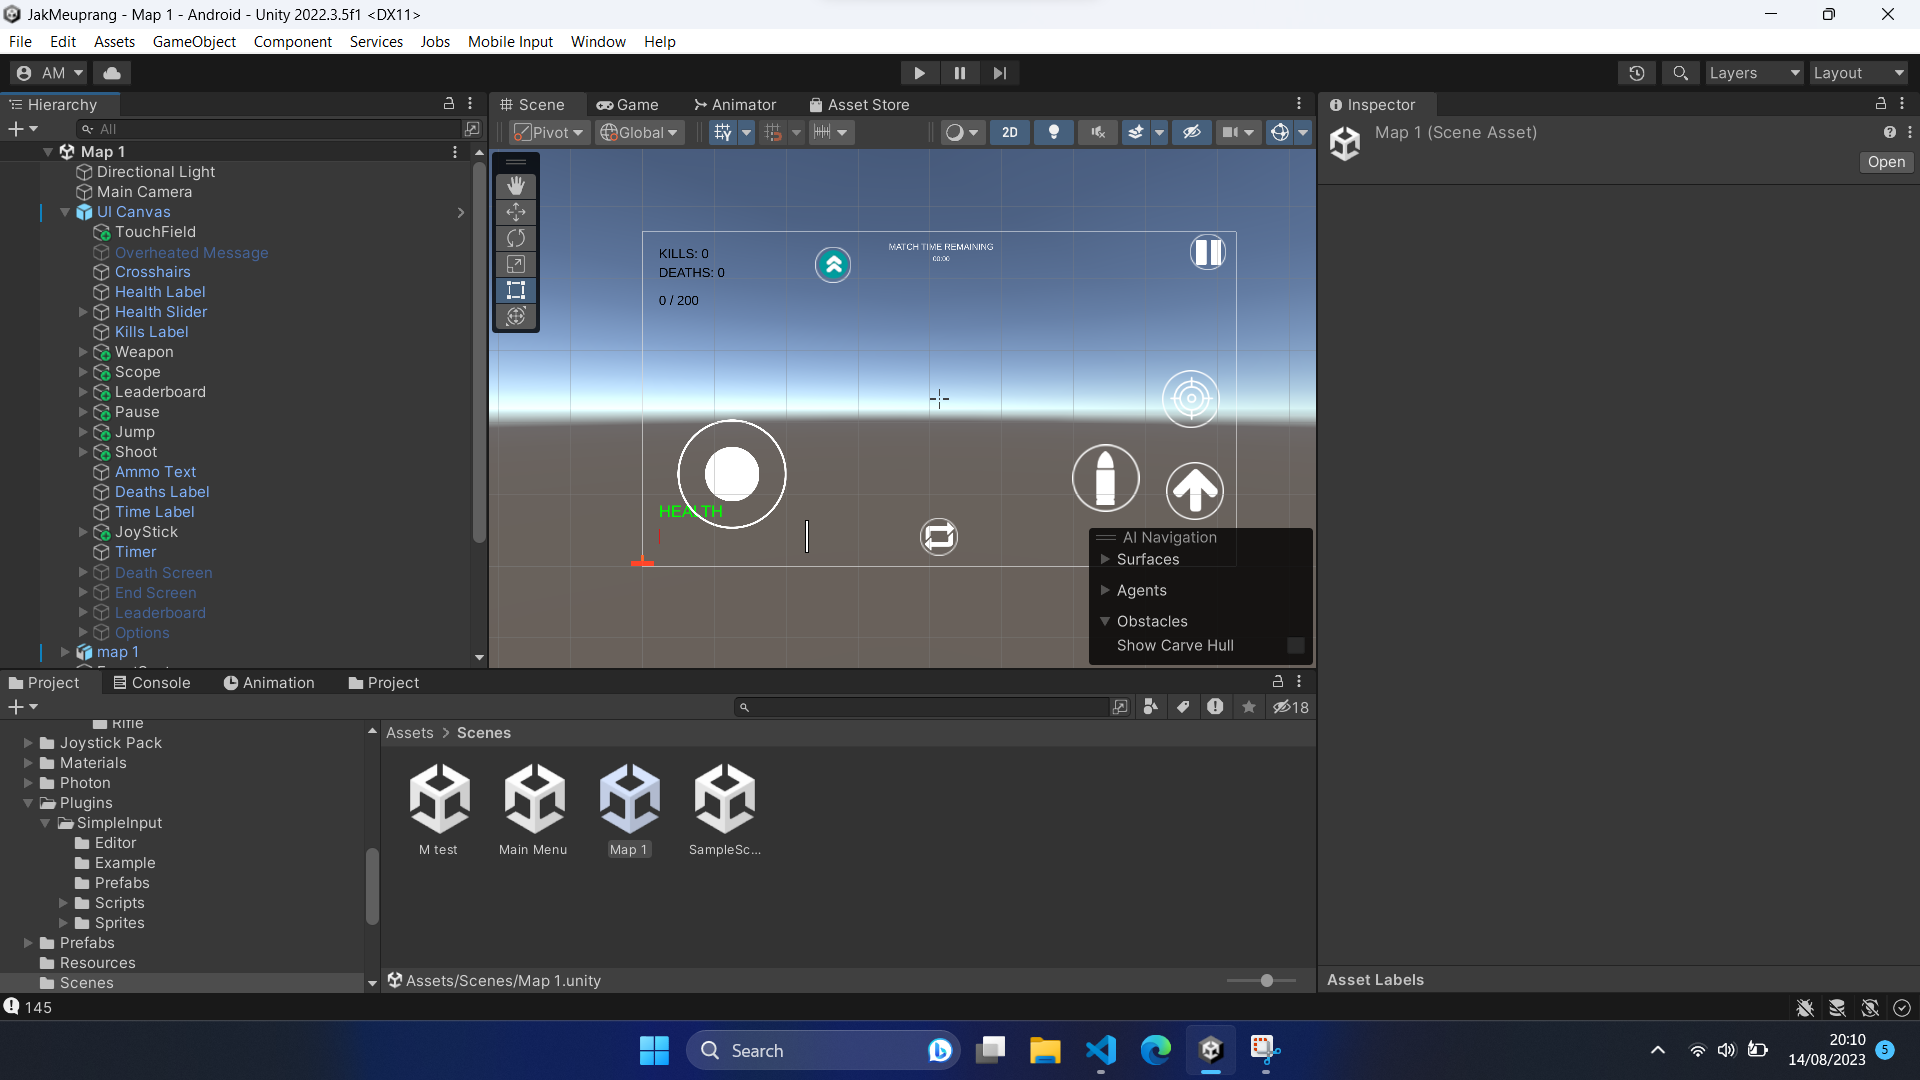
\includegraphics[width=10cm]{mobile-input.png}
        \caption{Tampilan Pembuatan \textit{Mobile Input}}
        \label{fig:mobileinput}
    \end{figure}
\item Pembuatan Map \\
Tahap ini adalah tahap pembuatan map yang digunakan saat bermain, map ini menggunakan asset low poly yang diberikan secara gratis dan dimplementasikan
\begin{figure}[h]
    \centering
    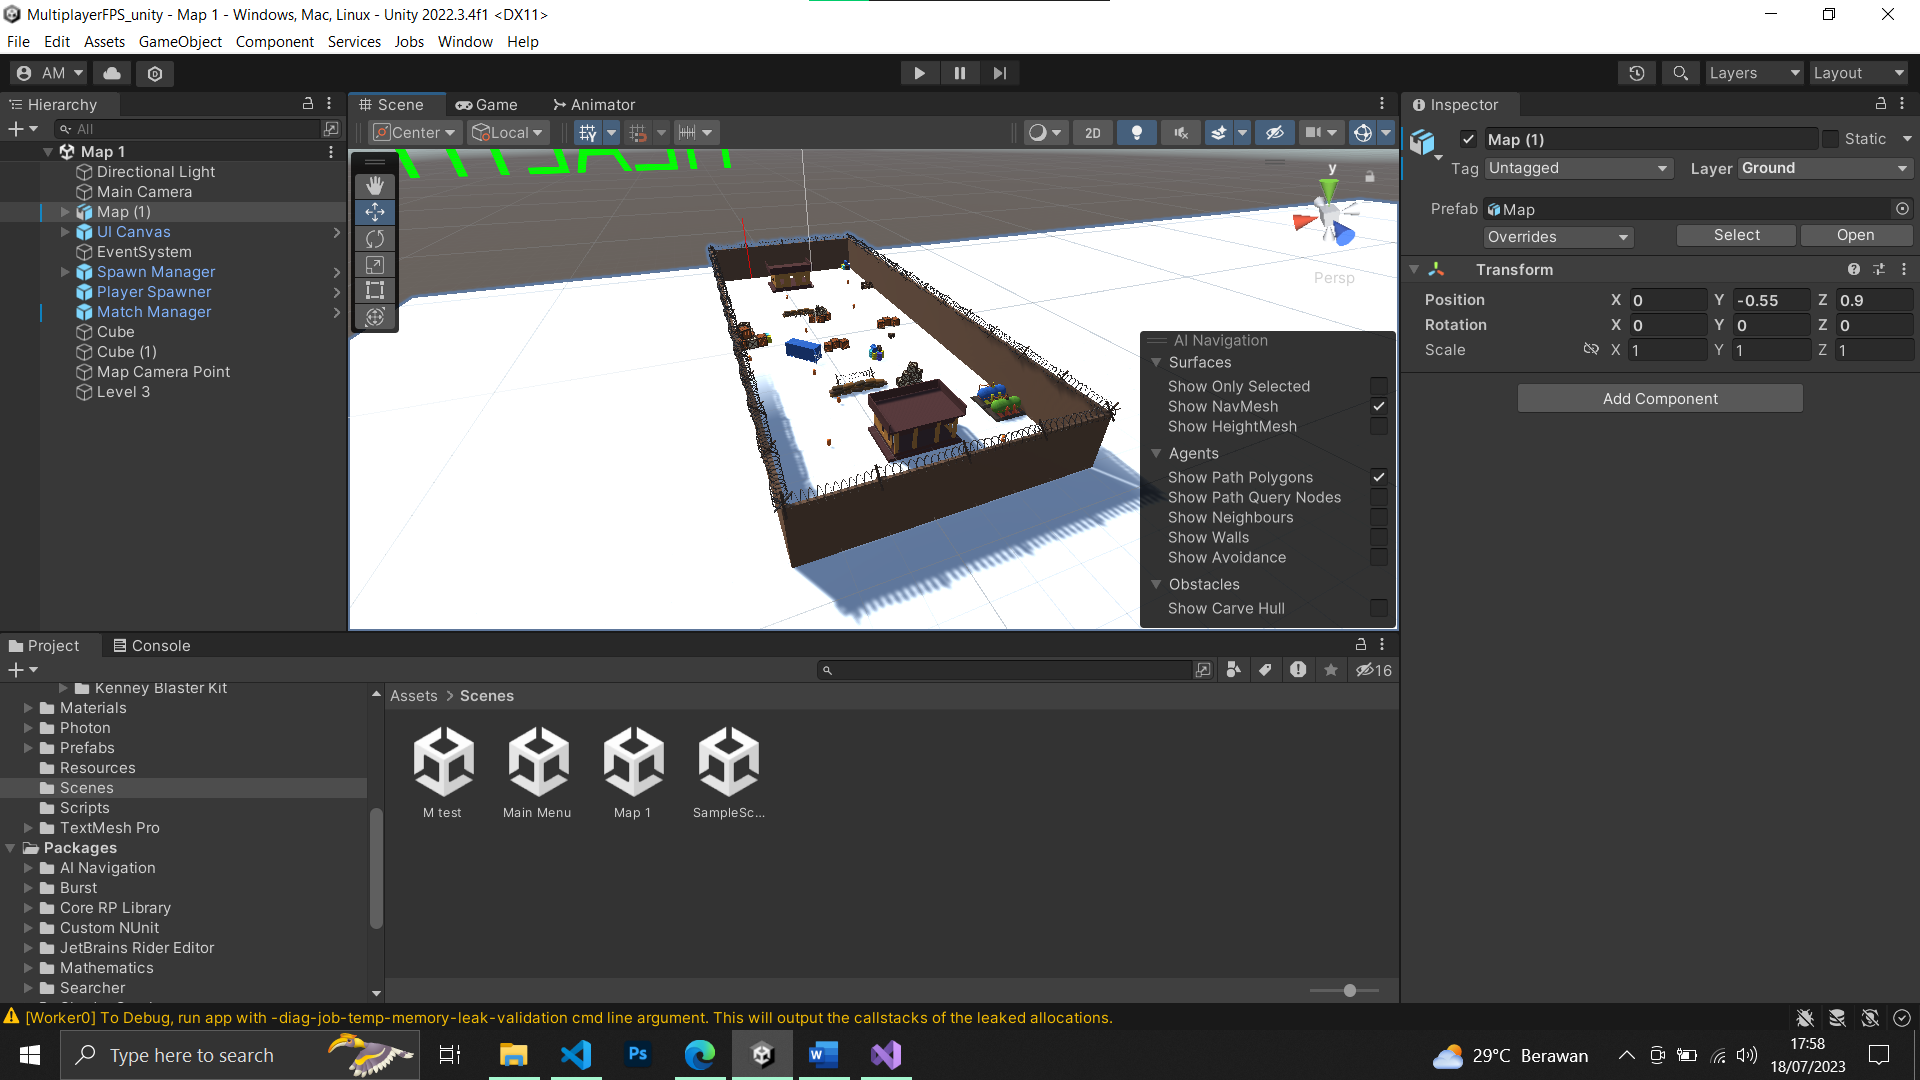
\includegraphics[width=10cm]{pembuatanmap.png}
    \caption{Tampilan Pembuatan Map}
    \label{fig:pembuatanmap}
\end{figure}
\newpage
\item Pembuatan Spawn Point \\ 
Pada tahap ini, memberikan beberapa titik spawn player secara random, jika player di\textit{kill} oleh player lain, maka sistem akan memberikan titik spawn yang sudah ditentukan.
\begin{figure}[h]
    \centering
    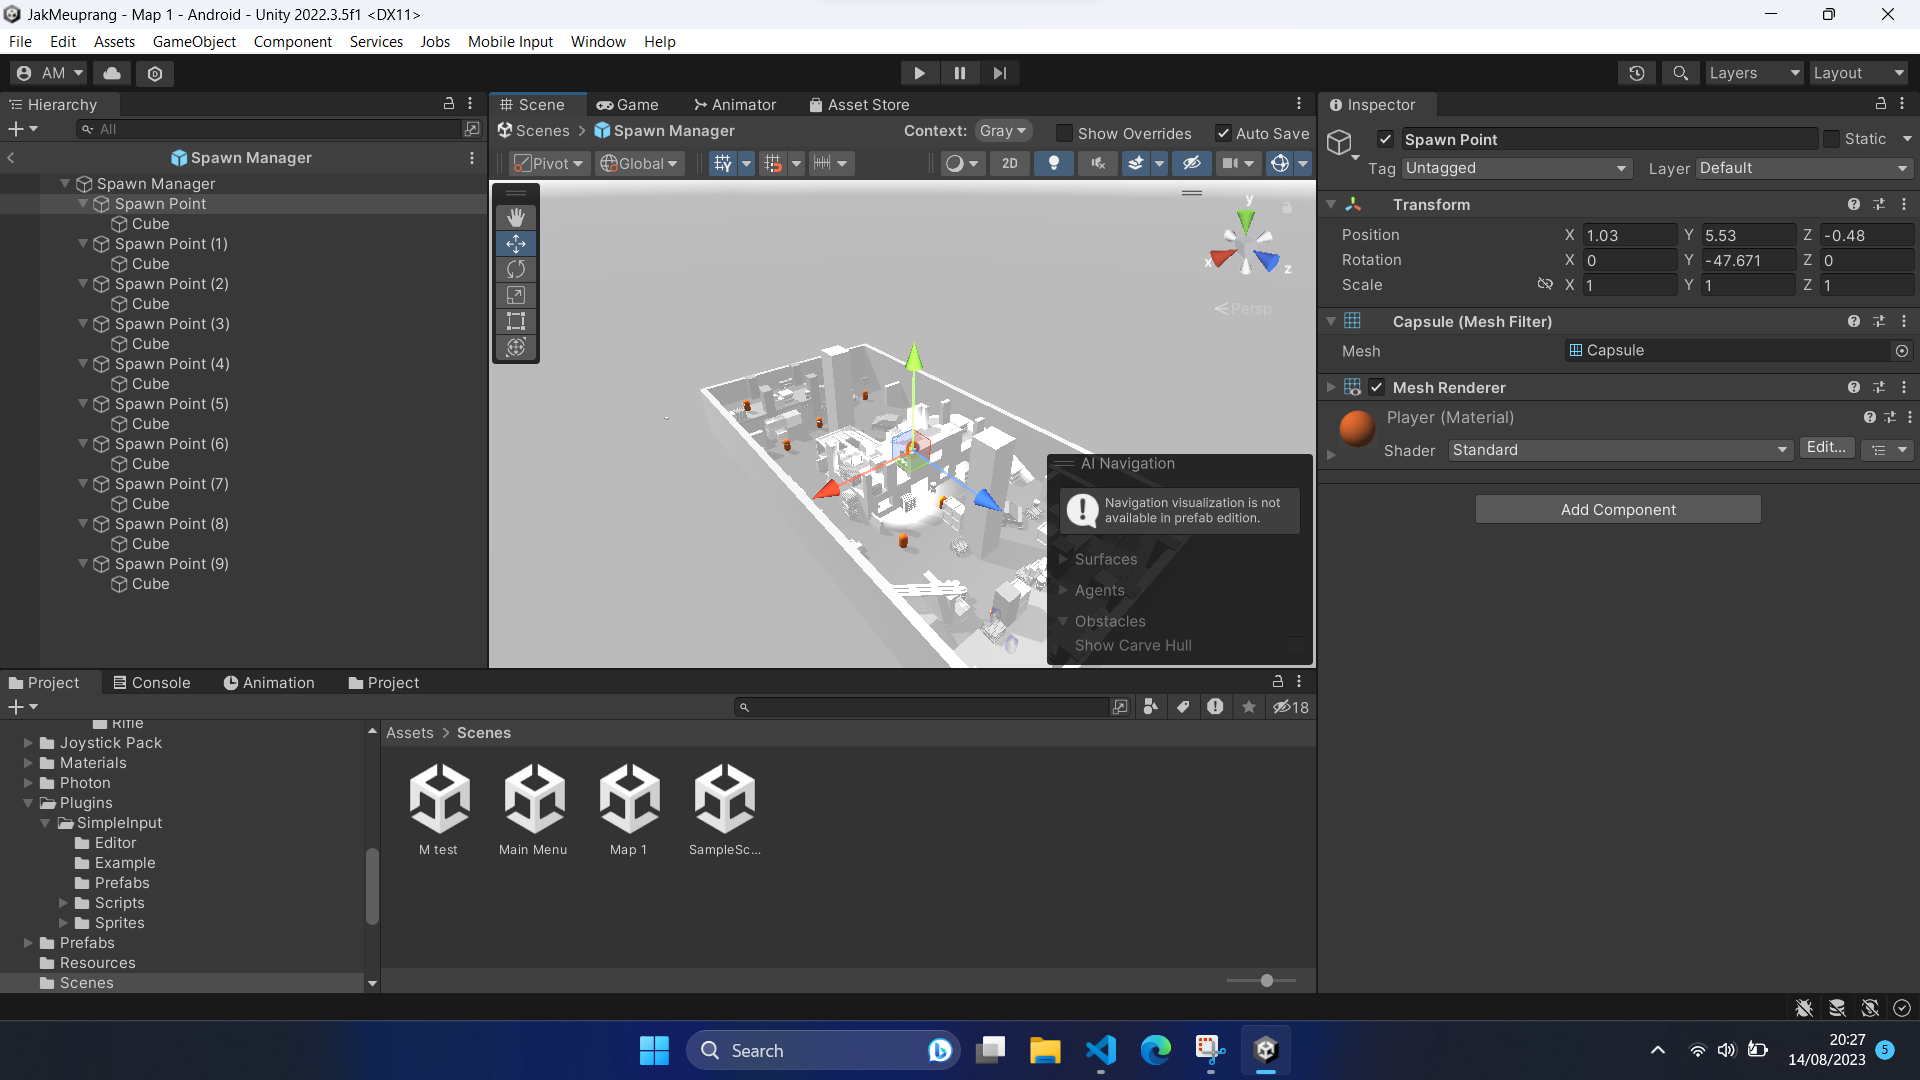
\includegraphics[width=10cm]{pembuatan-spawn.png}
    \caption{Tampilan Pembuatan Map}
    \label{fig:pembuatanspawn}
\end{figure}
\item Pembuatan Animasi Senjata \\
Tahap ini merupakan pembuatan animasi controller pada setiap setiap senjata yang ada yaitu pisau, m14, dan pistol.
\begin{figure}[h]
    \centering
    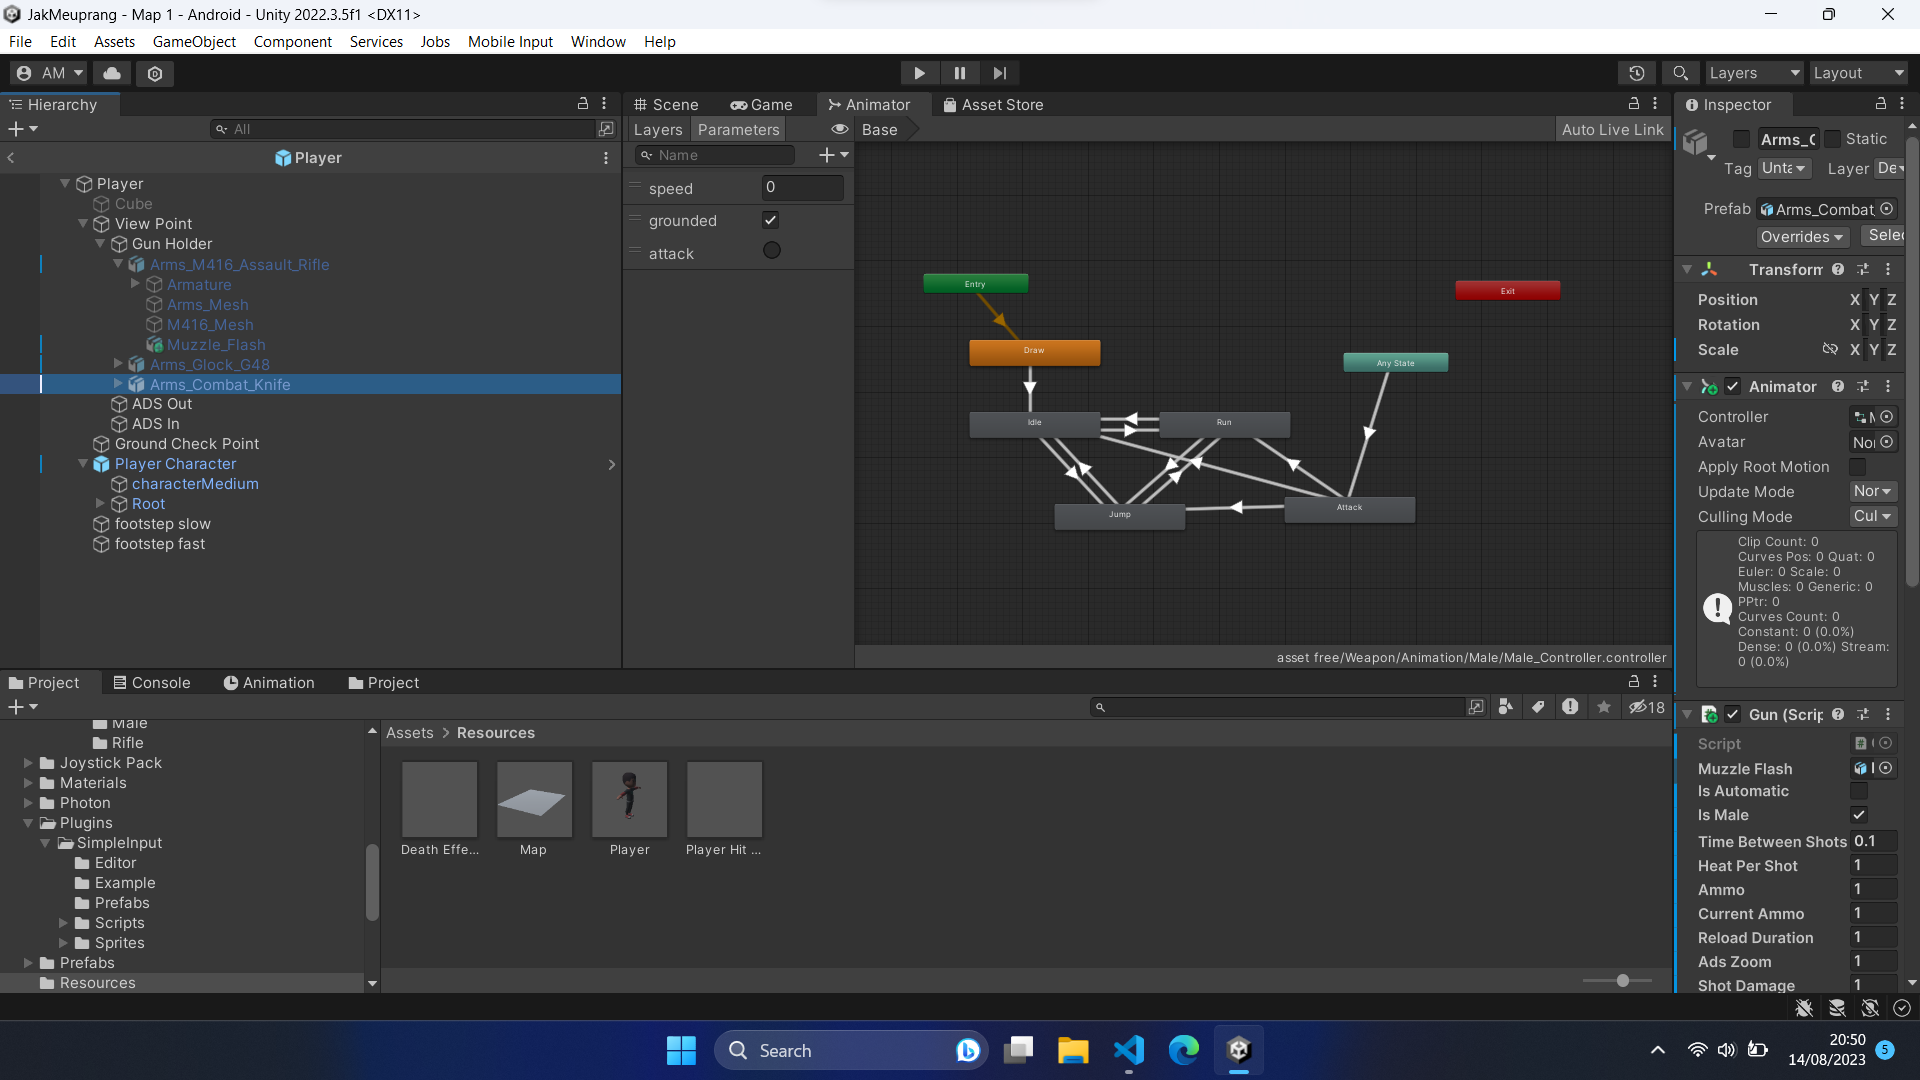
\includegraphics[width=10cm]{animasi-knife.png}
    \caption{Tampilan Pembuatan Animasi Knife}
    \label{fig:animasiknife}
\end{figure}
\newpage
\begin{figure}[h]
    \centering
    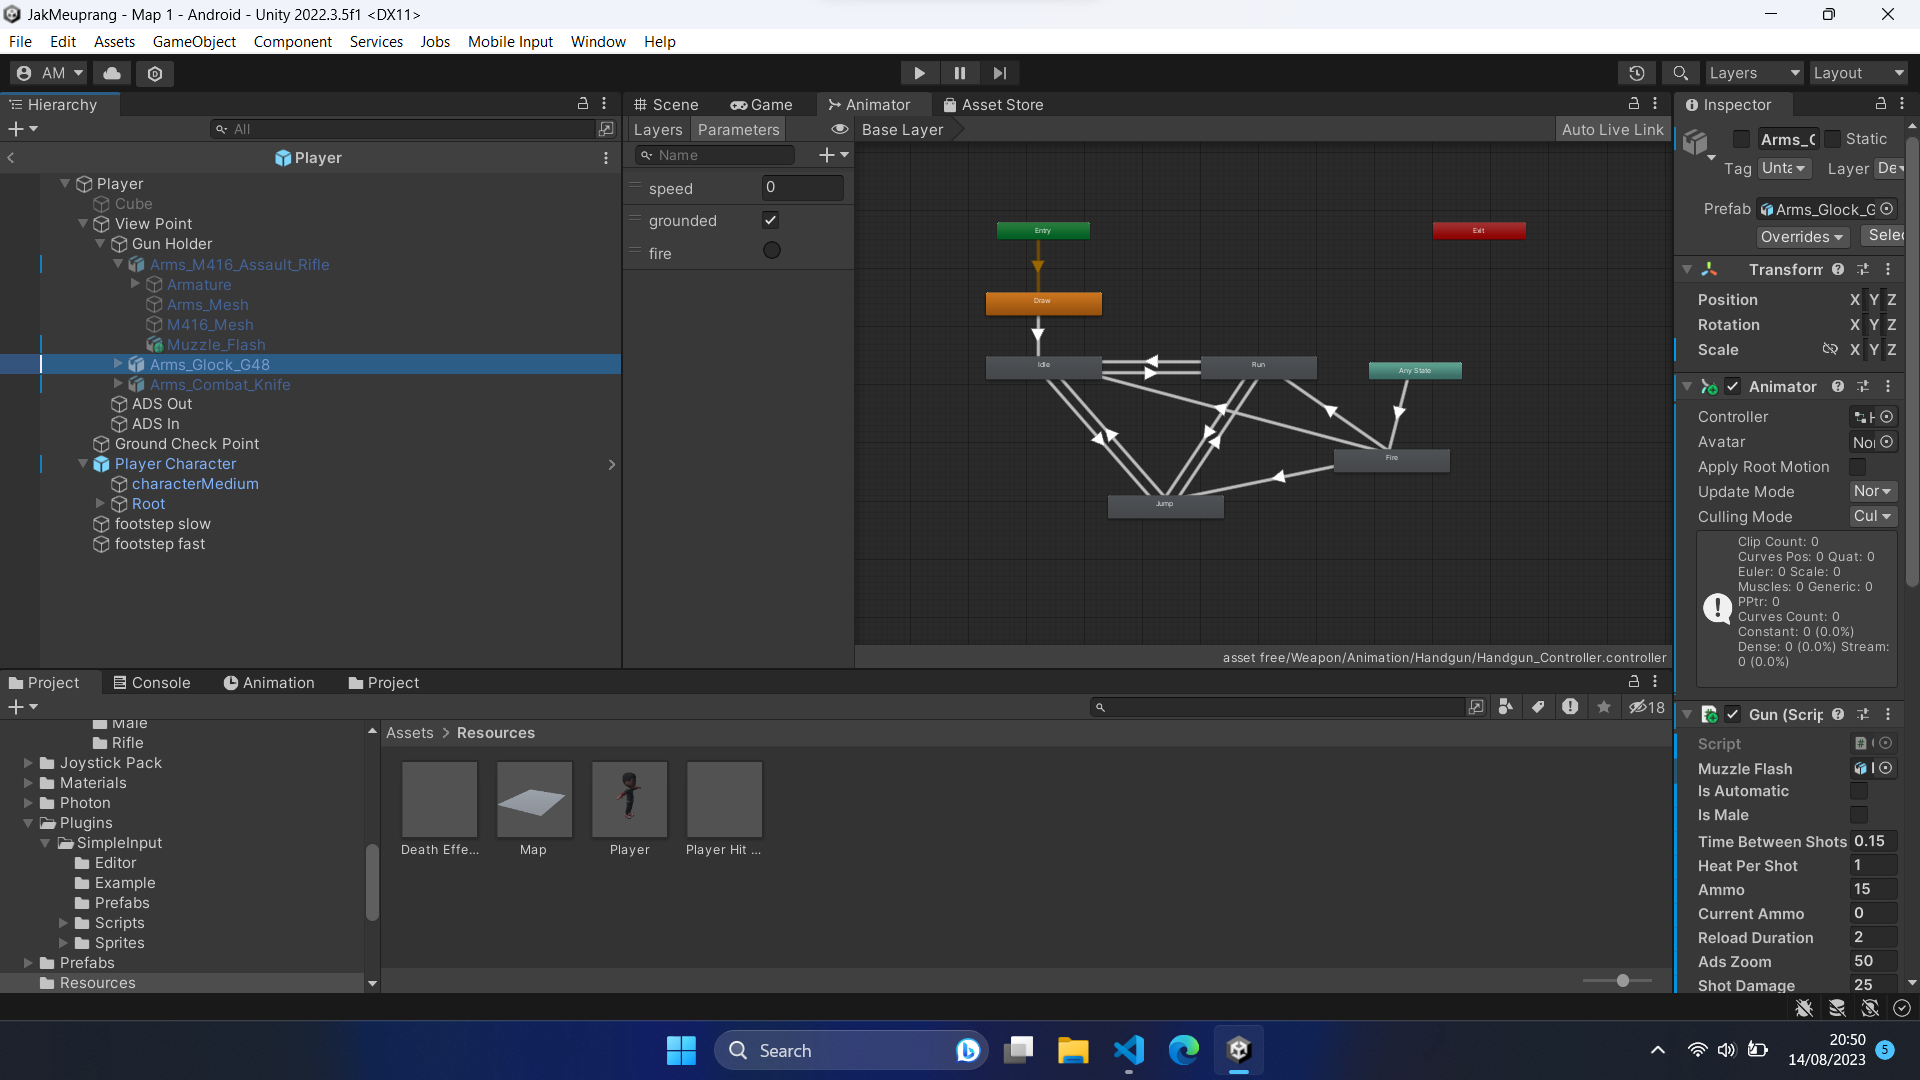
\includegraphics[width=10cm]{animasi-pistol.png}
    \caption{Tampilan Pembuatan Animasi Pistol}
    \label{fig:animasipistol}
\end{figure}
\begin{figure}[h]
    \centering
    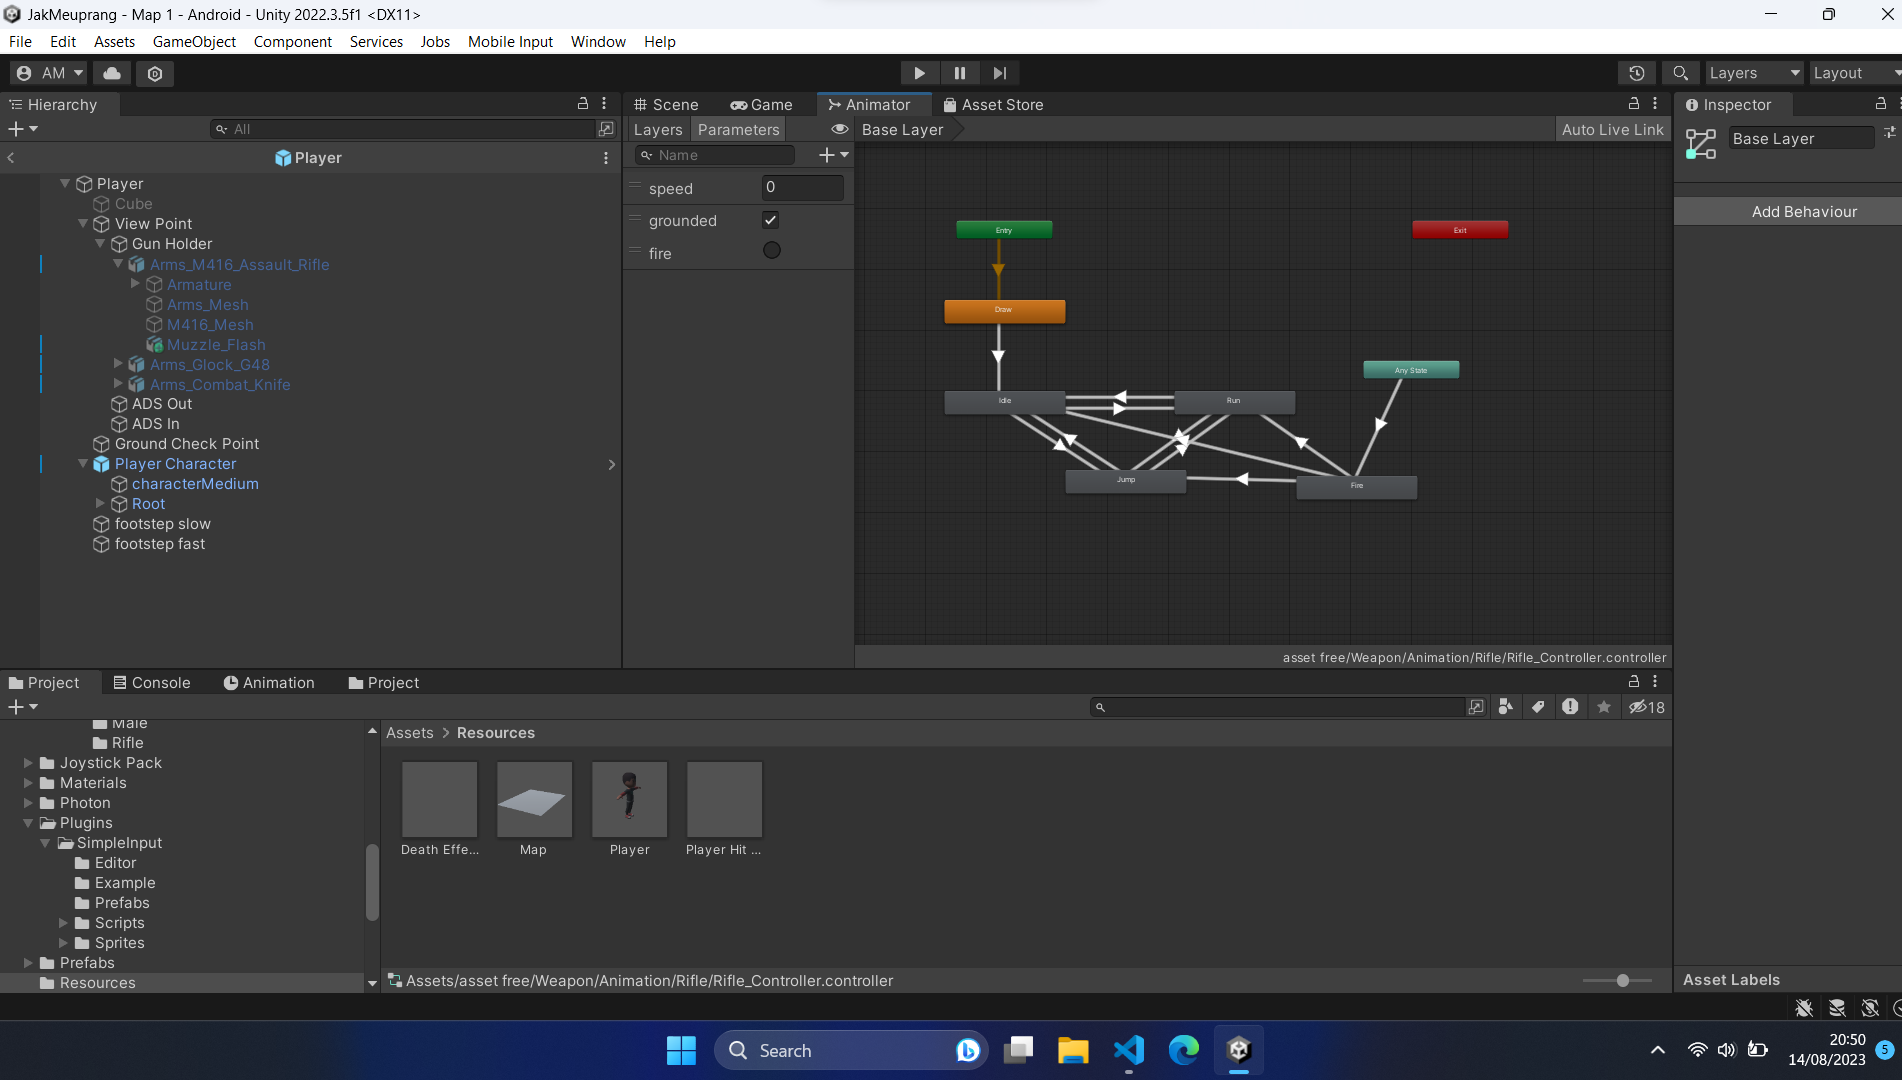
\includegraphics[width=10cm]{animasi-rifle.png}
    \caption{Tampilan Pembuatan Animasi Rifle}
    \label{fig:animasirifle}
\end{figure}
\end{enumerate}

% \newpage
% \subsection{Program}
% \noindent

% Pada bagian ini akan menampilkan source code yang akan menjalankan dari interaksi interkasi object object yang telah dibuat seperti berjalan, menembak, memasuki room dan lainnya.

% \begin{enumerate}
%     \item Implementasi Server Photon \\
%     Code ini berfungsi untuk melakukan connecting ke server photon, dengan menutup menu lainnya terlebih dahulu, jika server sudah terkoneksi maka akan masuk kedalam instance set nama dan menu.
%     \begin{figure}[h]
%         \centering
%         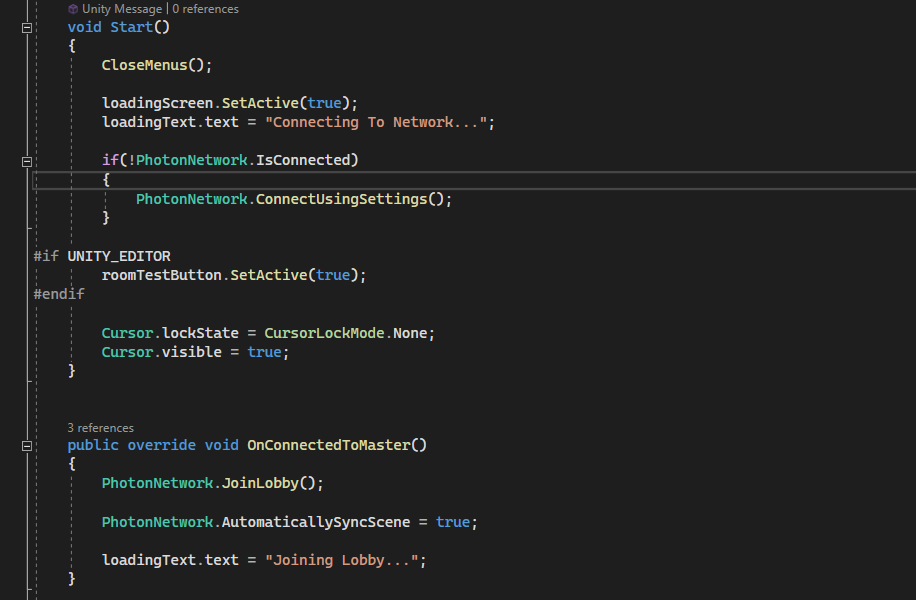
\includegraphics[width=10cm]{implementasiphoton.png}
%         \caption{Tampilan Code Photon}
%         \label{fig:connectingp}
%     \end{figure}
%     \item \textit{Source Code} Create Room \\
%     Pada code ini berfungsi untuk melakukan pembuatan room dengan memberikan nama room, max player, dan memanggil photonetwork untuk melakukan pembuatan room.
%     \newpage
%     \begin{figure}[h]
%         \centering
%         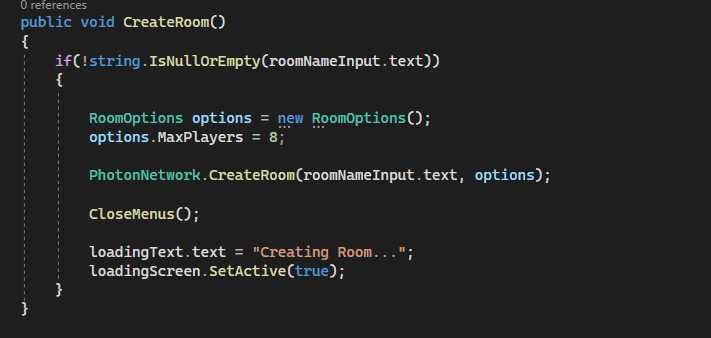
\includegraphics[width=10cm]{codepembuatanroom.png}
%         \caption{Tampilan Code Pembuatan Room}
%         \label{fig:pembuatanroom}
%     \end{figure}
%     \item \textit{Source Code Joinned Room} \\
%     Code ini berfungsi untuk memberikan instance jika player join room akan menampikan room yang dimasuk dengan player player yang tersedia pada room tersebut.
%     \begin{figure}[h]
%         \centering
%         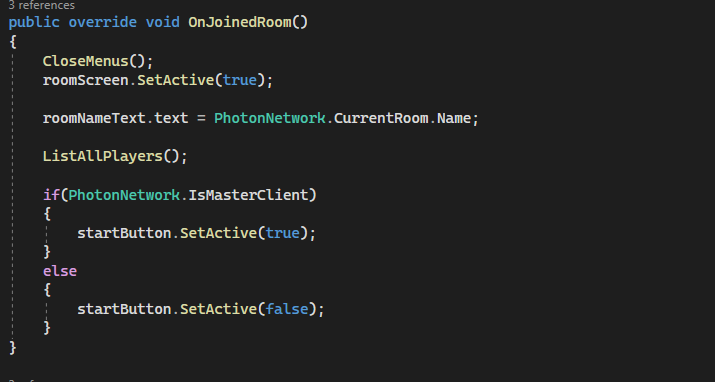
\includegraphics[width=10cm]{joinnedroom.png}
%         \caption{Tampilan Code Joinned Room}
%         \label{fig:joinnedroom}
%     \end{figure}
%     \item \textit{Source Code Start Game}\\
%     Code ini berfungsi untuk melakukan pemindahan instance ke scene map jika player memulai room yang telah dibuat.
%     \begin{figure}[h]
%         \centering
%         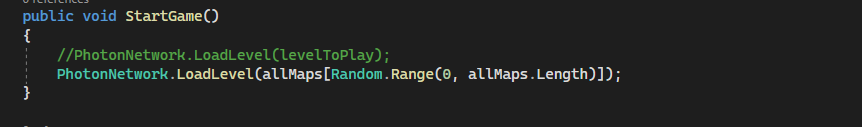
\includegraphics[width=10cm]{startgame.png}
%         \caption{Tampilan Code Start Game}
%         \label{fig:startgame}
%     \end{figure}
%     \newpage
%     \item \textit{Source Code Player Controller} \\
%     Code ini berfungsi untuk memberikan instance pertama player respawn saat dimainkan
%     \begin{figure}[h]
%         \centering
%         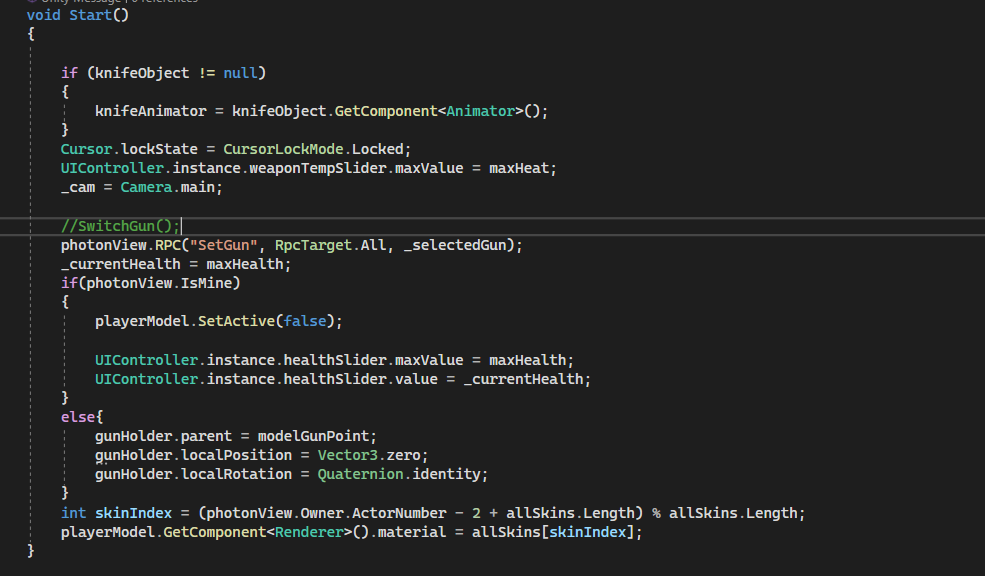
\includegraphics[width=10cm]{playerinstance.png}
%         \caption{Tampilan Code Player Instance}
%         \label{fig:playerinstance}
%     \end{figure}
%     \item \textit{Source Code Switch Gun} \\ 
%     Code ini berfungsi untuk melakukan pergantian senjata pada player.
%     \begin{figure}[h]
%         \centering
%         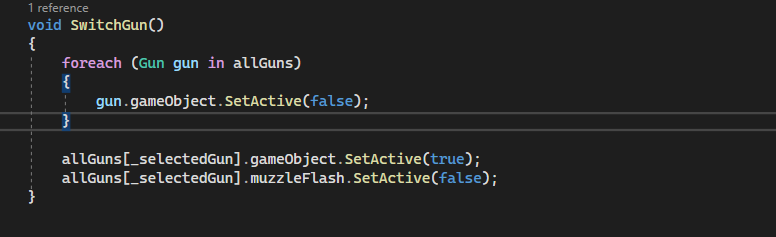
\includegraphics[width=10cm]{switchgun.png}
%         \caption{Tampilan Code Switch}
%         \label{fig:switchgun}
%     \end{figure}
%     \item \textit{Source Code Damage} \\
%     Code ini berfungsi menerima damage pada player.
%     \newpage
%     \begin{figure}[h]
%         \centering
%         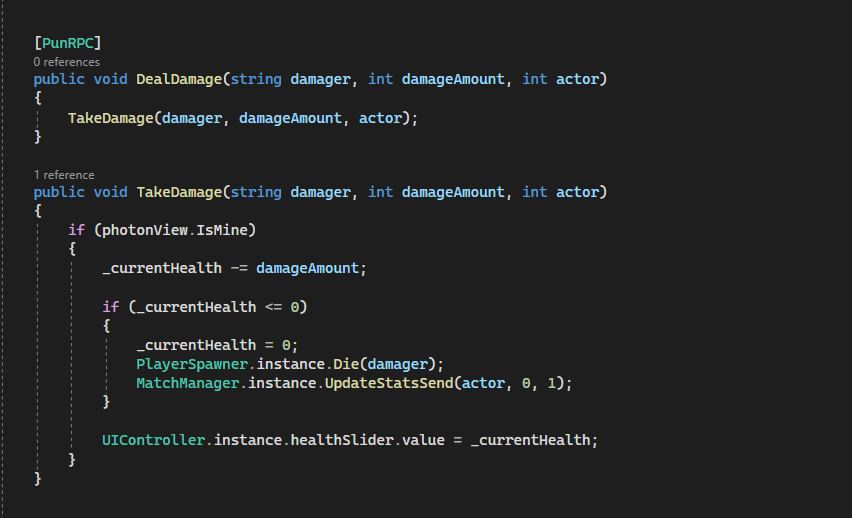
\includegraphics[width=10cm]{takedamage.png}
%         \caption{Tampilan Code Take Damage}
%         \label{fig:takedamage}
%     \end{figure}
%     \item \textit{Source Code Shoot} \\ 
%     Code ini berfungsi untuk membuat player tembakan.
%     \begin{figure}[h]
%         \centering
%         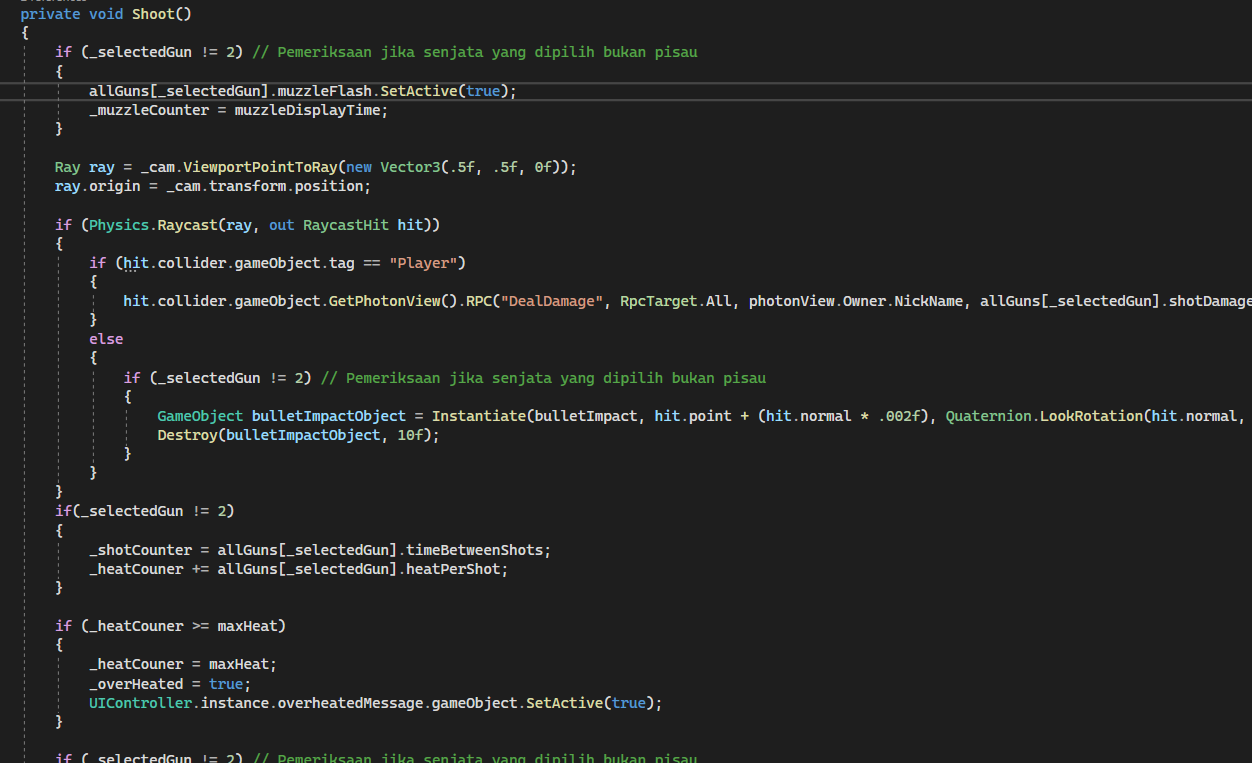
\includegraphics[width=10cm]{shoot.png}
%         \caption{Tampilan Code Shoot}
%         \label{fig:shoot}
%     \end{figure}
%     \newpage
%     \item \textit{Source Code Knife} \\ 
%     Code ini berfungsi untuk membuat player memberikan animasi \textit{Knife}.
%     \begin{figure}[h]
%         \centering
%         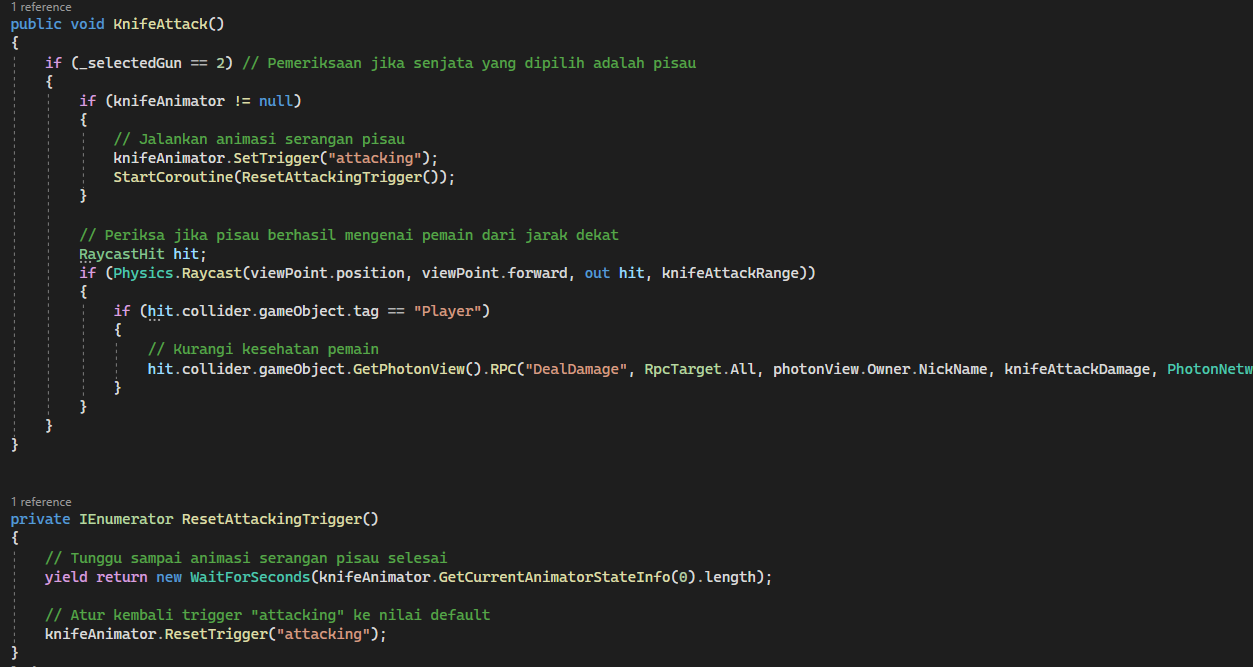
\includegraphics[width=10cm]{knife.png}
%         \caption{Tampilan Code Knife}
%         \label{fig:knife}
%     \end{figure}
%     \item \textit{Source Code Movement Player} \\ 
%     Code ini Berfungsi untuk membuat bergerakan player yang didapat dari inputan.
%     \begin{figure}[h]
%         \centering
%         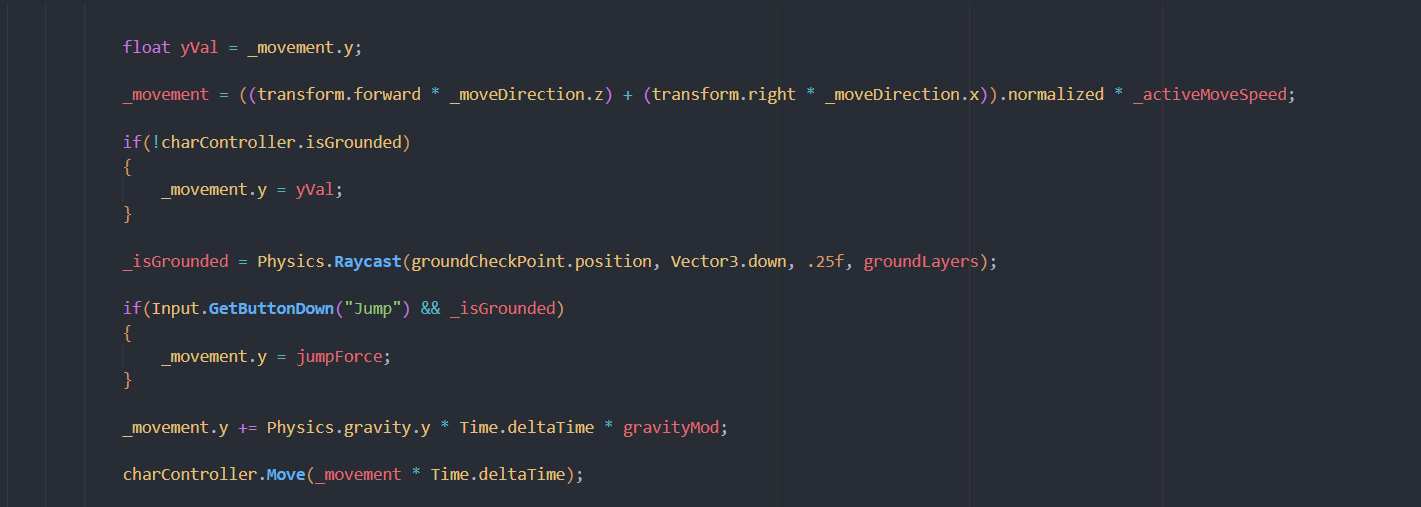
\includegraphics[width=10cm]{player-movement.png}
%         \caption{Tampilan Code Player Movement}
%         \label{fig:movementp}
%     \end{figure}
%     \item \textit{Source Code Match Manager} \\
%     Code ini berfungsi untuk melakukan instance match manager untuk mengatur logika selama bermain.
%     \newpage
%     \begin{figure}[h]
%         \centering
%         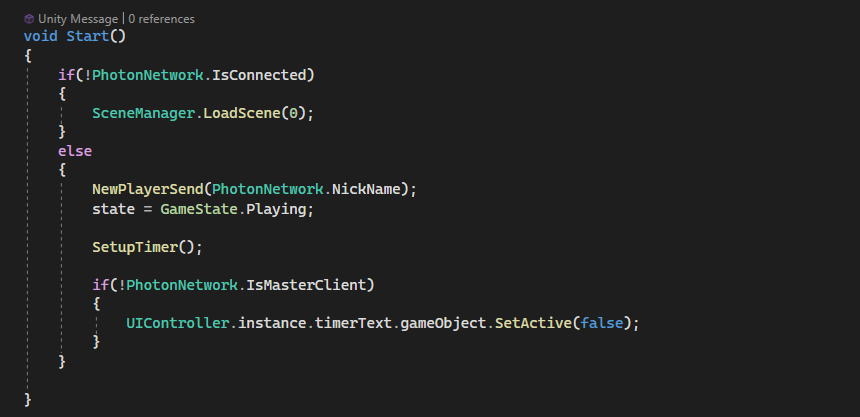
\includegraphics[width=10cm]{matchmanager.png}
%         \caption{Tampilan Code Match Manger}
%         \label{fig:matchmanager}
%     \end{figure}
%     \item \textit{Source Code Leaderboard} \\ 
%     Code ini berfungsi untuk menampilkan leaderboard saat bermain.
%     \begin{figure}[h]
%         \centering
%         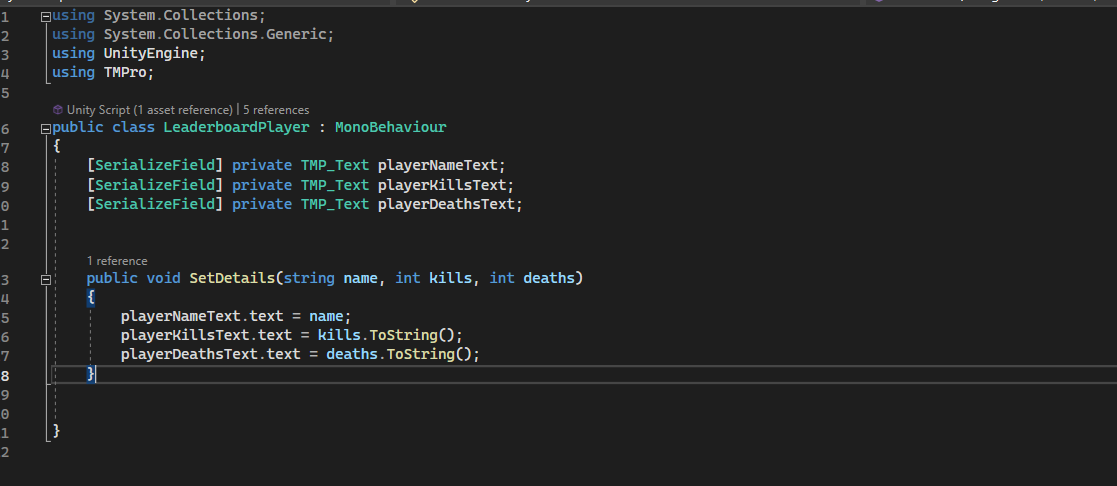
\includegraphics[width=10cm]{leaderboard.png}
%         \caption{Tampilan Code LeaderBoard}
%         \label{fig:leaderboard}
%     \end{figure}
%     \item \textit{Source Code Spawn Manager}\\
%     Code ini berfungsi untuk memberikan spawn player secara random dengan titik yang telah ditentukan.
%    \newpage
%     \begin{figure}[h]
%         \centering
%         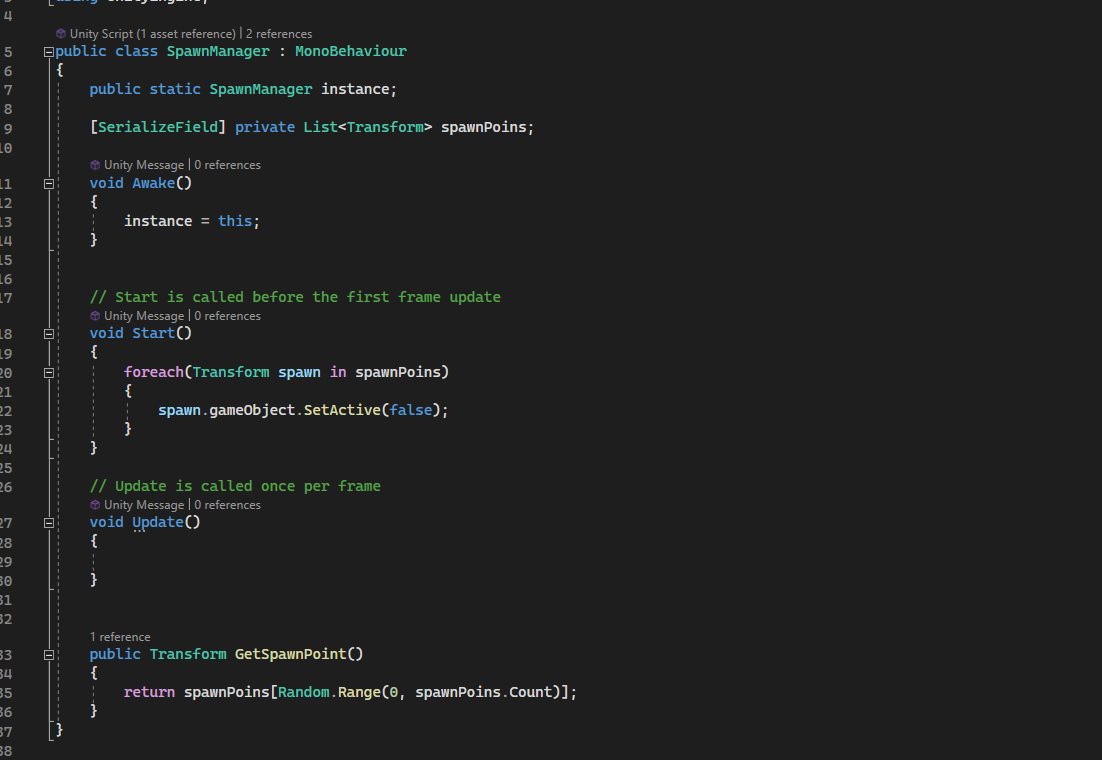
\includegraphics[width=10cm]{spawnmanager.png}
%         \caption{Tampilan Code Spawn Manager}
%         \label{fig:spawnmanager}
%     \end{figure}
%     \item \textit{Source Code Player Spawner} \\ 
%     Code ini berfungsi untuk melakukan instance spawn dan matinya player.
%     \begin{figure}[h]
%         \centering
%         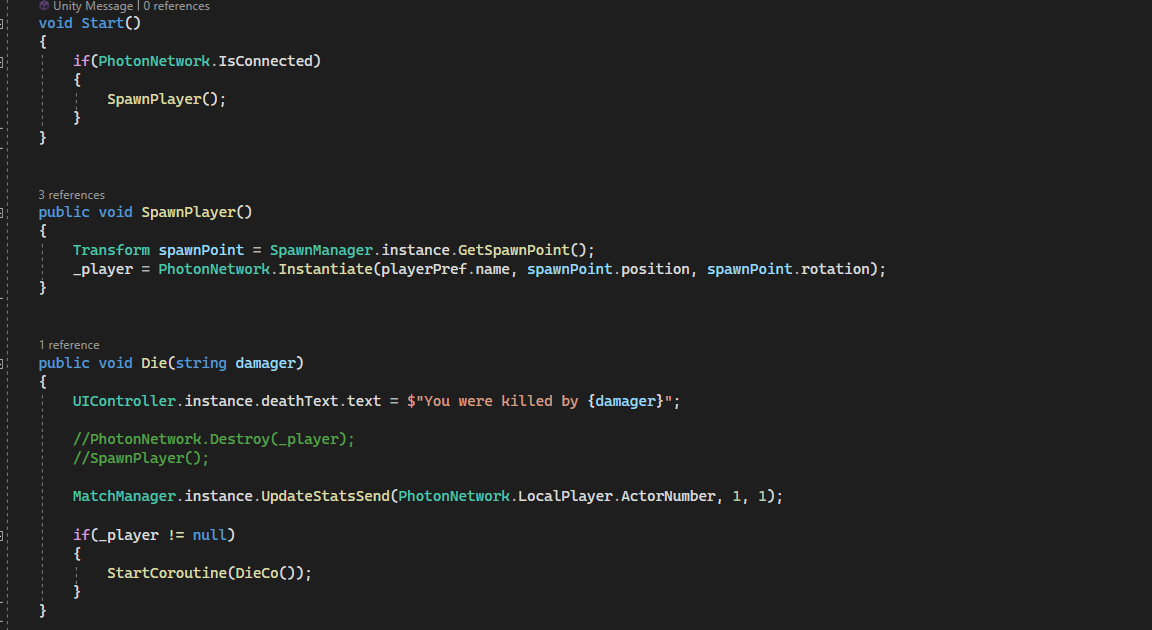
\includegraphics[width=10cm]{playerspawner.png}
%         \caption{Tampilan Code Player Spawner}
%         \label{fig:playerspawner}
%     \end{figure}
%     \item \textit{Source Code Gun} \\ 
%     Code ini berfungsi untuk memberikan algoritma pada senajata yang digunakan.
%     \newpage
%     \begin{figure}[h]
%         \centering
%         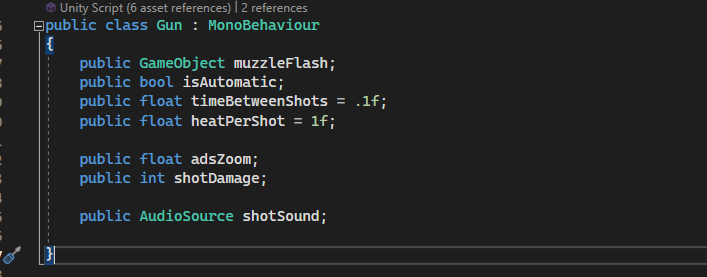
\includegraphics[width=10cm]{gun.png}
%         \caption{Tampilan Code Gun}
%         \label{fig:gun}
%     \end{figure}
% \end{enumerate}

\section{Pengujian Game}
\noindent

Pada tahap ini, peneliti melakukan pengujian yaitu berupa pengujain sistem, grafis, interface, sinkronisasi dan pengujian jaringan.

\subsection{Uji Coba Pengguna}
\noindent

Dilakukan pengujian terhadap pengguna untuk 
memberikan timbal balik akurasi penilaian untuk pengujian 
performa. Berikut Daftar nama penguji pada uji coba pengguna 
yang dapat dilihat pada tabel \ref{tab:pengguna-uji}.
\newpage

\begin{table}[h]
    \centering
    \caption{Daftar Pengguna Uji Coba}
    \label{tab:pengguna-uji}
    \begin{tabular}{|l|l|l|}
    \hline
    \textbf{No} & \textbf{Nama}          & \textbf{Keterangan Device} \\ \hline
    1           & Ahlul Mukhramin        & Redmi Note 8               \\ \hline
    2           & Aldi Ferdian           & Realme 7                   \\ \hline
    3           & Rizki Ramadhan         & Samsung                    \\ \hline
    4           & Muhammad Rizki Afrizal & Redmi Note 7               \\ \hline
    5           & Mujibullah             & Vivo y15                   \\ \hline
    \end{tabular}
    \end{table}

Berikut hasil penilaian pengguna terhadap Kelancaran permainan, dan Kesesuaian GUI Pada tabel \ref{tab:pengujian-hasil}.

\begin{table}[h]
    \centering
    \caption{Hasil Pengujian Pengguna}
    \label{tab:pengujian-hasil}
    \begin{tabular}{|lllllll|l|}
    \hline
    \multicolumn{1}{|l|}{}                              & \multicolumn{1}{c|}{}                                                & \multicolumn{5}{c|}{\textbf{Penilaian}}                                                                                                                                 &                                      \\ \cline{3-7}
    \multicolumn{1}{|l|}{\multirow{-2}{*}{\textbf{No}}} & \multicolumn{1}{c|}{\multirow{-2}{*}{\textbf{Keterangan Pengujian}}} & \multicolumn{1}{c|}{\textbf{1}} & \multicolumn{1}{c|}{\textbf{2}} & \multicolumn{1}{c|}{\textbf{3}} & \multicolumn{1}{c|}{\textbf{4}} & \multicolumn{1}{c|}{\textbf{5}} & \multirow{-2}{*}{\textbf{Rata Rata}} \\ \hline
    \multicolumn{1}{|l|}{1}                             & \multicolumn{1}{l|}{Kelancaran FPS Permainan}                        & \multicolumn{1}{l|}{0}          & \multicolumn{1}{l|}{0}          & \multicolumn{1}{r|}{0}          & \multicolumn{1}{l|}{0}          & 5                               & 100\%                                \\ \hline
    \rowcolor[HTML]{9B9B9B} 
    \multicolumn{2}{|l|}{\cellcolor[HTML]{9B9B9B}}                                                                             & \multicolumn{2}{l|}{\cellcolor[HTML]{9B9B9B}Sesuai}               & \multicolumn{3}{l|}{\cellcolor[HTML]{9B9B9B}Tidak}                                                  &                                      \\ \hline
    \multicolumn{1}{|l|}{2}                             & \multicolumn{1}{l|}{Kesesuaian GUI Dengan Device}                    & \multicolumn{2}{l|}{5}                                            & \multicolumn{3}{l|}{0}                                                                              & 100\%                                \\ \hline
    \multicolumn{7}{|c|}{Total Rata Rata}                                                                                                                                                                                                                                                                & 100\%                                \\ \hline
    \end{tabular}
    \end{table}

\subsection{Pengujian Grafis 3D}
\noindent

Uji ini berupa perhitungan kecepatan \textit{frame} per detik pada perangkat Android dalam me-render objeck 3D. Sebuah permainan video akan terasa lancar pada standar \textit{framerate} 24. Pengujian ini berlangsung menggunnakan permainan itu sendiri. Hasilnya dapat dilihat pada tabel \ref{tb:tabel-grafis}.

\begin{table}[h]
    \centering
    \caption{Hasil Pengujian Grafis 3D}
    \label{tb:tabel-grafis}
    \begin{tabular}{|l|l|l|l|}
    \hline
    \multicolumn{1}{|c|}{Nama Perangkat} & \multicolumn{1}{c|}{\begin{tabular}[c]{@{}c@{}}Fps\\ Minimum\end{tabular}} & \multicolumn{1}{c|}{\begin{tabular}[c]{@{}c@{}}Fps\\ Maksimum\end{tabular}} & \multicolumn{1}{c|}{\begin{tabular}[c]{@{}c@{}}Fps\\ Rata-Rata\end{tabular}} \\ \hline
    Redmi Note 8   & 27  & 35 & 30 \\ \hline
    Vivo y15       & 29  & 30 & 29 \\ \hline
    Redmi Note 7   & 29  & 37 & 35 \\ \hline
    Realme 7    & 29  & 60 & 54 \\ \hline
    Samsung    & 30  & 60 & 45 \\ \hline
    \multicolumn{3}{|c|}{Total rata-rata} & 34.6 \\ \hline
    \multicolumn{3}{|l|}{Presentase Terhadap Standar Kelancaran (24FPS)} & 100\%  \\ \hline
    \end{tabular}
    \end{table}
\newpage
\subsection{Uji Interface GUI}
\noindent

Uji coba ini berupa pengecekan kompabilty GUI di layar \textit{landscape orientatio} pada perangkat yang berbeda-beda dan 
mengacu terhadap pengujian pengguna dengan device yang 
dimiliki. Hasilnya dapat dilihat pada Tabel \ref{tb:tabel-interface}

\begin{table}[h]
    \centering
    \caption{Hasil Pengujian Interface}
    \label{tb:tabel-interface}
    \begin{tabular}{|c|c|}
    \hline
    Nama Perangkat & \begin{tabular}[c]{@{}c@{}}Kesesuaian\\ GUI Pada Layar\end{tabular} \\ \hline
    Redmi Note 8   & Sesuai                                                              \\ \hline
    Vivo y15       & Sesuai                                                              \\ \hline
    Redmi Note 7   & Sesuai                                                              \\ \hline
    Poco x3 Pro    & Sesuai                                                              \\ \hline
    Rog Phone 2    & Sesuai                                                              \\ \hline
    \end{tabular}
    \end{table}
\newpage
% \subsection{Pengujian Blackbox Testing}
% \noindent

% Pengujian blackbox untuk menguji fungsi sistem atau kekurangan pada 
% perangkat lunak yang diuji agar menjadi lebih baik dan dapat diminimalisir 
% terjadinya kekurangan pada sistem
% \begin{enumerate}
%     \item Tombol Cari Room \\
% \begin{table}[h]
%     \centering
%     \caption{Hasil Pengujian Cari Room}
%     \label{tb:tabel-cariroom}
%     \begin{tblr}{
%       vlines,
%       hline{1,7} = {-}{0.08em},
%       hline{2} = {-}{},
%       hline{3-6} = {4,6}{},
%     }
%     ID  & {Rincian \\Pengujian} & {Hasil yang\\di harapkan}             & Player & {Hasil yang \\didapatkan}             & Keterangan \\
%     R01 & {Tombol \\Cari Room}  & {Menampilkan \\Panel\\Pencarian Room} & 1      & {Menampilkan \\Panel\\Pencarian Room} & Berhasil   \\
%         &                       &                                       & 2      &                                       & Berhasil   \\
%         &                       &                                       & 3      &                                       & Berhasil   \\
%         &                       &                                       & 4      &                                       & Berhasil   \\
%         &                       &                                       & 5      &                                       & Berhasil   
%     \end{tblr}
%     \end{table}
%     \newpage
%     \item Tombol Buat Room \\
%     \begin{table}[h]
%         \centering
%         \caption{Hasil Pengujian Buat Room}
%         \label{tb:tabel-buatroom}
%         \begin{tblr}{
%           vlines,
%           hline{1,7} = {-}{0.08em},
%           hline{2} = {-}{},
%           hline{3-6} = {4,6}{},
%         }
%         ID  & {Rincian \\Pengujian} & {Hasil yang\\di harapkan}                & Player & {Hasil yang \\didapatkan}               & Keterangan \\
%         B01 & {Tombol\\Buat Room}   & {Menampilkan \\Panel Inputan\\Nama Room} & 1      & {Menampilkan\\Panel Inputan\\Nama Room} & Berhasil   \\
%             &                       &                                          & 2      &                                         & Berhasil   \\
%             &                       &                                          & 3      &                                         & Berhasil   \\
%             &                       &                                          & 4      &                                         & Berhasil   \\
%             &                       &                                          & 5      &                                         & Berhasil   
%         \end{tblr}
%         \end{table}
%         \newpage
%         \item Tombol Exit Room \\
%         \begin{table}[h]
%             \centering
%             \caption{Hasil Pengujian Exit Room}
%         \label{tb:tabel-exitroom}
%             \begin{tblr}{
%               vlines,
%               hline{1,7} = {-}{0.08em},
%               hline{2} = {-}{},
%               hline{3-6} = {4,6}{},
%             }
%             ID  & {Rincian \\Pengujian} & {Hasil yang\\di harapkan}  & Player & {Hasil yang \\didapatkan} & Keterangan \\
%             E01 & {Tombol\\Exit Room}   & {Menampilkan~\\Menu Utama} & 1      & {Menampilkan\\Menu utama} & Berhasil   \\
%                 &                       &                            & 2      &                           & Berhasil   \\
%                 &                       &                            & 3      &                           & Berhasil   \\
%                 &                       &                            & 4      &                           & Berhasil   \\
%                 &                       &                            & 5      &                           & Berhasil   
%             \end{tblr}
%             \end{table}
%         \item Tombol About Game \\
%         \begin{table}[h]
%             \centering
%             \caption{Hasil Pengujian About Game}
%             \label{tb:tabel-aboutgame}
%             \begin{tblr}{
%               vlines,
%               hline{1,7} = {-}{0.08em},
%               hline{2} = {-}{},
%               hline{3-6} = {4,6}{},
%             }
%             ID  & {Rincian \\Pengujian} & {Hasil yang\\di harapkan} & Player & {Hasil yang \\didapatkan} & Keterangan \\
%             A01 & {Tombol\\About\\Game} & {Menampilkan\\Informasi}  & 1      & {Menampilkan\\Informasi}  & Berhasil   \\
%                 &                       &                           & 2      &                           & Berhasil   \\
%                 &                       &                           & 3      &                           & Berhasil   \\
%                 &                       &                           & 4      &                           & Berhasil   \\
%                 &                       &                           & 5      &                           & Berhasil   
%             \end{tblr}
%             \end{table}
%         \newpage
%         \item Tombol Keluar \\
%         \begin{table}[h]
%             \centering
%             \caption{Hasil Pengujian Keluar Game}
%             \label{tb:tabel-keluargame}
%             \begin{tblr}{
%               vlines,
%               hline{1,7} = {-}{0.08em},
%               hline{2} = {-}{},
%               hline{3-6} = {4,6}{},
%             }
%             ID  & {Rincian \\Pengujian} & {Hasil yang\\di harapkan} & Player & {Hasil yang \\didapatkan} & Keterangan \\
%             K01 & {Tombol\\Keluar}      & {Mengeluarkan\\Permainan} & 1      & {Mengeluarkan\\Permainan} & Berhasil   \\
%                 &                       &                           & 2      &                           & Berhasil   \\
%                 &                       &                           & 3      &                           & Berhasil   \\
%                 &                       &                           & 4      &                           & Berhasil   \\
%                 &                       &                           & 5      &                           & Berhasil   
%             \end{tblr}
%             \end{table}
% \end{enumerate}

% Pada Tabel \ref{tb:tabel-blackbox} untuk menampilkan menghitung persentase kelayakan menu game dari 5 pengguna.
% \begin{table}[h]
%     \centering
%     \caption{Hasil Pengujian Black Box}
%     \label{tb:tabel-blackbox}
%     \begin{tabular}{|ll|l|l|l|} 
%     \toprule
%     \multicolumn{1}{|l|}{\begin{tabular}[c]{@{}l@{}}Test\\Case\\Id\end{tabular}} & Penggunaan Berhasil                      & \begin{tabular}[c]{@{}l@{}}Pengunaan\\Tidak\\Berhasil\end{tabular} & Presentase & Hasil                 \\ 
%     \hline
%     R01                                                                          & 5                                        & 0                                                                  & $5/5 \times 100\%$  & 100\%                      \\ 
%     \hline
%     B01                                                                          & 5                                        & 0                                                                  & $5/5 \times 100\%$  & 100\%                      \\ 
%     \hline
%     E01                                                                          & 5                                        & 0                                                                  & $5/5 \times 100\%$  & 100\%                      \\ 
%     \hline
%     A01                                                                          & 5                                        & 0                                                                  & $5/5 \times 100\%$  & 100\%                      \\ 
%     \hline
%     K01                                                                          & 5                                        & 0                                                                  & $5/5 \times 100\%$  & 100\%                      \\ 
%     \hline
%                                                                                  & \multicolumn{1}{l}{Rata Rata Presentase} & \multicolumn{1}{l}{}                                               &            & 100\%  \\
%     \bottomrule
%     \end{tabular}
%     \end{table}

%     Berdasarkan tabel atas dijelaskan pengujian kelayakan menu utama game menggunakan 
% metode black box dengan 5 pengguna didapatkan hasil 100\% dari pengguna 
% berhasil.
\newpage
\subsection{Uji Coba Sinkronisasi Permainan}
\noindent

Uji coba ini berlangsung dengan bermain langsung menggunakan berbagai perangkat android. Ketika pemain menggerakan karakternya, secara \textit{remote} karakter tersebut menggerakannya di klien lainnya, sehingga klien lain dapat melihat pergerakan yang dilakukan oleh pemain lawannya tersebut. Koneksi internet berpengaruh pada proses sinkronisasi, koneksi yang lambat akan mempengaruhi koneksi yang lancar, maka ketika antar klien saling menembakkan, atribut health akan 
terkalkulasi dengan prediksi oleh Photon, sehingga pemain akan 
merasakan keanehan ketika dia berhasil menembakkan projectile
ke lawan, terkadang tidak mengurangi atribut health lawan karena 
mungkin tidak sesuai dengan posisi sebenarnya.

\begin{table}[h]
    \centering
    \caption{Pengujian Sinkronisasi Karakter}
    \label{tb:tabel-karakters}
    \begin{tabular}{|l|l|}
    \hline
    \multicolumn{1}{|c|}{\textbf{Nama Pengujian}}                             & \multicolumn{1}{c|}{Sinkronisasi Pergerakan}                                                                                             \\ \hline
    \textbf{Tujuan}                                                           & \begin{tabular}[c]{@{}l@{}}Melakukan sinkronisasi antar \\ klien pada setiap perubahan posisi\\ objek karakter\end{tabular}              \\ \hline
    \textbf{\begin{tabular}[c]{@{}l@{}}Prosedur\\ Pengujian\end{tabular}}     & \begin{tabular}[c]{@{}l@{}}Salah satu klien pemilik objek\\ melakukan pergerakkan \\ menggunakan virtual analog\end{tabular}             \\ \hline
    \textbf{\begin{tabular}[c]{@{}l@{}}Hasil Yang \\ Diharapkan\end{tabular}} & \begin{tabular}[c]{@{}l@{}}Pada setiap klien yang bukan \\ pemilik objek akan melakukan\\ remote pergerakkan objek karakter\end{tabular} \\ \hline
    \textbf{Pengujian}                                                        & \multicolumn{1}{c|}{\textbf{Berhasil}}                                                                                                   \\ \hline
    \end{tabular}
    \end{table}

    \newpage
    \begin{table}[h]
        \centering
        \caption{Pengujian Sinkronisasi Darah}
        \label{tb:tabel-darah}
        \begin{tabular}{|l|l|}
        \hline
        \multicolumn{1}{|c|}{\textbf{Nama Pengujian}}                             & \multicolumn{1}{c|}{Sinkronisasi Pengurangan Darah}                                                                                              \\ \hline
        \textbf{Tujuan}                                                           & \begin{tabular}[c]{@{}l@{}}Melakukan sinkronisasi saat client\\ menembaki client lainnya healthbarnya berkurang\end{tabular}                                            \\ \hline
        \textbf{\begin{tabular}[c]{@{}l@{}}Prosedur\\ Pengujian\end{tabular}}     & \begin{tabular}[c]{@{}l@{}}Salah satu klien menembaki client\\ \\ lainnya.\end{tabular}                                                          \\ \hline
        \textbf{\begin{tabular}[c]{@{}l@{}}Hasil Yang \\ Diharapkan\end{tabular}} & \begin{tabular}[c]{@{}l@{}}Jika arah aiming sesuai dengan collider\\ client, maka client yang ditembaki akan \\ berkurang darahnya.\end{tabular} \\ \hline
        \textbf{Pengujian}                                                        & \multicolumn{1}{c|}{\textbf{Berhasil}}                                                                                                           \\ \hline
        \end{tabular}
        \end{table}
\newpage
        \begin{table}[h]
            \centering
            \caption{Pengujian Sinkronisasi \textit{kill}}
            \label{tb:tabel-kill}
            \begin{tabular}{|l|l|}
            \hline
            \multicolumn{1}{|c|}{\textbf{Nama Pengujian}}                             & \multicolumn{1}{c|}{Sinkronisasi \textit{kill}}                                                                                         \\ \hline
            \textbf{Tujuan}                                                           & \begin{tabular}[c]{@{}l@{}}Melakukan sinkronisasi saat client\\ menembaki client lainnya akan menambahkan\\ kill\end{tabular} \\ \hline
            \textbf{\begin{tabular}[c]{@{}l@{}}Prosedur\\ Pengujian\end{tabular}}     & \begin{tabular}[c]{@{}l@{}}Salah satu klien menembaki client\\ \\ lainnya sampai darahnya habis.\end{tabular}                  \\ \hline
            \textbf{\begin{tabular}[c]{@{}l@{}}Hasil Yang \\ Diharapkan\end{tabular}} & \begin{tabular}[c]{@{}l@{}}Akan menambahkan score pada leaderboard \\ interface\end{tabular}                                   \\ \hline
            \textbf{Pengujiann}                                                        & \multicolumn{1}{c|}{\textbf{Berhasil}}                                                                                         \\ \hline
            \end{tabular}
            \end{table}

            \begin{table}[h]
                \centering
            \caption{Pengujian Sinkronisasi \textit{Death}}
            \label{tb:tabel-death}
                \begin{tabular}{|l|l|}
                \hline
                \multicolumn{1}{|c|}{\textbf{Nama Pengujian}}                             & \multicolumn{1}{c|}{Sinkronisasi Death}                                                                                  \\ \hline
                \textbf{Tujuan}                                                           & \begin{tabular}[c]{@{}l@{}}Melakukan sinkronisasi saat client \textit{death}\\ client lainnya.\end{tabular}                   \\ \hline
                \textbf{\begin{tabular}[c]{@{}l@{}}Prosedur\\ Pengujian\end{tabular}}     & \begin{tabular}[c]{@{}l@{}}Salah satu klien berdiam diri untuk ditembaki\\ oleh client lainnya\end{tabular}              \\ \hline
                \textbf{\begin{tabular}[c]{@{}l@{}}Hasil Yang \\ Diharapkan\end{tabular}} & \begin{tabular}[c]{@{}l@{}}client yang berdiam diri akan terdestroy objectnya\\ dan ui death akan terupdate\end{tabular} \\ \hline
                \textbf{Pengujian}                                                        & \multicolumn{1}{c|}{\textbf{Berhasil}}                                                                                   \\ \hline
                \end{tabular}
                \end{table}
    \newpage
    \begin{table}[h]
        \centering
        \caption{Pengujian Sinkronisasi \textit{Round Over}}
        \label{tb:tabel-roundover}
        \begin{tabular}{|l|l|}
        \hline
        \multicolumn{1}{|c|}{\textbf{Nama Pengujian}}                             & \multicolumn{1}{c|}{Sinkronisasi Round Over}                                                                                            \\ \hline
        \textbf{Tujuan}                                                           & \begin{tabular}[c]{@{}l@{}}Melakukan sinkronisasi saat permainan telah\\ \\ selesai\end{tabular}                                        \\ \hline
        \textbf{\begin{tabular}[c]{@{}l@{}}Prosedur\\ Pengujian\end{tabular}}     & \begin{tabular}[c]{@{}l@{}}pemain bermain sesuai dengan waktu yang\\ telah ditentukan\end{tabular}                                      \\ \hline
        \textbf{\begin{tabular}[c]{@{}l@{}}Hasil Yang \\ Diharapkan\end{tabular}} & \begin{tabular}[c]{@{}l@{}}akan menampilkan panel round over dan\\ menunggu 10 detik akan dialihkan ke\\ scene menu utama.\end{tabular} \\ \hline
        \textbf{Pengujian}                                                        & \multicolumn{1}{c|}{\textbf{Berhasil}}                                                                                                  \\ \hline
        \end{tabular}
        \end{table}
    Pada uji coba ini aplikasi permainan berhasil melakukan sinkronisasi pergerakan, \textit{health}, \textit{kill}, \textit{death} dan waktu permainan. Dapat dilihat pada gambar \ref{fig:pergerakan} sebagai sinkronisasi client, gambar \ref{fig:leaderkill} sebagai sinkronisasi leaderboard \textit{kill/death}, gambar \ref{fig:killed} sebagai sinkronisasi saat di tembaki dan gambar \ref{fig:roundover2} saat waktu permainan yang ditentukan telah habis.
    \begin{figure}[h]
        \centering
        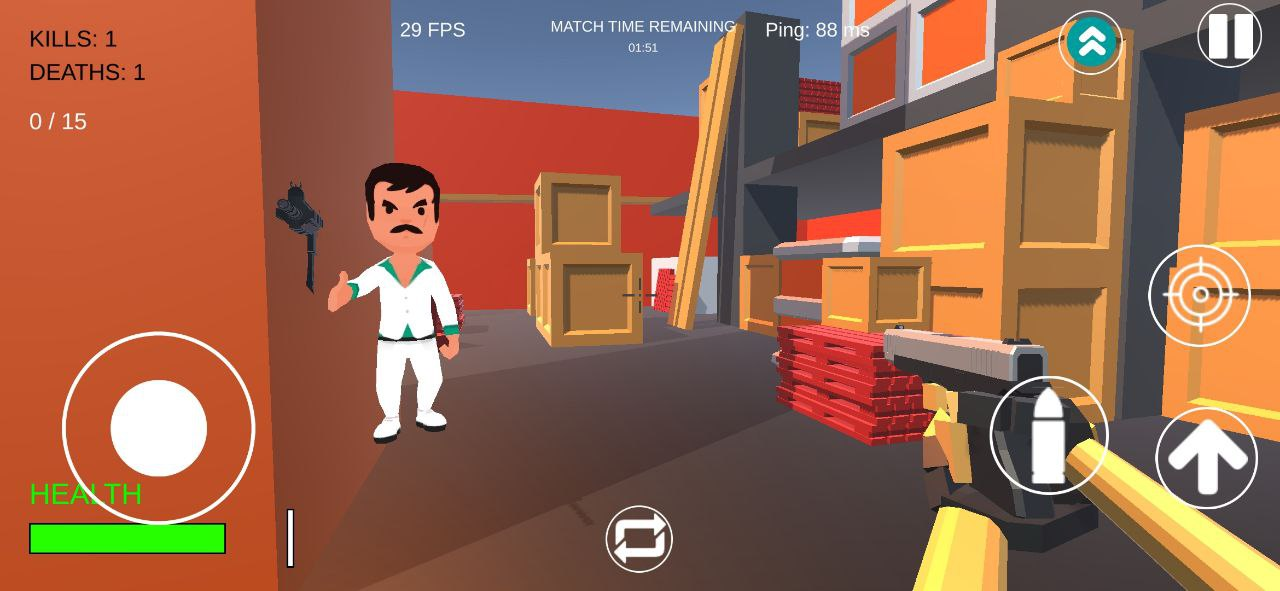
\includegraphics[width=8cm]{pergerakan.jpg}
        \caption{Tampilan Sinkronisasi Pergerakan}
        \label{fig:pergerakan}
    \end{figure}
    \newpage
    \begin{figure}[h]
        \centering
        \includegraphics[width=10cm]{leaderboard.jpg}
        \caption{Tampilan Sinkronisasi \textit{Kill} Dan \textit{Death}}
        \label{fig:leaderkill}
    \end{figure}
    \begin{figure}[h]
        \centering
        \includegraphics[width=10cm]{killed.jpg}
        \caption{Tampilan Sinkronisasi \textit{killed}}
        \label{fig:killed}
    \end{figure}
    \newpage
    \begin{figure}[h]
        \centering
        \includegraphics[width=10cm]{roundover.png}
        \caption{Tampilan Sinkronisasi \textit{Round Over}}
        \label{fig:roundover2}
    \end{figure}

    \subsection{Pengujian matchmaking}
    \noindent

    Pada uji coba ini menggunakan beberapa klien yang bersamaan memilih pencarian room / Pembuatan room. Aplikasi permainan harus terhubung ke internet terlebih dahulu agar dapat menggunakan fiture ini.
\begin{enumerate}
    \item Pengujian Mencari room \\
    Pada Pengujian ini player pertama mencari room yang dibuat oleh player kedua, dan pada pengujian pencarian room ini berhasil seperti gambar \ref{fig:pencarianroom}. 
    \begin{figure}[h]
        \centering
        \includegraphics[width=10cm]{pencarianroom.png}
        \caption{Tampilan Pencarian Room}
        \label{fig:pencarianroom}
    \end{figure}
    \item Pengujian Masuk Room \\
    Pada Pengujian memasuki room player berhasil menjumpai sesama player didalam room tersebut seperti gambar \ref{fig:didalamroom}.
    \begin{figure}[h]
        \centering
        \includegraphics[width=10cm]{5-player.png}
        \caption{Tampilan Didalam Room}
        \label{fig:didalamroom}
    \end{figure}
\end{enumerate}
\subsection{Pengujian QOS \textit{(Quality Of Service)}}
\noindent

Pengukuran QOS dilakukan untuk mengetahui performa jaringan dari photon unity networking.
\begin{enumerate}
    \item \textit{Packet Loss} \\
    Packet loss merupakan banyaknya paket yang gagal 
mencapai tempat tujuan paket tersebut dikirim. Ketika packet 
loss besar maka dapat diketahui bahwa jaringan sedang sibuk 
atau terjadi overload. Berdasarkan teori dan hasil pengamatan 
disaat melakukan pengukuran ,maka hasil yang didapatkan 
bisa dilihat pada \ref{tb:tabel-packetloss}.
\newpage
\begin{table}[h]
    \centering
    \caption{Hasil Pengukuran Packet loss}
    \label{tb:tabel-packetloss}
    \begin{tabular}{|c|c|c|c|c|} 
    \hline
    No & \begin{tabular}[c]{@{}c@{}}Hari\\Tanggal\end{tabular}        & Pengujian & Packet Loss & Tiphon        \\ 
    \hline
    1  & \begin{tabular}[c]{@{}c@{}}Rabu\\26 July\\2023\end{tabular}  & 1         & 0,1\%       & Sangat Bagus  \\ 
    \hline
    2  & \begin{tabular}[c]{@{}c@{}}Rabu\\26 July\\2023\end{tabular}  & 2         & 0\%         & Sangat Bagus  \\ 
    \hline
    3  & \begin{tabular}[c]{@{}c@{}}Rabu\\26 July \\2023\end{tabular} & 3         & 0,6\%       & Sangat Bagus  \\ 
    \hline
    4  & \begin{tabular}[c]{@{}c@{}}Rabu\\26~July\\2023\end{tabular}  & 4         & 0,2\%       & Sangat Bagus  \\ 
    \hline
    5  & \begin{tabular}[c]{@{}c@{}}Rabu\\26~July\\2023\end{tabular}  & 5         & 0\%         & Sangat Bagus  \\
    \hline
    \end{tabular}
    \end{table}

    Dari hasil pengukuran packet loss menurut standar TIPHON jika rata-rata packet loss 
0 maka masuk kedalam kategori “Sangat Bagus”.
\newpage
    \item \textit{Delay} \\
    Delay merupakan lamanya waktu yang dibutuhkan oleh 
    data atau informasi untuk sampai ke tempat tujuan data atau 
    informasi tersebut dikirim. Delay pada suatu jaringan akan 
    menentukan langkah apa yang akan kita ambil ketika kita 
    memanajemen suatu jaringan. Berdasarkan teori dan hasil 
    pengamatan disaat melakukan pengukuran ,maka hasil yang 
    didapatkan bisa dilihat pada \ref{tb:tabel-delay}
    
    \begin{table}[h]
        \centering
        \caption{Hasil Pengukuran Delay}
        \label{tb:tabel-delay}
        \begin{tabular}{|c|c|c|c|c|} 
        \hline
        No & \begin{tabular}[c]{@{}c@{}}Hari\\Tanggal\end{tabular}        & Pengujian & \begin{tabular}[c]{@{}c@{}}Delay\\Average\end{tabular} & Tiphon        \\ 
        \hline
        1  & \begin{tabular}[c]{@{}c@{}}Rabu\\26 July\\2023\end{tabular}  & 1         & 125                                                    & Sangat Bagus  \\ 
        \hline
        2  & \begin{tabular}[c]{@{}c@{}}Rabu\\26 July\\2023\end{tabular}  & 2         & 110                                                    & Sangat Bagus  \\ 
        \hline
        3  & \begin{tabular}[c]{@{}c@{}}Rabu\\26 July \\2023\end{tabular} & 3         & 125                                                    & Sangat Bagus  \\ 
        \hline
        4  & \begin{tabular}[c]{@{}c@{}}Rabu\\26~July\\2023\end{tabular}  & 4         & 90                                                     & Sangat Bagus  \\ 
        \hline
        5  & \begin{tabular}[c]{@{}c@{}}Rabu\\26~July\\2023\end{tabular}  & 5         & 130                                                    & Sangat Bagus  \\
        \hline
        \end{tabular}
        \end{table}
    
        Dari hasil pengukuran delay untuk masing-masing 
    pengguna adalah tertinggi terdapat di 1,3 dan 5 pengguna menurut standar TIPHON jika 
    rata-rata delay dibawah 150 ms maka masuk kedalam kategori 
    “Sangat Bagus”.
\end{enumerate}

\chapter{PENUTUP}
\section{Kesimpulan}
\noindent

Berdasarkan penelitian yang telah dilakuka oleh penulis, dapat diambil kesimpulan bahwa “Rancang Bangun Game Online FPS (Jak Meuprang) 3D Menggunakan Photon Unity Networking” berhasil dilakukan dengan kesimpulan sebagai berikut:
\begin{enumerate}
    \item Teknologi yang digunakan oleh penulis adalah Unity dengan menggunakan framework photon.
    \item Photon Unity Networking digunakan untuk memberikan permainan dapat dimainkan bersama sama dengan device yang berbeda-beda dan koneksi yang berbeda-beda.
    \item Hasil pengukuran QOS dapat disimpulkan jaringan yang disediakan oleh photon sangat bagus untuk versi gratisnya.
    \item Hasil pengujian sinkronisasi dapat disimpulkan bahwa saat player melakukan interaksi seperti bergerak,menembaki, dan waktu telah habis, maka interaksi tersebut dapat dilihat juga oleh player lainnya.
    \item Hasil pengujian dari hasil game yang telah dirancang yaitu game tersebut dapat dijalanka pada device menengah dengan fps rata rata 34FPS dan gui pada masing masing android sesuai dengan layar \textit{handphone} yang dimiliki.
\end{enumerate}

\section{Saran}
\noindent

Berdasarkan hasil dan kesimpulan yang telah disampaikan, terdapat beberapa kesimpulan inti yang dapat diambil dari penelitian ini. Selain itu, penulis juga ingin memberikan beberapa saran yang mungkin bermanfaat untuk pengembangan lebih lanjut. Adapun saran untuk pengembang game selanjutnya sebagai berikut:
\begin{enumerate}
    \item Menggunakan server Photon Unity Networking secara berbayar untuk mendapatkan pengalaman bermain secara online lebih luas dan dapat melebihi batas user yang telah ditentukan pada versi gratisnya.
    \item Menambahkan beberapa fiture senjata sebagai peningkatan. Senjata tersebut dapat ditambahkan dari berbagai senjata yang relavan dengan konteks modern.
    \item Menambahkan model karakter yang unik.
    \item Memperbaiki animationnya agar menjadi lebih baik.
\end{enumerate}

\bibliographystyle{apalike} % We choose the "plain" reference style
\bibliography{reference}
\addcontentsline{toc}{chapter}{DAFTAR PUSTAKA}

\end{document}
